\PassOptionsToPackage{unicode=true}{hyperref} % options for packages loaded elsewhere
\PassOptionsToPackage{hyphens}{url}
%
\documentclass[]{book}
\usepackage{lmodern}
\usepackage{amssymb,amsmath}
\usepackage{ifxetex,ifluatex}
\usepackage{fixltx2e} % provides \textsubscript
\ifnum 0\ifxetex 1\fi\ifluatex 1\fi=0 % if pdftex
  \usepackage[T1]{fontenc}
  \usepackage[utf8]{inputenc}
  \usepackage{textcomp} % provides euro and other symbols
\else % if luatex or xelatex
  \usepackage{unicode-math}
  \defaultfontfeatures{Ligatures=TeX,Scale=MatchLowercase}
\fi
% use upquote if available, for straight quotes in verbatim environments
\IfFileExists{upquote.sty}{\usepackage{upquote}}{}
% use microtype if available
\IfFileExists{microtype.sty}{%
\usepackage[]{microtype}
\UseMicrotypeSet[protrusion]{basicmath} % disable protrusion for tt fonts
}{}
\IfFileExists{parskip.sty}{%
\usepackage{parskip}
}{% else
\setlength{\parindent}{0pt}
\setlength{\parskip}{6pt plus 2pt minus 1pt}
}
\usepackage{hyperref}
\hypersetup{
            pdftitle={Elements of Nonparametric Statistics},
            pdfauthor={Nicholas Henderson},
            pdfborder={0 0 0},
            breaklinks=true}
\urlstyle{same}  % don't use monospace font for urls
\usepackage{color}
\usepackage{fancyvrb}
\newcommand{\VerbBar}{|}
\newcommand{\VERB}{\Verb[commandchars=\\\{\}]}
\DefineVerbatimEnvironment{Highlighting}{Verbatim}{commandchars=\\\{\}}
% Add ',fontsize=\small' for more characters per line
\usepackage{framed}
\definecolor{shadecolor}{RGB}{248,248,248}
\newenvironment{Shaded}{\begin{snugshade}}{\end{snugshade}}
\newcommand{\AlertTok}[1]{\textcolor[rgb]{0.94,0.16,0.16}{#1}}
\newcommand{\AnnotationTok}[1]{\textcolor[rgb]{0.56,0.35,0.01}{\textbf{\textit{#1}}}}
\newcommand{\AttributeTok}[1]{\textcolor[rgb]{0.77,0.63,0.00}{#1}}
\newcommand{\BaseNTok}[1]{\textcolor[rgb]{0.00,0.00,0.81}{#1}}
\newcommand{\BuiltInTok}[1]{#1}
\newcommand{\CharTok}[1]{\textcolor[rgb]{0.31,0.60,0.02}{#1}}
\newcommand{\CommentTok}[1]{\textcolor[rgb]{0.56,0.35,0.01}{\textit{#1}}}
\newcommand{\CommentVarTok}[1]{\textcolor[rgb]{0.56,0.35,0.01}{\textbf{\textit{#1}}}}
\newcommand{\ConstantTok}[1]{\textcolor[rgb]{0.00,0.00,0.00}{#1}}
\newcommand{\ControlFlowTok}[1]{\textcolor[rgb]{0.13,0.29,0.53}{\textbf{#1}}}
\newcommand{\DataTypeTok}[1]{\textcolor[rgb]{0.13,0.29,0.53}{#1}}
\newcommand{\DecValTok}[1]{\textcolor[rgb]{0.00,0.00,0.81}{#1}}
\newcommand{\DocumentationTok}[1]{\textcolor[rgb]{0.56,0.35,0.01}{\textbf{\textit{#1}}}}
\newcommand{\ErrorTok}[1]{\textcolor[rgb]{0.64,0.00,0.00}{\textbf{#1}}}
\newcommand{\ExtensionTok}[1]{#1}
\newcommand{\FloatTok}[1]{\textcolor[rgb]{0.00,0.00,0.81}{#1}}
\newcommand{\FunctionTok}[1]{\textcolor[rgb]{0.00,0.00,0.00}{#1}}
\newcommand{\ImportTok}[1]{#1}
\newcommand{\InformationTok}[1]{\textcolor[rgb]{0.56,0.35,0.01}{\textbf{\textit{#1}}}}
\newcommand{\KeywordTok}[1]{\textcolor[rgb]{0.13,0.29,0.53}{\textbf{#1}}}
\newcommand{\NormalTok}[1]{#1}
\newcommand{\OperatorTok}[1]{\textcolor[rgb]{0.81,0.36,0.00}{\textbf{#1}}}
\newcommand{\OtherTok}[1]{\textcolor[rgb]{0.56,0.35,0.01}{#1}}
\newcommand{\PreprocessorTok}[1]{\textcolor[rgb]{0.56,0.35,0.01}{\textit{#1}}}
\newcommand{\RegionMarkerTok}[1]{#1}
\newcommand{\SpecialCharTok}[1]{\textcolor[rgb]{0.00,0.00,0.00}{#1}}
\newcommand{\SpecialStringTok}[1]{\textcolor[rgb]{0.31,0.60,0.02}{#1}}
\newcommand{\StringTok}[1]{\textcolor[rgb]{0.31,0.60,0.02}{#1}}
\newcommand{\VariableTok}[1]{\textcolor[rgb]{0.00,0.00,0.00}{#1}}
\newcommand{\VerbatimStringTok}[1]{\textcolor[rgb]{0.31,0.60,0.02}{#1}}
\newcommand{\WarningTok}[1]{\textcolor[rgb]{0.56,0.35,0.01}{\textbf{\textit{#1}}}}
\usepackage{longtable,booktabs}
% Fix footnotes in tables (requires footnote package)
\IfFileExists{footnote.sty}{\usepackage{footnote}\makesavenoteenv{longtable}}{}
\usepackage{graphicx,grffile}
\makeatletter
\def\maxwidth{\ifdim\Gin@nat@width>\linewidth\linewidth\else\Gin@nat@width\fi}
\def\maxheight{\ifdim\Gin@nat@height>\textheight\textheight\else\Gin@nat@height\fi}
\makeatother
% Scale images if necessary, so that they will not overflow the page
% margins by default, and it is still possible to overwrite the defaults
% using explicit options in \includegraphics[width, height, ...]{}
\setkeys{Gin}{width=\maxwidth,height=\maxheight,keepaspectratio}
\setlength{\emergencystretch}{3em}  % prevent overfull lines
\providecommand{\tightlist}{%
  \setlength{\itemsep}{0pt}\setlength{\parskip}{0pt}}
\setcounter{secnumdepth}{5}
% Redefines (sub)paragraphs to behave more like sections
\ifx\paragraph\undefined\else
\let\oldparagraph\paragraph
\renewcommand{\paragraph}[1]{\oldparagraph{#1}\mbox{}}
\fi
\ifx\subparagraph\undefined\else
\let\oldsubparagraph\subparagraph
\renewcommand{\subparagraph}[1]{\oldsubparagraph{#1}\mbox{}}
\fi

% set default figure placement to htbp
\makeatletter
\def\fps@figure{htbp}
\makeatother

\usepackage[]{natbib}
\bibliographystyle{apalike}

\title{Elements of Nonparametric Statistics}
\author{Nicholas Henderson}
\date{2020-03-08}

\begin{document}
\maketitle

{
\setcounter{tocdepth}{1}
\tableofcontents
}
\hypertarget{preface}{%
\chapter*{Preface}\label{preface}}
\addcontentsline{toc}{chapter}{Preface}

This book will serve as the main source of course notes for Biostatistics 685/Statistics 560, Winter 2020.

\hypertarget{intro}{%
\chapter{Introduction}\label{intro}}

\begin{center}\rule{0.5\linewidth}{\linethickness}\end{center}

\begin{center}\rule{0.5\linewidth}{\linethickness}\end{center}

\hypertarget{sec:whatisnonpar}{%
\section{What is Nonparametric Statistics?}\label{sec:whatisnonpar}}

\textbf{What is Parametric Statistics?}

\begin{itemize}
\item
  Parametric models refer to probability distributions that can
  be fully described by a fixed number of parameters that do not change
  with the sample size.
\item
  Typical examples include

  \begin{itemize}
  \tightlist
  \item
    Gaussian
  \item
    Poisson
  \item
    Exponential
  \item
    Beta
  \end{itemize}
\item
  Could also refer to a regression setting where the mean function
  is described by a fixed number of parameters.
\end{itemize}

\textbf{What is Nonparametric Statistics?}

\begin{itemize}
\item
  It is difficult to give a concise, all-encompassing definition, but nonparametric
  statistics generally refers to statistical methods where there is not a clear parametric component.
\item
  A more practical definition is that nonparametric statistics refers to flexible statistical procedures where
  very few assumptions are made regarding the distribution of the data or the form
  of a regression model.
\item
  The uses of nonparametric methods in several common statistical contexts are described in Sections \ref{sec:example-nonpar-tests} - \ref{sec:example-nonpar-regress2}.
\end{itemize}

\hypertarget{sec:course-outline}{%
\section{Outline of Course}\label{sec:course-outline}}

This course is roughly divided into the following 5 categories.

\begin{enumerate}
\def\labelenumi{\arabic{enumi}.}
\tightlist
\item
  \textbf{Nonparametric Testing}
\end{enumerate}

\begin{itemize}
\tightlist
\item
  Rank-based Tests
\item
  Permutation Tests
\end{itemize}

\begin{enumerate}
\def\labelenumi{\arabic{enumi}.}
\tightlist
\item
  \textbf{Estimation of Basic Nonparametric Quantities}
\end{enumerate}

\begin{itemize}
\tightlist
\item
  The Empirical Distribution Function
\item
  Density Estimation
\end{itemize}

\begin{enumerate}
\def\labelenumi{\arabic{enumi}.}
\tightlist
\item
  \textbf{Nonparametric Confidence Intervals}
\end{enumerate}

\begin{itemize}
\tightlist
\item
  Bootstrap
\item
  Jacknife
\end{itemize}

\begin{enumerate}
\def\labelenumi{\arabic{enumi}.}
\tightlist
\item
  \textbf{Nonparametric Regression Part I (Smoothing Methods)}
\end{enumerate}

\begin{itemize}
\tightlist
\item
  Kernel Methods
\item
  Splines
\item
  Local Regression
\end{itemize}

\begin{enumerate}
\def\labelenumi{\arabic{enumi}.}
\tightlist
\item
  \textbf{Nonparametric Regression Part II (Machine Learning Methods)}
\end{enumerate}

\begin{itemize}
\tightlist
\item
  Decision Trees/CART
\item
  Ensemble Methods
\end{itemize}

\hypertarget{sec:example-nonpar-tests}{%
\section{Example 1: Nonparametric vs.~Parametric Two-Sample Testing}\label{sec:example-nonpar-tests}}

Suppose we have data from two groups. For example, outcomes from
two different treatments.

\begin{itemize}
\item
  \textbf{Group 1 outcomes}: \(X_{1}, \ldots, X_{n}\) an i.i.d (independent and identically distributed) sample from distribution function \(F_{X}\).
  This means that
  \begin{equation}
  F_{X}(t) = P( X_{i} \leq t) \quad \textrm{ for any } 1 \leq i \leq n  \nonumber
  \end{equation}
\item
  \textbf{Group 2 outcomes}: \(Y_{1}, \ldots, Y_{m}\) an i.i.d. sample from distribution function \(F_{Y}\).
  \begin{equation}
  F_{Y}(t) = P( Y_{i} \leq t) \quad \textrm{ for any } 1 \leq i \leq n  \nonumber
  \end{equation}
\item
  To test the impact of a new treatment, we usually want to test whether or not \(F_{X}\) differs from \(F_{Y}\) in some way.
  This can be stated in hypothesis testing language as
  \begin{eqnarray}
  H_{0}&:& F_{X} = F_{Y} \quad \textrm{( populations are the same)} \nonumber \\
  H_{A}&:& F_{X} \neq F_{Y} \quad \textrm{( populations are different)} \label{eq:nonpar-twosample-hypothesis}
                                                                        \end{eqnarray}
\end{itemize}

\textbf{Parametric Tests}

\begin{itemize}
\item
  Perhaps the most common parametric test for \eqref{eq:nonpar-twosample-hypothesis} is the \textbf{t-test}. The t-test assumes that
  \begin{equation}
  F_{X} = \textrm{Normal}(\mu_{x}, \sigma^{2}) \quad \textrm{ and } \quad F_{Y} = \textrm{Normal}(\mu_{y}, \sigma^{2})
  \end{equation}
\item
  Under this parametric assumption, the hypothesis test \eqref{eq:nonpar-twosample-hypothesis} reduces to
  \begin{equation}
  H_{0}: \mu_{x} = \mu_{y}  \quad \textrm{ vs. } \quad H_{A}: \mu_{x} \neq \mu_{y}
  \end{equation}
\item
  The standard t-statistic (with a pooled estimate of \(\sigma^{2}\)) is the following
  \begin{equation}
  T = \frac{\bar{X} - \bar{Y}}{ s_{p}\sqrt{\frac{1}{n} + \frac{1}{m}}  },
  \end{equation}
  where \(\bar{X} = \frac{1}{n}\sum_{i=1}^{n} X_{i}\) and \(\bar{Y} = \frac{1}{m}\sum_{i=1}^{m} Y_{i}\) are
  the group-specific sample means and \(s_{p}^{2}\) is the pooled estimate of \(\sigma^{2}\)
  \begin{equation}
  s_{p}^{2} = \frac{1}{m + n - 2}\Big\{ \sum_{i=1}^{n} (X_{i} - \bar{X})^{2} + \sum_{i=1}^{m} (Y_{i} - \bar{Y})^{2}   \Big\}
  \end{equation}
\end{itemize}

\begin{center}\rule{0.5\linewidth}{\linethickness}\end{center}

\begin{itemize}
\item
  The t-test is based on the \textbf{null distribution} of \(T\) - the distribution of \(T\) under the null hypothesis.
\item
  Under the assumption of normality, the null distribution of \(T\) is a t distribution with \(n + m - 2\) degrees of freedom.
\end{itemize}

\includegraphics{01-IntroductionLatex_files/figure-latex/unnamed-chunk-2-1.pdf}

\begin{itemize}
\item
  Notice that the null distribution of \(T\) depends on the parametric assumption that both \(F_{X} = \textrm{Normal}(\mu_{x}, \sigma^{2})\)
  and \(F_{Y} = \textrm{Normal}(\mu_{y}, \sigma^{2})\). Appealing to the Central Limit Theorem, one could
  argue that is a quite reasonable assumption.
\item
  In addition to using the assumption that \(F_{X} = \textrm{Normal}(\mu_{x}, \sigma^{2})\) and \(F_{Y} = \textrm{Normal}(\mu_{y}, \sigma^{2})\), we used this parametric assumption (at least implicitly) in the formulation of the hypothesis test itself because we assumed that any difference between \(F_{X}\) and \(F_{Y}\) would be fully described by difference in \(\mu_{x}\) and \(\mu_{y}\).
\item
  So, in a sense, you are using the assumption of normality twice in the construction of the two-sample t-test.
\end{itemize}

\begin{center}\rule{0.5\linewidth}{\linethickness}\end{center}

\textbf{Nonparametric Tests}

\begin{itemize}
\item
  Two-sample nonparametric tests are meant to be ``distribution-free''. This means the null distribution of the test statistic does not depend on any parametric
  assumptions about the two populations \(F_{X}\) and \(F_{Y}\).
\item
  Many such tests are based on \textbf{ranks}. The distribution of the ranks under the assumption that \(F_{X} = F_{Y}\) do
  not depend on the form of \(F_{X}\) (assuming \(F_{X}\) is continuous).
\item
  Also, the statements of hypotheses tests for nonparametric tests should not rely on any parametric assumptions about \(F_{X}\) and \(F_{Y}\).
\item
  For example, \(H_{A}: F_{X} \neq F_{Y}\) or \(H_{A}: F_{X} \geq F_{Y}\).
\end{itemize}

\begin{center}\rule{0.5\linewidth}{\linethickness}\end{center}

\begin{itemize}
\item
  Nonparametric tests usually tradeoff power for greater robustness.
\item
  In general, if the parametric assumptions are correct, a nonparametric test will have less power than its parametric counterpart.
\item
  If the parametric assumptions are not correct, parametric tests might have inappropriate type-I error control
  or lose power.
\end{itemize}

\hypertarget{sec:example-nonpar-estimation}{%
\section{Example 2: Nonparametric Estimation}\label{sec:example-nonpar-estimation}}

\begin{itemize}
\item
  Suppose we have \(n\) observations \((X_{1}, \ldots, X_{n})\) which are assumed to be i.i.d. (independent and identically distributed).
  The distribution function of \(X_{i}\) is \(F_{X}\).
\item
  Suppose we are interested in estimating the entire distribution function \(F_{X}\) rather than specific features
  of the distribution of \(X_{i}\) such as the mean or standard deviation.
\item
  In a \textbf{parametric} approach to estimating \(F_{X}\), we would assume the distribution of \(X_{i}\) belongs to some parametric family of distributions.
  For example,

  \begin{itemize}
  \tightlist
  \item
    \(X_{i} \sim \textrm{Normal}(\mu, \sigma^{2})\)
  \item
    \(X_{i} \sim \textrm{Exponential}(\lambda)\)
  \item
    \(X_{i} \sim \textrm{Beta}(\alpha, \beta)\)
  \end{itemize}
\end{itemize}

\begin{center}\rule{0.5\linewidth}{\linethickness}\end{center}

\begin{itemize}
\item
  If we assume that \(X_{i} \sim \textrm{Normal}( \mu, \sigma^{2} )\), we only need to estimate 2 parameters to
  fully describe the distribution of \(X_{i}\), and the number of parameters will not depend on the sample size.
\item
  In a nonparametric approach to characterizing the distribution of \(X_{i}\), we need to instead
  estimate the entire distribution function \(F_{X}\) or density function \(f_{X}\).
\item
  The distribution function \(F_{X}\) is usually estimated by the \textbf{empirical distribution function}
  \begin{equation}
  \hat{F}_{n}(t) = \frac{1}{n}\sum_{i=1}^{n} I( X_{i} \leq t),
  \end{equation}
  where \(I()\) denotes the indicator function. That is, \(I( X_{i} \leq t) = 1\) if \(X_{i} \leq t\),
  and \(I(X_{i} \leq t) = 0\) if \(X_{i} > t\).
\item
  The empirical distribution function is a discrete distribution function,
  and it can be thought of as an estimate having \(n\) "parameters.
\item
  The density function of \(X_{i}\) is often estimated by a kernel density estimator (KDE). This
  is defined as
  \begin{equation}
  \hat{f}_{n}(t) = \frac{1}{n h_{n}} \sum_{i=1}^{n} K\Big( \frac{t - X_{i}}{ h_{n} } \Big).
  \end{equation}
\item
  \(K()\) - the kernel function
\item
  \(h_{n}\) - the bandwidth
\item
  The KDE is a type of smoothing procedure.
\end{itemize}

\includegraphics{01-IntroductionLatex_files/figure-latex/unnamed-chunk-3-1.pdf} 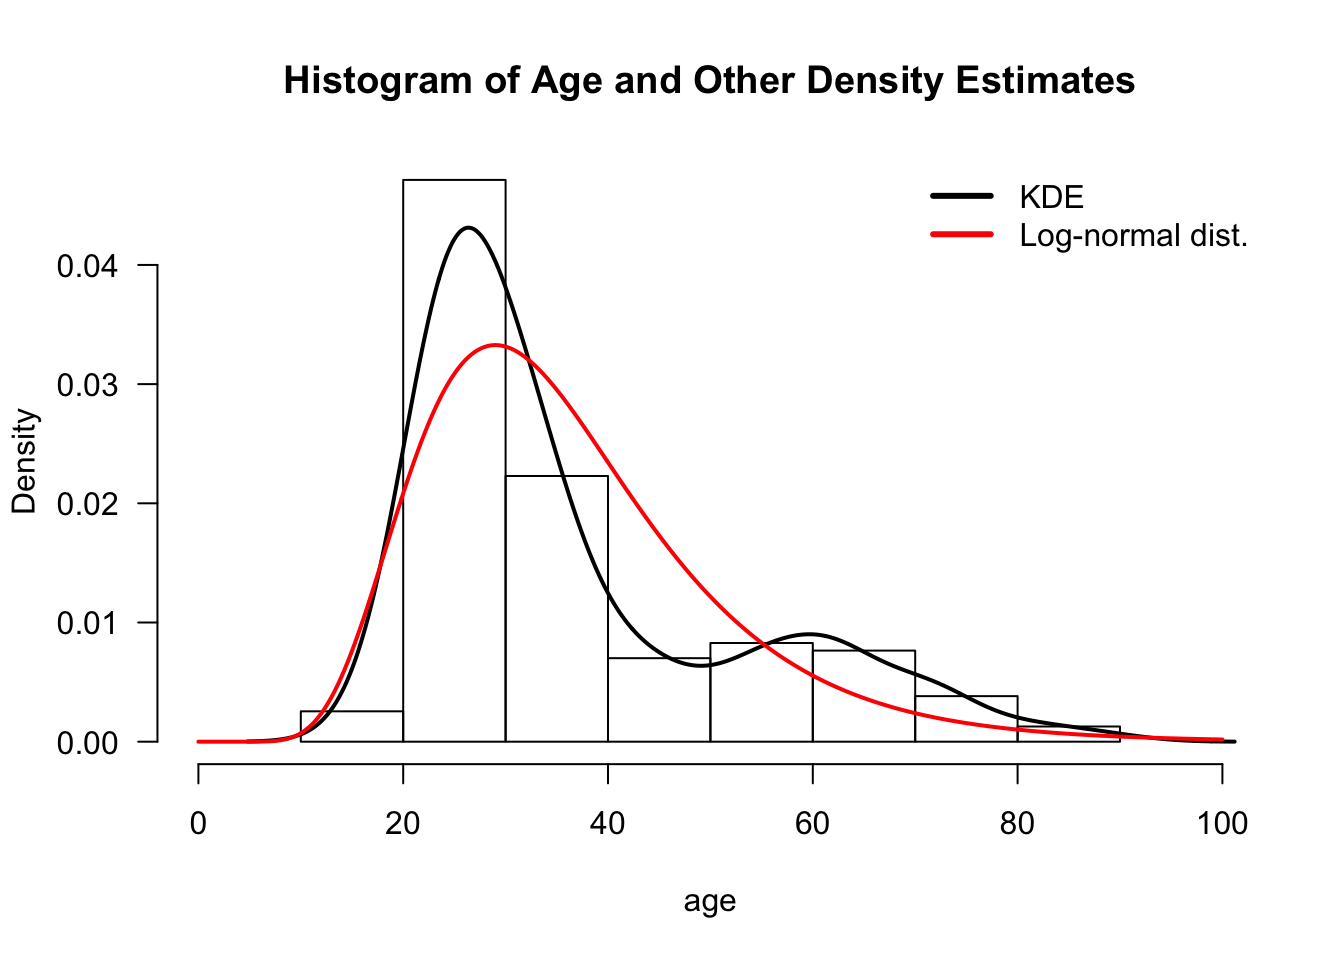
\includegraphics{01-IntroductionLatex_files/figure-latex/unnamed-chunk-3-2.pdf}

\hypertarget{sec:example-nonpar-confint}{%
\section{Example 3: Confidence Intervals}\label{sec:example-nonpar-confint}}

\begin{itemize}
\item
  Inference for a wide range of statistical procedures is based on the following argument
  \begin{equation}
  \hat{\theta}_{n} \textrm{ has an approximate Normal}\Big( \theta, \widehat{\textrm{Var}(\hat{\theta}_{n})} \Big) \textrm{ distribution }
  \label{eq:normal-approx}
  \end{equation}
\item
  Above, \(\hat{\theta}_{n}\) is an estimate of a parameter \(\theta\), and \(\widehat{\textrm{Var}(\hat{\theta}_{n})}\) is an estimate of the variance of \(\hat{\theta}_{n}\).
\item
  \(se_{n} = \sqrt{\widehat{\textrm{Var}(\hat{\theta}_{n})}}\) is usually referred to as the \textbf{standard error}.
\item
  \(95\%\) confidence intervals are reported using the following formula
  \begin{equation}
  [\hat{\theta}_{n} - 1.96 se_{n}, \hat{\theta}_{n} + 1.96 se_{n}  ]
  \end{equation}
\item
  Common examples of this include:

  \begin{enumerate}
  \def\labelenumi{\arabic{enumi}.}
  \tightlist
  \item
    \(\hat{\theta}_{n} = \bar{X}_{n}\).
  \end{enumerate}

  In this case, appeals to the Central Limit Theorem would justify approximation \eqref{eq:normal-approx}. The variance of \(\hat{\theta}_{n}\) would be \(\sigma^{2}\), and the standard error would typically be \(se_{n} = \hat{\sigma}/\sqrt{n}\).

  \begin{enumerate}
  \def\labelenumi{\arabic{enumi}.}
  \setcounter{enumi}{1}
  \tightlist
  \item
    \(\hat{\theta}_{n} = \textrm{Maximum Likelihood Estimate of } \theta\).
  \end{enumerate}

  In this case, asymptotics would justify the approximate distribution \(\hat{\theta}_{n} \sim \textrm{Normal}(\theta, \frac{1}{nI(\theta)} )\), where \(I(\theta)\) denotes the Fisher information. The standard error in this context is often \(se_{n} = \{ n I(\hat{\theta}_{n}) \}^{-1/2}\).
\end{itemize}

\begin{center}\rule{0.5\linewidth}{\linethickness}\end{center}

\begin{itemize}
\item
  Confidence intervals using \eqref{eq:normal-approx} rely on a parametric approximation to the
  sampling distribution of the statistic \(\hat{\theta}_{n}\).
\item
  Moreover, even if one wanted to use something like \eqref{eq:normal-approx}, working out
  standard error formulas can be a great challenge in more complicated situations.
\end{itemize}

\begin{center}\rule{0.5\linewidth}{\linethickness}\end{center}

\begin{itemize}
\item
  The \textbf{bootstrap} is a simulation-based approach for computing standard errors and
  confidence intervals.
\item
  The bootstrap does not rely on any particular parametric assumptions and
  can be applied in almost any context
  (though bootstrap confidence intervals can fail to work as desired in some situations).
\item
  Through resampling from the original dataset, the bootstrap uses many possible alternative datasets to
  assess the variability in \(\hat{\theta}_{n}\).
\end{itemize}

\begin{table}[ht]
\centering
\begin{tabular}{cccccc}
  \hline
 & OriginalDat & Dat1 & Dat2 & Dat3 & Dat4 \\ 
  \hline
Obs. 1 & 0.20 & 0.20 & 0.80 & 0.20 & 0.30 \\ 
  Obs. 2 & 0.50 & 0.20 & 0.80 & 0.20 & 0.70 \\ 
  Obs. 3 & 0.30 & 0.30 & 0.50 & 0.80 & 0.20 \\ 
  Obs. 4 & 0.80 & 0.30 & 0.70 & 0.50 & 0.50 \\ 
  Obs. 5 & 0.70 & 0.70 & 0.20 & 0.30 & 0.20 \\ 
  theta.hat & 0.50 & 0.34 & 0.60 & 0.40 & 0.38 \\ 
   \hline
\end{tabular}
\end{table}

\begin{center}\rule{0.5\linewidth}{\linethickness}\end{center}

\begin{itemize}
\item
  In the above example, we have 4 \textbf{boostrap replications} for the statistic \(\hat{\theta}\):
  \begin{eqnarray}
  \hat{\theta}^{(1)} &=& 0.34 \\ 
  \hat{\theta}^{(2)} &=& 0.60 \\
  \hat{\theta}^{(3)} &=& 0.40 \\ 
  \hat{\theta}^{(4)} &=& 0.38
  \end{eqnarray}
\item
  In the above example, the bootstrap standard error for \(\hat{\theta}_{n}\) would be
  the standard deviation of the bootstrap replications
  \begin{eqnarray}
  se_{boot} &=& \Big( \frac{1}{3} \sum_{b=1}^{4} \{ \hat{\theta}^{(b)} - \hat{\theta}^{(-)}  \}^{2} \Big)^{1/2} \nonumber \\
  &=& \Big( (0.34 - 0.43)^{2}/3 + (0.60 - 0.43)^{2}/3 + (0.40 - 0.43)^{2}/3 + (0.38 - 0.43)^{2}/3 \Big)^{1/2} \nonumber \\
  &=& 0.116
  \end{eqnarray}
  where \(\hat{\theta}^{(-)} = 0.43\) is the average of the bootstrap replications.
\item
  One would then report the confidence interval \([\hat{\theta} - 1.96 \times 0.116, \hat{\theta} + 1.96 \times 0.116]\).
  In practice, the number of bootstrap replications is typically much larger than \(4\).
\item
  It is often better to construct confidence intervals using the percentiles from the bootstrap distribution
  of \(\hat{\theta}\) rather than use a confidence interval of the form: \(\hat{\theta} \pm 1.96 \times se_{boot}\).
\end{itemize}

\begin{figure}
\centering
\includegraphics{01-IntroductionLatex_files/figure-latex/unnamed-chunk-4-1.pdf}
\caption{\label{fig:unnamed-chunk-4}Bootstrap distribution of the sample standard deviation for the age variable from the kidney fitness data. Dasjed vertical lines are placed at the 2.5 and 97.5 percentiles of the bootstrap distribution.}
\end{figure}

\hypertarget{sec:example-nonpar-regress1}{%
\section{Example 4: Nonparametric Regression with a Single Covariate}\label{sec:example-nonpar-regress1}}

\begin{itemize}
\item
  Regression is a common way of modeling the relationship between two different variables.
\item
  Suppose we have \(n\) pairs of observations \((y_{1}, x_{1}), \ldots, (y_{n}, x_{n})\) where
  \(y_{i}\) and \(x_{i}\) are suspected to have some association.
\item
  Linear regression would assume that these \(y_{i}\) and \(x_{i}\) are related by the following
  \begin{equation}
  y_{i} = \beta_{0} + \beta_{1}x_{i} + \varepsilon_{i} 
  \end{equation}
  with the assumption \(\varepsilon_{i} \sim \textrm{Normal}(0, \sigma^{2})\) often made.
\item
  In this model, there are only 3 parameters: \((\beta_{0}, \beta_{1}, \sigma^{2})\),
  and the number of parameters stays fixed for all \(n\).
\end{itemize}

\includegraphics{01-IntroductionLatex_files/figure-latex/unnamed-chunk-5-1.pdf}

\begin{center}\rule{0.5\linewidth}{\linethickness}\end{center}

\begin{itemize}
\item
  The nonparametric counterpart to linear regression is usually formulated in the following way
  \begin{equation}
  y_{i} = m( x_{i} ) + \varepsilon_{i}
  \end{equation}
\item
  Typically, one makes very few assumptions about the form of the mean function \(m\), and it is not assumed \(m\)
  can be described by a finite number of parameters.
\item
  There are a large number of nonparametric methods for estimating \(m\).
\item
  One popular method is the use of \textbf{smoothing splines}.
\item
  With smoothing splines, one considers mean functions of the form
  \begin{equation}
  m(x) = \sum_{j=1}^{n} \beta_{j}g_{j}(x) 
  \label{eq:smoothspline-model}
  \end{equation}
  where \(g_{1}, \ldots, g_{n}(x)\) are a collection of spline basis functions.
\end{itemize}

\begin{center}\rule{0.5\linewidth}{\linethickness}\end{center}

\begin{itemize}
\item
  Because of the large number of parameters in \eqref{eq:smoothspline-model}, one should
  estimate the basis function weights \(\beta_{j}\) through penalized regression
  \begin{equation}
  \textrm{minimize} \quad \sum_{i=1}^{n} \Big( y_{i} - \sum_{j=1}^{n} \beta_{j}g_{j}( x_{i} ) \Big)^{2} + \lambda \sum_{i=1}^{n}\sum_{j=1}^{n} \Omega_{ij}\beta_{i}\beta_{j}
  \label{eq:smoothspline-estimation}
  \end{equation}
  where \(\Omega_{ij} = \int g_{i}''(t)g_{j}''(t) dt\).
\item
  Using coefficient estimates \(\hat{\beta}_{1}, \ldots, \hat{\beta}_{n}\) found from solving \eqref{eq:smoothspline-model}, the nonparametric estimate of the mean function is defined as
  \begin{equation}
  \hat{m}(x) = \sum_{j=1}^{n} \hat{\beta}_{j}g_{j}(x) 
  \end{equation}
\item
  While the estimation in \eqref{eq:smoothspline-estimation} resembles parametric estimation for linear regression, notice
  that the number of parameters to be estimated will change with the sample size.
\item
  Allowing the number of basis functions to grow with \(n\) is important. For a sufficiently large number of basis functions, one should be able to approximate the
  true mean function \(m(x)\) arbitrarily closely.
\end{itemize}

\includegraphics{01-IntroductionLatex_files/figure-latex/unnamed-chunk-6-1.pdf}

\hypertarget{sec:example-nonpar-regress2}{%
\section{Example 5: Classification and Regression Trees (CART)}\label{sec:example-nonpar-regress2}}

\begin{itemize}
\item
  Suppose we now have observations \((y_{1}, \mathbf{x}_{1}), \ldots, (y_{n}, \mathbf{x}_{n})\) where
  \(y_{i}\) is a continuous response and \(\mathbf{x}_{i}\) is a p-dimensional vector of covariates.
\item
  Regression trees are a nonparametric approach for predicting \(y_{i}\) from \(\mathbf{x}_{i}\).
\item
  Here, the regression function is a \textbf{decision tree} rather than some fitted curve.
\item
  With a decision tree, a final prediction from a covariate vector \(\mathbf{x}_{i}\) is obtained by answering
  a sequence of ``yes or no'' questions.
\item
  When the responses \(y_{i}\) are binary, such trees are referred to as classification trees.
  Hence, the name: classification and regression trees (CART).
\end{itemize}

\includegraphics{01-IntroductionLatex_files/figure-latex/unnamed-chunk-7-1.pdf}

\includegraphics{01-IntroductionLatex_files/figure-latex/unnamed-chunk-8-1.pdf}

\begin{center}\rule{0.5\linewidth}{\linethickness}\end{center}

\begin{itemize}
\item
  Classification and regression trees are constructed through \textbf{recursive partitioning}.
\item
  Recursive partitioning is the process of deciding if and how to split a given
  node into two child nodes.
\item
  Tree splits are usually chosen to minimize the ``within-node'' sum of squares.
\item
  The size of the final is determined by a process of ``pruning'' the tree
  with cross-validation determining the best place to stop pruning.
\item
  Regression trees are an example of a more algorithmic approach to
  constructing predictions (as opposed to probability modeling in more
  traditional statistical methods) with a strong emphasis on predictive
  performance as measured through cross-validation.
\end{itemize}

\begin{center}\rule{0.5\linewidth}{\linethickness}\end{center}

\begin{itemize}
\item
  While single regression trees have the advantage of being directly interpretable,
  their prediction performance is often not that great.
\item
  However, using collections of trees can be very effective for prediction and
  has been used in many popular learning methods. Examples include: random forests,
  boosting, and Bayesian additive regression trees (BART).
\item
  Methods such as these can perform well on much larger datasets. We will discuss
  additional methods if time allows.
\end{itemize}

\hypertarget{getting-started}{%
\chapter{Working with R}\label{getting-started}}

You can download R by visiting \url{https://www.r-project.org/} and clicking on the \textbf{download R} link. Follow the instructions
to complete installation. THe most recent version is version 3.6.2.

It is not necessary to use this, but I find \textbf{RStudio} to be a very useful integrated development environment (IDE)
for computing with \textbf{R}. \textbf{RStudio} may be downloaded and installed by visiting \url{https://rstudio.com/}

\hypertarget{part-nonparametric-testing}{%
\part{Nonparametric Testing}\label{part-nonparametric-testing}}

\hypertarget{rank-tests}{%
\chapter{Rank and Sign Statistics}\label{rank-tests}}

\hypertarget{ranks}{%
\section{Ranks}\label{ranks}}

\hypertarget{definition}{%
\subsection{Definition}\label{definition}}

\begin{itemize}
\item
  Suppose we have \(n\) observations \(\mathbf{X} = (X_{1}, \ldots, X_{n})\). The \textbf{rank} of the \(i^{th}\) observation \(R_{i}\) is defined as
  \begin{equation}
  R_{i} = R_{i}(\mathbf{X}) = \sum_{j=1}^{n} I( X_{i} \geq X_{j}) 
  \label{eq:rankdef}
  \end{equation}
  where
  \begin{equation}
  I(X_{i} \geq X_{j}) 
  = \begin{cases}
  1 & \text{ if } X_{i} \geq X_{j} \\
  0 & \text{ if } X_{i} < X_{j}
  \end{cases}
  \end{equation}
\item
  The largest observation has a rank of \(n\).
\item
  The smallest observation has a rank of \(1\) (if there are no ties).
\item
  I'm using the notation \(R_{i}(\mathbf{X})\) to emphasize that the rank
  of the \(i^{th}\) observations depends on the entire vector of observations
  rather than only the value of \(X_{i}\).
\item
  You can compute ranks in \textbf{R} using the \textbf{rank} function:
\end{itemize}

\begin{Shaded}
\begin{Highlighting}[]
\NormalTok{x <-}\StringTok{ }\KeywordTok{c}\NormalTok{(}\DecValTok{3}\NormalTok{, }\DecValTok{7}\NormalTok{, }\DecValTok{1}\NormalTok{, }\DecValTok{12}\NormalTok{, }\DecValTok{6}\NormalTok{)  }\CommentTok{## 5 observations}
\KeywordTok{rank}\NormalTok{(x)}
\end{Highlighting}
\end{Shaded}

\begin{verbatim}
## [1] 2 4 1 5 3
\end{verbatim}

\hypertarget{handling-ties}{%
\subsection{Handling Ties}\label{handling-ties}}

\begin{itemize}
\item
  In the definition of ranks shown in \eqref{eq:rankdef}, tied observations
  receive their maximum possible rank.
\item
  For example, suppose that \((X_{1}, X_{2}, X_{3}, X_{4}) = (0, 1, 1, 2)\).
  In this case, one could argue whether both observations 2 and 3 should be ranked
  \(2^{nd}\) or \(3^{rd}\) while observations \(1\) and \(4\) should unambiguously receive
  ranks of \(1\) and \(4\) respectively.
\item
  Under definition \eqref{eq:rankdef}, both observations \(2\) and \(3\) receive a rank of \(3\).
\item
  In \textbf{R}, handling ties that is consistent with definition \eqref{eq:rankdef} is done using the \textbf{ties.method = ``max''} argument
\end{itemize}

\begin{Shaded}
\begin{Highlighting}[]
\NormalTok{x <-}\StringTok{ }\KeywordTok{c}\NormalTok{(}\DecValTok{0}\NormalTok{, }\DecValTok{1}\NormalTok{, }\DecValTok{1}\NormalTok{, }\DecValTok{2}\NormalTok{)  }
\KeywordTok{rank}\NormalTok{(x, }\DataTypeTok{ties.method=}\StringTok{"max"}\NormalTok{)}
\end{Highlighting}
\end{Shaded}

\begin{verbatim}
## [1] 1 3 3 4
\end{verbatim}

\begin{itemize}
\tightlist
\item
  The default in \textbf{R} is to replace the ranks of tied observations with their ``average'' rank
\end{itemize}

\begin{Shaded}
\begin{Highlighting}[]
\NormalTok{x <-}\StringTok{ }\KeywordTok{c}\NormalTok{(}\DecValTok{0}\NormalTok{, }\DecValTok{1}\NormalTok{, }\DecValTok{1}\NormalTok{, }\DecValTok{2}\NormalTok{)  }
\KeywordTok{rank}\NormalTok{(x)}
\end{Highlighting}
\end{Shaded}

\begin{verbatim}
## [1] 1.0 2.5 2.5 4.0
\end{verbatim}

\begin{Shaded}
\begin{Highlighting}[]
\NormalTok{y <-}\StringTok{ }\KeywordTok{c}\NormalTok{(}\DecValTok{2}\NormalTok{, }\DecValTok{9}\NormalTok{, }\DecValTok{7}\NormalTok{, }\DecValTok{7}\NormalTok{, }\DecValTok{3}\NormalTok{, }\DecValTok{2}\NormalTok{, }\DecValTok{1}\NormalTok{)}
\KeywordTok{rank}\NormalTok{(y, }\DataTypeTok{ties.method=}\StringTok{"max"}\NormalTok{)}
\end{Highlighting}
\end{Shaded}

\begin{verbatim}
## [1] 3 7 6 6 4 3 1
\end{verbatim}

\begin{Shaded}
\begin{Highlighting}[]
\KeywordTok{rank}\NormalTok{(y)}
\end{Highlighting}
\end{Shaded}

\begin{verbatim}
## [1] 2.5 7.0 5.5 5.5 4.0 2.5 1.0
\end{verbatim}

\begin{center}\rule{0.5\linewidth}{\linethickness}\end{center}

\begin{itemize}
\item
  When defining ranks using the ``average'' or ``midrank'' approach to handling ties, replaces
  tied ranks with the average of the two ``adjacent'' ranks.
\item
  For example, if we have a vector of ranks \((R_{1}, R_{2}, R_{3}, R_{4})\) where \(R_{2} = R_{3} =3\) and \(R_{1} = 4\) and \(R_{4} = 1\), then the vector of modified ranks using the ``average'' approach to handling ties
  would be
  \begin{equation}
  (R_{1}', R_{2}', R_{3}', R_{4}') = \Big( 4, \frac{4 + 1}{2}, \frac{4 + 1}{2}, 1 \Big)
  \end{equation}
\item
  The ``average'' approach is the most common way of handling ties when computing the
  Wilcoxon rank sum statistic.
\end{itemize}

\hypertarget{properties-of-ranks}{%
\subsection{Properties of Ranks}\label{properties-of-ranks}}

Suppose \((X_{1}, \ldots, X_{n})\) is random sample from a continuous distribution \(F\) (so that the probability
of ties is zero). Then, the following properties hold for the associated ranks \(R_{1}, \ldots, R_{n}\).

\begin{itemize}
\tightlist
\item
  Each \(R_{i}\) follows a discrete uniform distribution
  \begin{equation}
  P(R_{i} = j) = 1/n, \quad \text{for any } j = 1, \ldots,n.
  \end{equation}
\item
  The expectation of \(R_{i}\) is
  \begin{equation}
  E( R_{i} ) = \sum_{j=1}^{n} j P(R_{i} = j) = \frac{1}{n}\sum_{j=1}^{n} j = \frac{(n+1)}{2}
  \label{eq:rank-expectation}
  \end{equation}
\item
  The variance of \(R_{i}\) is
  \begin{equation}
  \text{Var}( R_{i} ) = E( R_{i}^{2} ) - E(R_{i})^{2}
  = \frac{1}{n}\sum_{j=1}^{n} j^{2}  - \Big( \frac{n+1}{2} \Big)^{2}
  = \frac{ n^{2} - 1}{12}
  \end{equation}
\item
  The random variables \(R_{1}, \ldots, R_{n}\) are \textbf{not} independent (why?). However,
  the vector \(\mathbf{R}_{n} = (R_{1}, \ldots, R_{n})\) is uniformly distributed
  on the set of \(n!\) permutations of \((1,2,\ldots,n)\).
\end{itemize}

\begin{center}\rule{0.5\linewidth}{\linethickness}\end{center}

\textbf{Exercise 3.1}: Suppose \(X_{1}, X_{2}, X_{3}\) are i.i.d. observations from a continuous
distribution function \(F_{X}\). Compute the covariance matrix of the vector
of ranks \(\big( R_{1}(\mathbf{X}), R_{2}(\mathbf{X}), R_{3}( \mathbf{X} ) \big)\).

\textbf{Exercise 3.2}: Again, suppose that \(X_{1}, X_{2}, X_{3}, X_{4}\) are i.i.d. observations from a continuous
distribution function \(F_{X}\). Let \(T= R_{1}( \mathbf{X} ) + R_{2}(\mathbf{X})\). Compute \(P( T = j )\)
for \(j = 3, 4, 5, 6, 7\).

\begin{center}\rule{0.5\linewidth}{\linethickness}\end{center}

\hypertarget{the-wilcoxon-rank-sum-wrs-test-a-two-sample-test}{%
\section{The Wilcoxon Rank Sum (WRS) Test: A Two-Sample Test}\label{the-wilcoxon-rank-sum-wrs-test-a-two-sample-test}}

\hypertarget{goal-of-the-test}{%
\subsection{Goal of the Test}\label{goal-of-the-test}}

\begin{itemize}
\item
  The Wilcoxon Rank Sum (WRS) test (sometimes referred to as the Wilcoxon-Mann-Whitney test) is a popular,
  rank-based two-sample test.
\item
  The WRS test is used to test whether or not observations from one group tend to be larger (or smaller) than observations
  from the other group.
\item
  Suppose we have observations from two groups: \(X_{1}, \ldots, X_{n} \sim F_{X}\) and \(Y_{1}, \ldots, Y_{m} \sim F_{Y}\).
\item
  Roughly speaking, the WRS tests the following hypothesis
  \begin{eqnarray}
  H_{0}: && F_{X} = F_{Y} \quad \textrm{ versus }  \\
  H_{A}: && \textrm{Observations from } F_{X} \textrm{ tend to be larger than observations from } F_{Y} \nonumber
  \label{eq:general-wilcoxon-hypothesis}
  \end{eqnarray}
\end{itemize}

\begin{center}\rule{0.5\linewidth}{\linethickness}\end{center}

\begin{itemize}
\item
  What is meant by ``tend to be larger'' in the alternative hypothesis?
\item
  Two common ways of stating the alternative hypothesis for the WRS include

  \begin{enumerate}
  \def\labelenumi{\arabic{enumi}.}
  \tightlist
  \item
    The stochastic dominance alternative
    \begin{eqnarray}
    H_{0}: & & F_{X} = F_{Y} \quad \textrm{ versus } \nonumber \\
    H_{A}: & & F_{X} \textrm{ is stochastically larger than } F_{Y} 
    \label{eq:stochasticlarger-formulation}
    \end{eqnarray}
  \item
    The ``shift'' alternative
    \begin{eqnarray}
    H_{0}: & & F_{X} = F_{Y} \quad \textrm{ versus } \nonumber \\
    H_{A}: & & F_{X}(t) = F_{Y}(t - \Delta), \Delta > 0.
    \label{eq:shift-formulation}
    \end{eqnarray}
  \end{enumerate}
\item
  A distribution function \(F_{X}\) is said to be stochastically larger than
  \(F_{Y}\) if \(F_{X}(t) \leq F_{Y}(t)\) for all \(t\) with \(F_{X}(t) < F_{Y}(t)\)
  for at least one value of \(t\).
\item
  Note that the ``shift alternative'' implies stochastic dominance.
\item
  Why do we need to specify an alternative?
\end{itemize}

\begin{center}\rule{0.5\linewidth}{\linethickness}\end{center}

\begin{itemize}
\item
  It is often stated that the WRS test is a test
  of equal medians.
\item
  This is true under the assumption that the
  relevant alternative is of the form \(F_{X}(t) = F_{Y}(t - \Delta)\).
\item
  However, one could have a scenario where the two groups have equal medians, but
  the WRS test has a very high probability of rejecting \(H_{0}\).
\item
  In addition, in many applications, it is difficult to justify
  that the ``shift alternative'' is a reasonable model.
\item
  An alternative is to view the WRS test as performing the following
  hypothesis test:
  \begin{eqnarray}
  H_{0}: && P(X_{i} > Y_{j}) + \tfrac{1}{2}P(X_{i} = Y_{j}) = 1/2 \quad \textrm{ versus } \\
  H_{A}: && P(X_{i} > Y_{j}) + \tfrac{1}{2}P(X_{i} = Y_{j}) > 1/2
  \label{eq:mw-formulation}
  \end{eqnarray}
  See \citet{divine2018} for more discussion around this formulation of the
  WRS test.
\item
  The hypothesis test \eqref{eq:mw-formulation} makes fewer assumptions
  about how \(F_{X}\) and \(F_{Y}\) are related and is, in many cases, more interpretable.
\item
  For example, in medical applications, it is often more natural to
  answer the question: what is the probability that the outcome
  under treatment 1 is better than the outcome under treatment 2.
\item
  The justification of hypothesis test \eqref{eq:mw-formulation} comes through
  the close connection between the WRS test statistic \(W\) and the Mann-Whitney statistic \(U_{MW}\).
  Specifically, \(W = U_{MW} + n(n+1)/2\). (Although, often \(U_{MW}\) is defined as
  \(U_{MW} = mn + n(n+1)/2 - W\)).
\item
  The Mann-Whitney statistic divided by \(mn\) is an estimate of the probability:
  \begin{equation}
  P(X_{i} > Y_{j}) + \tfrac{1}{2}P(X_{i} = Y_{j}) = 1/2.
  \end{equation}
\end{itemize}

\begin{center}\rule{0.5\linewidth}{\linethickness}\end{center}

\begin{itemize}
\item
  The reason for stating \(H_{0}\) in \eqref{eq:mw-formulation} as
  \begin{equation}
  H_{0}: P(X_{i} > Y_{j}) + \tfrac{1}{2}P(X_{i} = Y_{j}) = 1/2 \quad \textrm{ versus } \\
  \end{equation}
  is to cover the case of either a continuous or discrete distribution.
\item
  When both \(X_{i}\) and \(Y_{j}\) are samples from a continuous distribution
  we will have \(P(X_{i} = Y_{j}) = 0\), and we should then think of the null
  hypothesis as \(H_{0}: P(X_{i} > Y_{j})\).
\item
  For the case when both \(X_{i}\) and \(Y_{j}\) have a discrete distribution,
  consider an example where \(X_{i}\) and \(Y_{j}\) have the same discrete
  distribution with probabilities \(P(X_{i} = 0) = p_{0}, P(X_{i} = 1) = p_{1}\),
  and \(P(X_{i} = 2) = 1 - p_{0} - p_{2}\).
\item
  With this common discrete distribution on \(\{0, 1, 2\}\), we can see
  that \(P(X_{i} > Y_{j}) + \tfrac{1}{2}P(X_{i} = Y_{j}) = 1/2\) because
  \begin{eqnarray}
  P(X_{i} > Y_{j}) + \frac{1}{2}P(X_{i} = Y_{j}&)& = P(X_{i}=1, Y_{j}=0) + P(X_{i} = 2, Y_{j}=0) + P(X_{i}=2, Y_{j}=1)  \nonumber \\
  &+& \frac{1}{2}\Big[P(X_{i}=0, Y_{j}=0) + P(X_{i} = 1, Y_{j}=1) + P(X_{i}=2, Y_{j}=2) \Big] \nonumber \\
  &=& p_{1}p_{0} + (1 - p_{1} - p_{0})p_{0} + (1 - p_{1} - p_{0})p_{1}  \nonumber \\
  &+&  p_{0}^{2} + p_{1}^{2} + \frac{1}{2} - p_{0} - p_{1} + p_{0}p_{1} \nonumber \\
  &=& 1/2 \nonumber
  \end{eqnarray}
\end{itemize}

\hypertarget{definition-of-the-wrs-test-statistic}{%
\subsection{Definition of the WRS Test Statistic}\label{definition-of-the-wrs-test-statistic}}

\begin{itemize}
\item
  The WRS test statistic is based on computing the sum of ranks (ranks based on the pooled sample)
  in one group.
\item
  If observations from group 1 tend to be larger than those from group 2, the average rank from group 1 should exceed the
  average rank from group 2.
\item
  A sufficiently large value of the average rank from group 1 will allow us to reject \(H_{0}\)
  in favor of \(H_{A}\).
\end{itemize}

\begin{center}\rule{0.5\linewidth}{\linethickness}\end{center}

\begin{itemize}
\item
  We will define the pooled data vector \(\mathbf{Z}\) as
  \begin{equation}
  \mathbf{Z} = (X_{1}, \ldots, X_{n}, Y_{1}, \ldots, Y_{m})
  \end{equation}
  This is a vector with length \(n + m\).
\item
  The Wilcoxon rank-sum test statistic \(W\) for testing hypotheses of the form \eqref{eq:general-wilcoxon-hypothesis}
  is then defined as
  \begin{equation}
  W = \sum_{i=1}^{n} R_{i}( \mathbf{Z} )
  \label{eq:wrs-formula}
  \end{equation}
\item
  In other words, the WRS test statistic is the sum of the ranks for those observations coming
  from group 1 (i.e., the group with the \(X_{i}\) as observations).
\item
  If the group 1 observations tend to, in fact, be larger than the group 2 observations,
  then we should expect the sum of the ranks in this group to be larger than the sum of the
  ranks from group 2.
\end{itemize}

\begin{center}\rule{0.5\linewidth}{\linethickness}\end{center}

\begin{itemize}
\item
  Under \(H_{0}\), we can treat both \(X_{i}\) and \(Y_{i}\) as being observations coming from
  a common distribution function \(F\).
\item
  Hence, the expectation of \(R_{i}(\mathbf{Z})\) under the null hypothesis is
  \begin{equation}
  E_{H_{0}}\{ R_{i}(\mathbf{Z}) \} = \frac{n + m + 1}{2}
  \end{equation}
  and thus the expectation of \(W\) under \(H_{0}\)
  \begin{equation}
  E_{H_{0}}( W ) = \sum_{i=1}^{n} E_{H_{0}}\{ R_{i}( \mathbf{Z} ) \}
  = \frac{ n(n + m + 1)  }{ 2 }
  \end{equation}
\item
  It can be shown that the variance of \(W\) under the null hypothesis is
  \begin{equation}
  \textrm{Var}_{H_{0}}( W ) = \frac{mn(m + n + 1)}{12}
  \end{equation}
\end{itemize}

\hypertarget{computing-p-values-for-the-wrs-test}{%
\subsection{Computing p-values for the WRS Test}\label{computing-p-values-for-the-wrs-test}}

\textbf{Exact Distribution}

\begin{itemize}
\item
  The p-value is found by computing the probability
  \begin{equation}
  \textrm{p-value} = P_{H_{0}}( W \geq w_{obs})
  \end{equation}
  where \(w_{obs}\) is the observed WRS test statistic that
  we get from our data.
\item
  Computing p-values for the WRS test requires us to
  work with the \textbf{null distribution} of \(W\). That is,
  the distribution of \(W\) under the assumption that
  \(F_{X} = F_{Y}\).
\item
  The exact null distribution is found by using the fact
  that each possible ordering of the ranks has the same probability.
  That is,
  \begin{equation}
  P\{ R_{1}(\mathbf{Z}) = r_{1}, \ldots, R_{n+m}(\mathbf{Z}) =  r_{n+m} \} = \frac{1}{(n + m)!},
  \end{equation}
  where \((r_{1}, \ldots, r_{n+m})\) is any permutation of the set \(\{1, 2, \ldots, n + m\}\).
  Note that the null distribution only depends on \(n\) and \(m\).
\item
  Also, there are \({n + m \choose n}\) possible ways to assign distinct ranks to group 1.
\item
  Consider an example with \(n = m = 2\). In this case, there are \({4 \choose 2} = 6\) distinct
  ways to assign 2 ranks to group 1.
  What is the null distribution of the WRS test statistic? Try to verify that
  \begin{eqnarray}
  P_{H_{0}}( W = 7) &=& 1/6 \nonumber \\
  P_{H_{0}}( W = 6 ) &=& 1/6 \nonumber \\
  P_{H_{0}}(W = 5) &=& 1/3  \nonumber \\
  P_{H_{0}}( W = 4 ) &=& 1/6  \nonumber \\
  P_{H_{0}}(W = 3) &=& 1/6. \nonumber 
  \end{eqnarray}
\end{itemize}

\begin{center}\rule{0.5\linewidth}{\linethickness}\end{center}

\textbf{Large-Sample Approximate Distribution}

\begin{itemize}
\item
  Looking at \eqref{eq:wrs-formula}, we can see that the
  WRS test statistic is a sum of nearly independent random variables
  (at least nearly independent for large \(n\) and \(m\)).
\item
  Thus, we can expect that an appropriately centered and scaled
  version of \(W\) should be approximately Normally distributed (recall the Central Limit Theorem).
\item
  The standardized version \(\tilde{W}\) of the WRS is defined as
  \begin{equation}
  \tilde{W} = \frac{W - E_{H_{0}}(W)}{ \sqrt{\textrm{Var}_{H_{0}}(W) }  }
  = \frac{W - n(n+m+1)/2}{ \sqrt{ mn(n + m + 1)/12 }  }
  \end{equation}
\item
  Under \(H_{0}\), \(\tilde{W}\) converges in distribution to a Normal\((0,1)\) random variable.
\item
  A p-value using this large-sample approximation would then be computed in the following
  way
  \begin{eqnarray}
  \textrm{p-value} &=& P_{H_{0}}( W \geq w_{obs}) 
  = P\Bigg( \frac{W - n(n+m+1)/2}{ \sqrt{ mn(n + m + 1)/12 }  } \geq \frac{w_{obs} - n(n+m+1)/2}{ \sqrt{ mn(n + m + 1)/12 }  }\Bigg)
  \nonumber \\
  &=& P_{H_{0}}\Big( \tilde{W} \geq \frac{w_{obs} - n(n+m+1)/2}{ \sqrt{ mn(n + m + 1)/12 }  }\Big)
  = 1 - \Phi\Bigg( \frac{w_{obs} - n(n+m+1)/2}{ \sqrt{ mn(n + m + 1)/12 }  }  \Bigg), \nonumber
  \end{eqnarray}
  where \(\Phi(t)\) denotes the cumulative distribution function of a standard Normal random variable.
\item
  Often, in practice, a continuity correction is applied when using this large-sample approximation.
  For example, we would compute the probability \(P_{H_{0}}(W \geq w_{obs} - 0.5)\) with the Normal approximation
  rather than \(P_{H_{0}}(W \geq w_{obs})\) directly.
\end{itemize}

\begin{center}\rule{0.5\linewidth}{\linethickness}\end{center}

\begin{itemize}
\item
  Many statistical software packages (including \textbf{R}) will not compute p-values using the exact distribution in
  the presence of ties.
\item
  The \textbf{coin} package in \textbf{R} does allow you to perform a permutation test in the presence of ties.
\item
  A ``two-sided'' Wilcoxon rank sum test can also be performed. The two-sided
  hypothesis tests could either be stated as
  \begin{eqnarray}
  H_{0}: & & F_{X} = F_{Y} \quad \textrm{ versus } \nonumber \\
  H_{A}: & & F_{X} \textrm{ is stochastically larger or smaller than } F_{Y} 
  \end{eqnarray}
  or
  \begin{eqnarray}
  H_{0}: & & F_{X} = F_{Y} \quad \textrm{ versus } \nonumber \\
  H_{A}: & & F_{X}(t) = F_{Y}(t - \Delta), \Delta \neq 0.
  \end{eqnarray}
  or
  \begin{eqnarray}
  H_{0}: && P(X_{i} > Y_{i}) + \tfrac{1}{2}P(X_{i} = Y_{i}) = 1/2 \quad \textrm{ versus } \\
  H_{A}: && P(X_{i} > Y_{i}) + \tfrac{1}{2}P(X_{i} = Y_{i}) \neq 1/2
  \end{eqnarray}
\end{itemize}

\begin{center}\rule{0.5\linewidth}{\linethickness}\end{center}

\textbf{Exercise 3.3.} Using the exact distribution, what is the smallest
possible one-sided p-value associated with the WRS test
for a fixed value of \(n\) and \(m\) (assuming the probability of ties is zero)?

\begin{center}\rule{0.5\linewidth}{\linethickness}\end{center}

\hypertarget{computing-the-wrs-test-in-r}{%
\subsection{Computing the WRS test in R}\label{computing-the-wrs-test-in-r}}

\begin{itemize}
\tightlist
\item
  To illustrate performing the WRS test in \textbf{R}, we can use the \textbf{wine} dataset from the \textbf{rattle.data} package.
  This dataset is also available from the UCI Machine Learning Repository.
\end{itemize}

\begin{Shaded}
\begin{Highlighting}[]
\KeywordTok{library}\NormalTok{(rattle.data)}
\KeywordTok{head}\NormalTok{(wine)}
\end{Highlighting}
\end{Shaded}

\begin{verbatim}
##   Type Alcohol Malic  Ash Alcalinity Magnesium Phenols Flavanoids Nonflavanoids
## 1    1   14.23  1.71 2.43       15.6       127    2.80       3.06          0.28
## 2    1   13.20  1.78 2.14       11.2       100    2.65       2.76          0.26
## 3    1   13.16  2.36 2.67       18.6       101    2.80       3.24          0.30
## 4    1   14.37  1.95 2.50       16.8       113    3.85       3.49          0.24
## 5    1   13.24  2.59 2.87       21.0       118    2.80       2.69          0.39
## 6    1   14.20  1.76 2.45       15.2       112    3.27       3.39          0.34
##   Proanthocyanins Color  Hue Dilution Proline
## 1            2.29  5.64 1.04     3.92    1065
## 2            1.28  4.38 1.05     3.40    1050
## 3            2.81  5.68 1.03     3.17    1185
## 4            2.18  7.80 0.86     3.45    1480
## 5            1.82  4.32 1.04     2.93     735
## 6            1.97  6.75 1.05     2.85    1450
\end{verbatim}

\begin{itemize}
\tightlist
\item
  This dataset contains three types of wine. We will only consider the first two.
\end{itemize}

\begin{Shaded}
\begin{Highlighting}[]
\NormalTok{wine2 <-}\StringTok{ }\KeywordTok{subset}\NormalTok{(wine, Type}\OperatorTok{==}\DecValTok{1} \OperatorTok{|}\StringTok{ }\NormalTok{Type}\OperatorTok{==}\DecValTok{2}\NormalTok{)}
\NormalTok{wine2}\OperatorTok{$}\NormalTok{Type <-}\StringTok{ }\KeywordTok{factor}\NormalTok{(wine2}\OperatorTok{$}\NormalTok{Type)}
\end{Highlighting}
\end{Shaded}

\begin{itemize}
\item
  Let's consider the difference in the level of magnesium across the two types of wine.
  \includegraphics{03-rankstatLatex_files/figure-latex/unnamed-chunk-6-1.pdf} 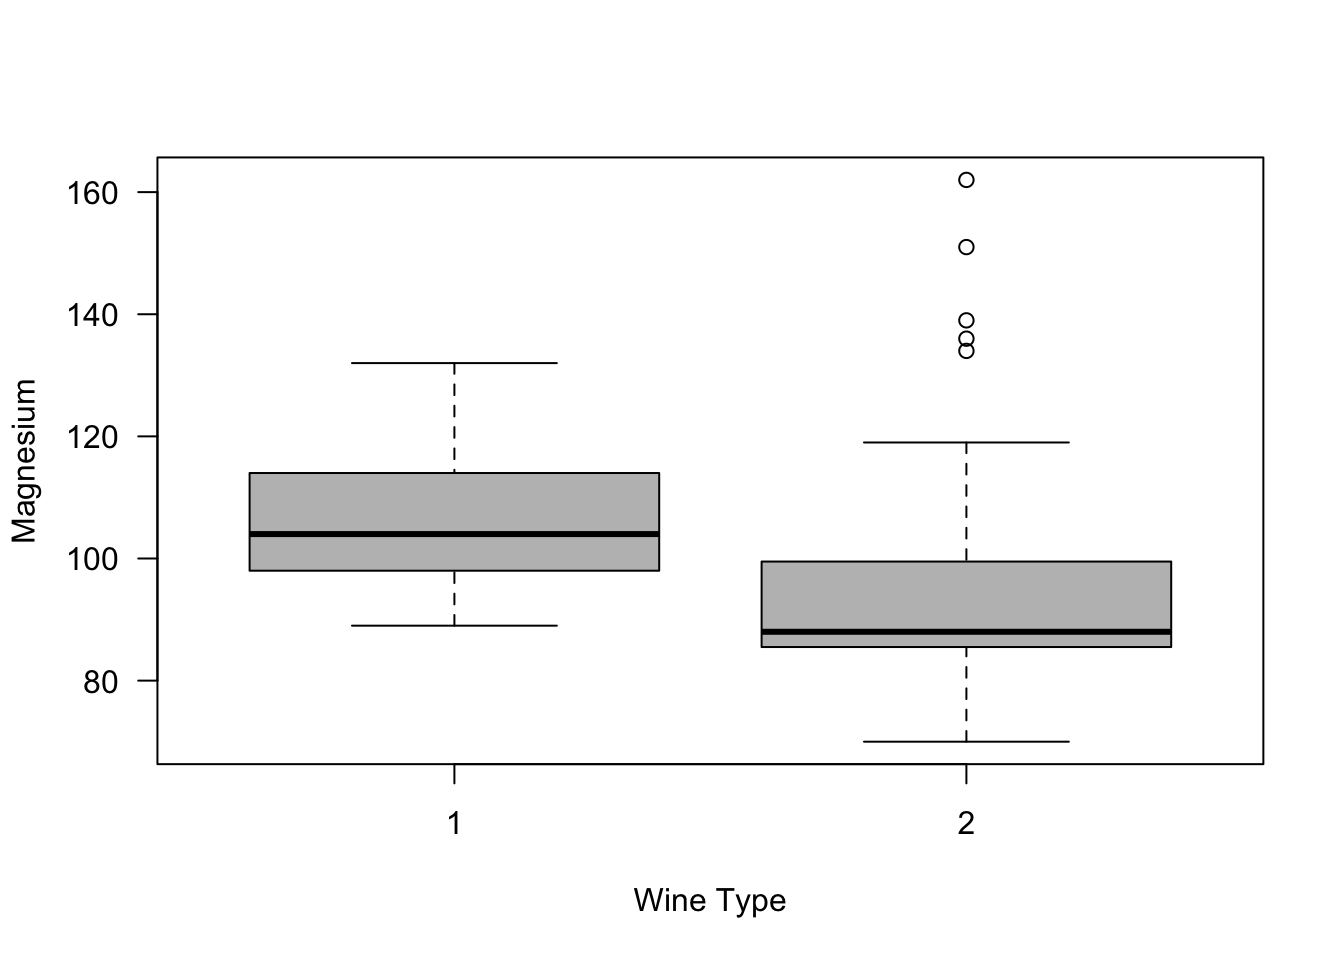
\includegraphics{03-rankstatLatex_files/figure-latex/unnamed-chunk-6-2.pdf}
\item
  Suppose we are interested in testing whether or not magnesium levels in
  Type 1 wine are generally larger than magnesium levels in Type 2 wine.
  This can be done with the following code
\end{itemize}

\begin{Shaded}
\begin{Highlighting}[]
\KeywordTok{wilcox.test}\NormalTok{(}\DataTypeTok{x=}\NormalTok{wine2}\OperatorTok{$}\NormalTok{Magnesium[wine2}\OperatorTok{$}\NormalTok{Type}\OperatorTok{==}\DecValTok{1}\NormalTok{], }\DataTypeTok{y=}\NormalTok{wine2}\OperatorTok{$}\NormalTok{Magnesium[wine2}\OperatorTok{$}\NormalTok{Type}\OperatorTok{==}\DecValTok{2}\NormalTok{], }
            \DataTypeTok{alternative=}\StringTok{"greater"}\NormalTok{)}
\end{Highlighting}
\end{Shaded}

\begin{verbatim}
## 
##  Wilcoxon rank sum test with continuity correction
## 
## data:  wine2$Magnesium[wine2$Type == 1] and wine2$Magnesium[wine2$Type == 2]
## W = 3381.5, p-value = 8.71e-10
## alternative hypothesis: true location shift is greater than 0
\end{verbatim}

You could also use the following code (just be careful about the ordering of the levels of \textbf{Type})

\begin{Shaded}
\begin{Highlighting}[]
\KeywordTok{wilcox.test}\NormalTok{(Magnesium }\OperatorTok{~}\StringTok{ }\NormalTok{Type, }\DataTypeTok{data=}\NormalTok{wine2, }\DataTypeTok{alternative=}\StringTok{"greater"}\NormalTok{)}
\end{Highlighting}
\end{Shaded}

\begin{verbatim}
## 
##  Wilcoxon rank sum test with continuity correction
## 
## data:  Magnesium by Type
## W = 3381.5, p-value = 8.71e-10
## alternative hypothesis: true location shift is greater than 0
\end{verbatim}

\begin{itemize}
\tightlist
\item
  What is the value of the WRS test statistic? We can code this directly
  with the following steps:
\end{itemize}

\begin{Shaded}
\begin{Highlighting}[]
\NormalTok{W <-}\StringTok{ }\KeywordTok{wilcox.test}\NormalTok{(}\DataTypeTok{x=}\NormalTok{wine2}\OperatorTok{$}\NormalTok{Magnesium[wine2}\OperatorTok{$}\NormalTok{Type}\OperatorTok{==}\DecValTok{1}\NormalTok{], }\DataTypeTok{y=}\NormalTok{wine2}\OperatorTok{$}\NormalTok{Magnesium[wine2}\OperatorTok{$}\NormalTok{Type}\OperatorTok{==}\DecValTok{2}\NormalTok{])}

\NormalTok{n <-}\StringTok{ }\KeywordTok{sum}\NormalTok{(wine2}\OperatorTok{$}\NormalTok{Type}\OperatorTok{==}\DecValTok{1}\NormalTok{)}
\NormalTok{m <-}\StringTok{ }\KeywordTok{sum}\NormalTok{(wine2}\OperatorTok{$}\NormalTok{Type}\OperatorTok{==}\DecValTok{2}\NormalTok{)}
\NormalTok{zz <-}\StringTok{ }\KeywordTok{rank}\NormalTok{(wine2}\OperatorTok{$}\NormalTok{Magnesium) }\CommentTok{## vector of pooled ranks}
\KeywordTok{sum}\NormalTok{(zz[wine2}\OperatorTok{$}\NormalTok{Type}\OperatorTok{==}\DecValTok{1}\NormalTok{])  }\CommentTok{## The WRS test statistic}
\end{Highlighting}
\end{Shaded}

\begin{verbatim}
## [1] 5151.5
\end{verbatim}

\begin{itemize}
\tightlist
\item
  The statistic returned by the \textbf{wilcox.test} function is actually equal to \(W - n(n+1)/2\) not \(W\)
\end{itemize}

\begin{Shaded}
\begin{Highlighting}[]
\KeywordTok{sum}\NormalTok{(zz[wine2}\OperatorTok{$}\NormalTok{Type}\OperatorTok{==}\DecValTok{1}\NormalTok{]) }\OperatorTok{-}\StringTok{ }\NormalTok{n}\OperatorTok{*}\NormalTok{(n }\OperatorTok{+}\StringTok{ }\DecValTok{1}\NormalTok{)}\OperatorTok{/}\DecValTok{2}
\end{Highlighting}
\end{Shaded}

\begin{verbatim}
## [1] 3381.5
\end{verbatim}

\begin{Shaded}
\begin{Highlighting}[]
\NormalTok{W}\OperatorTok{$}\NormalTok{statistic}
\end{Highlighting}
\end{Shaded}

\begin{verbatim}
##      W 
## 3381.5
\end{verbatim}

\begin{itemize}
\tightlist
\item
  \(\{ W - n(n+1)/2 \}\) is equal to the Mann-Whitney statistic. Thus, \textbf{W\$statistic/(mn)} is
  an estimate of the probability \(P(X_{i} > Y_{j}) + P(X_{i} = Y_{j})/2\).
\end{itemize}

\begin{Shaded}
\begin{Highlighting}[]
\NormalTok{W}\OperatorTok{$}\NormalTok{statistic}\OperatorTok{/}\NormalTok{(m}\OperatorTok{*}\NormalTok{n)}
\end{Highlighting}
\end{Shaded}

\begin{verbatim}
##         W 
## 0.8072332
\end{verbatim}

\begin{itemize}
\tightlist
\item
  Let's check how the Mann-Whitney statistic matches a simulation-based estimate of this probability
\end{itemize}

\begin{Shaded}
\begin{Highlighting}[]
\NormalTok{ind1 <-}\StringTok{ }\KeywordTok{which}\NormalTok{(wine2}\OperatorTok{$}\NormalTok{Type}\OperatorTok{==}\DecValTok{1}\NormalTok{)}
\NormalTok{ind2 <-}\StringTok{ }\KeywordTok{which}\NormalTok{(wine2}\OperatorTok{$}\NormalTok{Type}\OperatorTok{==}\DecValTok{2}\NormalTok{)}
\NormalTok{xgreater <-}\StringTok{ }\KeywordTok{rep}\NormalTok{(}\DecValTok{0}\NormalTok{, }\DecValTok{100}\NormalTok{)}
\ControlFlowTok{for}\NormalTok{(k }\ControlFlowTok{in} \DecValTok{1}\OperatorTok{:}\DecValTok{100}\NormalTok{) \{}
\NormalTok{    xi <-}\StringTok{ }\KeywordTok{sample}\NormalTok{(ind1, }\DataTypeTok{size=}\DecValTok{1}\NormalTok{)}
\NormalTok{    yi <-}\StringTok{ }\KeywordTok{sample}\NormalTok{(ind2, }\DataTypeTok{size=}\DecValTok{1}\NormalTok{)}
\NormalTok{    xgreater[k] <-}\StringTok{ }\KeywordTok{ifelse}\NormalTok{(wine2}\OperatorTok{$}\NormalTok{Magnesium[xi] }\OperatorTok{>}\StringTok{ }\NormalTok{wine2}\OperatorTok{$}\NormalTok{Magnesium[yi], }\DecValTok{1}\NormalTok{, }\DecValTok{0}\NormalTok{) }\OperatorTok{+}\StringTok{ }
\StringTok{                   }\KeywordTok{ifelse}\NormalTok{(wine2}\OperatorTok{$}\NormalTok{Magnesium[xi] }\OperatorTok{==}\StringTok{ }\NormalTok{wine2}\OperatorTok{$}\NormalTok{Magnesium[yi], }\DecValTok{1}\OperatorTok{/}\DecValTok{2}\NormalTok{, }\DecValTok{0}\NormalTok{)}
\NormalTok{\}}
\KeywordTok{mean}\NormalTok{(xgreater)  }\CommentTok{## estimate of this probability}
\end{Highlighting}
\end{Shaded}

\begin{verbatim}
## [1] 0.82
\end{verbatim}

\hypertarget{additional-notes-for-the-wrs-test}{%
\subsection{Additional Notes for the WRS test}\label{additional-notes-for-the-wrs-test}}

\hypertarget{comparing-ordinal-data}{%
\subsubsection{Comparing Ordinal Data}\label{comparing-ordinal-data}}

\begin{itemize}
\item
  The WRS test is often suggested when comparing categorical data which are \textbf{ordinal}.
\item
  For example, we might have 4 categories:

  \begin{itemize}
  \tightlist
  \item
    Poor
  \item
    Fair
  \item
    Good
  \item
    Excellent
  \end{itemize}
\item
  In this case, there is a natural ordering of the categories
  but any numerical values assigned to these categories would be arbitrary.
\item
  In such cases, we might be interested in testing whether or not outcomes tend to be
  better in one group than the other rather than simply comparing whether or not
  the distribution is different between the two groups.
\item
  A WRS test is useful here since we can still compute ranks without having to
  choose aribtrary numbers for each category.
\item
  Thinking of the ``probability greater than alternative \eqref{eq:mw-formulation}''
  or ``stochastically larger than alternative \eqref{eq:stochasticlarger-formulation}'' interpretation
  of the WRS test is probably more reasonable than the ``shift alternative \eqref{eq:shift-formulation}'' interpretation.
\item
  Note that there will probably be many ties when comparing ordinal data.
\end{itemize}

\begin{center}\rule{0.5\linewidth}{\linethickness}\end{center}

\begin{itemize}
\item
  The Hodges-Lehmann Estimator \(\hat{\Delta}\) is an estimator of \(\Delta\) in the location-shift model
  \begin{equation}
  F_{X}(t) = F_{Y}(t - \Delta) \nonumber
  \end{equation}
\item
  The Hodges-Lehmann is defined as the median difference among all possible (group 1, group 2) pairs.
  Specifically,
  \begin{equation}
  \hat{\Delta} = \textrm{median}\{ (X_{i} - Y_{j}); i=1,\ldots,n; j=1,\ldots,m \} \nonumber
  \end{equation}
\item
  We won't discuss the Hodges-Lehmann estimator in detail in this course, but in
  many statistical software packages, the
  Hodges-Lehmann is often reported when computing the WRS test.
\item
  In \textbf{R}, the Hodges-Lehmann estimator can be obtained by using the \textbf{conf.int=TRUE}
  argument in the \textbf{wilcox.test} function
\end{itemize}

\begin{Shaded}
\begin{Highlighting}[]
\NormalTok{WC <-}\StringTok{ }\KeywordTok{wilcox.test}\NormalTok{(}\DataTypeTok{x=}\NormalTok{wine2}\OperatorTok{$}\NormalTok{Magnesium[wine2}\OperatorTok{$}\NormalTok{Type}\OperatorTok{==}\DecValTok{1}\NormalTok{], }\DataTypeTok{y=}\NormalTok{wine2}\OperatorTok{$}\NormalTok{Magnesium[wine2}\OperatorTok{$}\NormalTok{Type}\OperatorTok{==}\DecValTok{2}\NormalTok{],}
                  \DataTypeTok{conf.int=}\OtherTok{TRUE}\NormalTok{)}
\NormalTok{WC}\OperatorTok{$}\NormalTok{estimate     }\CommentTok{## The Hodges-Lehmann estimate}
\end{Highlighting}
\end{Shaded}

\begin{verbatim}
## difference in location 
##               14.00005
\end{verbatim}

\hypertarget{one-sample-tests}{%
\section{One Sample Tests}\label{one-sample-tests}}

\hypertarget{sign-test}{%
\subsection{The Sign Test}\label{sign-test}}

\hypertarget{motivation-and-definition}{%
\subsubsection{Motivation and Definition}\label{motivation-and-definition}}

\begin{itemize}
\item
  The \textbf{sign test} can be thought of as a test of whether or not
  the median of a distribution is greater than zero (or greater than some other fixed value \(\theta_{0}\)).
\item
  Frequently, the sign test is explained in the following context:

  \begin{itemize}
  \tightlist
  \item
    Suppose we have observations \(D_{1}, \ldots, D_{n}\) which arise from the model
    \begin{equation}
    D_{i} = \theta + \varepsilon_{i},
    \label{eq:general-location}
    \end{equation}
    where \(\varepsilon_{i}\) are iid random variables each with distribution function \(F_{\epsilon}\)
    that is assumed to have a median of zero. Moreover, we will assume the density function
    \(f_{\varepsilon}(t)\) is symmetric around zero.
  \end{itemize}
\item
  The distribution function of \(D_{i}\) is then
  \begin{equation}
  F_{D}(t) = P(D_{i} \leq t) = P(\varepsilon_{i} \leq t - \theta) = F_{\epsilon}(t - \theta)
  \end{equation}
\item
  Likewise the density function \(f_{D}(t)\) of \(D_{i}\) is given by
  \begin{equation}
  f_{D}(t) = f_{\epsilon}(t - \theta)
  \end{equation}
\item
  In this context, \(\theta\) is usually referred to as a \textbf{location parameter}.
\item
  The goal here is to test \(H_{0}: \theta = \theta_{0}\) vs. \(H_{A}: \theta > \theta_{0}\). (Often, \(\theta_{0} = 0\)).
\end{itemize}

\begin{center}\rule{0.5\linewidth}{\linethickness}\end{center}

\begin{itemize}
\tightlist
\item
  This sort of test usually comes up in the context of \textbf{paired data}.
  Common examples include

  \begin{itemize}
  \tightlist
  \item
    patients compared ``pre and post treatment''
  \item
    students before and after the introduction of a new teaching method
  \item
    comparison of ``matched'' individuals who are similar (e.g., same age, sex, education, etc.)
  \item
    comparing consistency of measurements made on the same objects
  \end{itemize}
\end{itemize}

\begin{table}[ht]
\centering
\begin{tabular}{ccc}
  \hline
 & Baseline\_Measure & Post\_Treatment\_Measure \\ 
  \hline
Patient 1 & Y1 & X1 \\ 
  Patient 2 & Y2 & X2 \\ 
  Patient 3 & Y3 & X3 \\ 
  Patient 4 & Y4 & X4 \\ 
   \hline
\end{tabular}
\end{table}

\begin{itemize}
\item
  In such cases, we have observations \(X_{i}\) and \(Y_{i}\) for \(i = 1,\ldots n\) where
  it is not necessarily reasonable to think of \(X_{i}\) and \(Y_{i}\) as independent.
\item
  We can define \(D_{i} = X_{i} - Y_{i}\) as the difference in the \(i^{th}\) pair.
\item
  With this setup, a natural question is whether or not the differences \(D_{i}\) tend to be
  greater than zero or not.
\end{itemize}

\begin{center}\rule{0.5\linewidth}{\linethickness}\end{center}

\begin{itemize}
\item
  The \textbf{sign} statistic \(S_{n}\) is defined as
  \begin{equation}
  S_{n} = \sum_{i=1}^{n} I( D_{i} > 0)
  \label{eq:sign-statistic}
  \end{equation}
\item
  If the null hypothesis \(H_{0}: \theta = 0\) is true, then we should expect that roughly half
  of the observations will be positive.
\item
  This suggests that we will reject \(H_{0}\) if \(S_{n} \geq c\) where \(c\) is a
  number that is greater than \(n/2\).
\end{itemize}

\hypertarget{null-distribution-and-p-values}{%
\subsubsection{Null Distribution and p-values}\label{null-distribution-and-p-values}}

\begin{itemize}
\item
  Notice that the sign statistic defined in \eqref{eq:sign-statistic} is the sum of independent
  Bernoulli random variable.
\item
  That is, we can think of \(Z_{i} = I(D_{i} > 0)\) as a random variable with success probability
  \(p( \theta )\) where the formula for \(p( \theta )\) is
  \begin{equation}
  p(\theta) = P(Z_{i} = 1) = P(D_{i} > 0) = 1 - F_{D}(0) = 1 - F_{\epsilon}( -\theta )
  \end{equation}
\item
  This implies that \(S_{n}\) is a binomial random variable
  with \(n\) trials and success probability \(p(\theta)\).
  That is,
  \begin{equation}
  S_{n} \sim \textrm{Binomial}(n, p(\theta) )
  \label{eq:signstat-distribution}
  \end{equation}
\item
  Because \(p(0) = 1/2\), \(S_{n} \sim \textrm{Binomial}(n, 1/2 )\) under \(H_{0}\).
\item
  Notice that the ``null distribution'' of the sign statistic is ``distribution free''
  in the sense that the distribution does not depend on the distribution of \(D_{i}\).
\item
  The p-value for the sign test can be computed by
  \begin{equation}
  \textrm{p-value} = P_{H_{0}}(S_{n} \geq s_{obs}) = \sum_{j=s_{obs}}^{n} P_{H_{0}}(S_{n} = j)
  = \sum_{j=s_{obs}}^{n} {n \choose j} \frac{1}{2^{n}},
  \end{equation}
  where \(s_{obs}\) is the observed value of the sign statistic.
\end{itemize}

\begin{Shaded}
\begin{Highlighting}[]
\CommentTok{### How to compute the p-value for the sign test using R}
\NormalTok{xx <-}\StringTok{ }\KeywordTok{rnorm}\NormalTok{(}\DecValTok{100}\NormalTok{)}
\NormalTok{sign.stat <-}\StringTok{ }\KeywordTok{sum}\NormalTok{(xx }\OperatorTok{>}\StringTok{ }\DecValTok{0}\NormalTok{)}
\DecValTok{1} \OperatorTok{-}\StringTok{ }\KeywordTok{pbinom}\NormalTok{(sign.stat }\OperatorTok{-}\StringTok{ }\DecValTok{1}\NormalTok{, }\DataTypeTok{size=}\DecValTok{100}\NormalTok{, }\DataTypeTok{prob=}\DecValTok{1}\OperatorTok{/}\DecValTok{2}\NormalTok{) }\CommentTok{## p-value for sign test}
\end{Highlighting}
\end{Shaded}

\begin{verbatim}
## [1] 0.3821767
\end{verbatim}

\begin{itemize}
\item
  The reason that this is the right expression using \textbf{R} is that for any positive integer \(w\)
  \begin{equation}
  P_{H_{0}}(S_{n} \geq w) = 1 - P_{H_{0}}(S_{n} < w) = 1 - P_{H_{0}}(S_{n} \leq w - 1)
  \end{equation}
  and the \textbf{R} function \textbf{pbinom(t, n, prob)} computes \(P(X \leq t)\) where \(X\) is
  a binomial random variable with \(n\) trials and success probability \textbf{prob}.
\item
  You can also perform the one-sided sign test by using the \textbf{binom.test} function in \textbf{R}.
\end{itemize}

\begin{Shaded}
\begin{Highlighting}[]
\NormalTok{btest <-}\StringTok{ }\KeywordTok{binom.test}\NormalTok{(sign.stat, }\DataTypeTok{n=}\DecValTok{100}\NormalTok{, }\DataTypeTok{p=}\FloatTok{0.5}\NormalTok{, }\DataTypeTok{alternative=}\StringTok{"greater"}\NormalTok{) }
\NormalTok{btest}\OperatorTok{$}\NormalTok{p.value}
\end{Highlighting}
\end{Shaded}

\begin{verbatim}
## [1] 0.3821767
\end{verbatim}

\hypertarget{two-sided-sign-test}{%
\subsubsection{Two-sided Sign Test}\label{two-sided-sign-test}}

\begin{itemize}
\item
  Notice that the number of negative values of \(D_{i}\) can be expressed as
  \begin{equation}
  \sum_{i=1}^{n} I(D_{i} < 0) = n - S_{n}
  \end{equation}
  if there are no observations that equal zero exactly. Large value of \(n - S_{n}\)
  would be used in favor of another possible one-sided alternative \(H_{A}: \theta < 0\).
\item
  If we now want to test the two-sided alternative
  \begin{equation}
  H_{0}: \theta = 0 \quad \textrm{ vs. }  \quad H_{A}: \theta \neq 0 \nonumber
  \end{equation}
  you would need to compute the probability under the null hypothesis of observing
  a ``more extreme'' observation than the one that was actually observed.
\item
  Extreme is defined by thinking about the fact that we would have rejected \(H_{0}\)
  if either \(S_{n}\) or \(n - S_{n}\) were very large.
\item
  For example, if \(n = 12\), then the expected value of the sign statistic would be \(6\).
  If \(s_{obs} = 10\), then the collection of ``more extreme'' events then this would be
  \(\leq 2\) and \(\geq 10\).
\item
  The two-sided p-value is determined by looking at the tail probabilities on both sides
  \begin{equation}
  \textrm{p-value} = 
  \begin{cases}
  P_{H_{0}}(S_{n} \geq s_{obs}) + P_{H_{0}}(S_{n} \leq n - s_{obs}) & \textrm{ if } s_{obs} \geq n/2 \\
  P_{H_{0}}(S_{n} \leq s_{obs}) + P_{H_{0}}(S_{n} \geq n - s_{obs}) & \textrm{ if } s_{obs} < n/2
  \end{cases}
  \end{equation}
\item
  It actually works out that
  \begin{equation}
  \textrm{p-value} = 
  \begin{cases}
  2 P_{H_{0}}(S_{n} \geq s_{obs})   & \textrm{ if } s_{obs} \geq n/2 \\
  2 P_{H_{0}}(S_{n} \leq s_{obs})   & \textrm{ if } s_{obs} < n/2
  \end{cases}
  \end{equation}
\item
  Also, you can note that this p-value would be the same that you would get from performing the test
  \(H_{0}: p = 1/2\) vs. \(H_{A}: p \neq 1/2\) when it is assumed that \(S_{n} \sim \textrm{Binomial}(n, p)\).
\item
  Another note: It is often suggested that one should drop observations which are exactly zero
  when performing the sign test.
\end{itemize}

\hypertarget{the-wilcoxon-signed-rank-test}{%
\subsection{The Wilcoxon Signed Rank Test}\label{the-wilcoxon-signed-rank-test}}

\begin{itemize}
\item
  The Wilcoxon signed rank test can be applied
  under the same scenario that we used the sign test.
\item
  One criticism of the sign test is that it ignores the magnitude
  of the observations.
\item
  For example, the sign test statistic \(S\) treats observations
  \(D_{i} = 0.2\) and \(D_{i}=3\) the same.
\item
  The \textbf{Wilcoxon signed rank statistic} \(T_{n}\) weights the
  signs of \(D_{i}\) by the rank of its absolute value.
\item
  Specifically, the Wilcoxon signed rank statistic is defined as
  \begin{equation}
  T_{n} = \sum_{i=1}^{n} \textrm{sign}( D_{i}) R_{i}( |\mathbf{D}| )
  \end{equation}
  where the \(\textrm{sign}\) function is defined as
  \begin{equation}
  \textrm{sign}(x) = \begin{cases}
  1 & \textrm{if } x > 0 \\
  0 & \textrm{if } x = 0 \\
  -1 & \textrm{if } x < 0
  \end{cases}
  \end{equation}
\item
  Here, \(R_{i}( |\mathbf{D}| )\) is the rank of the \(i^{th}\) element from the vector
  \(|\mathbf{D}| = (|D_{1}|, |D_{2}|, \ldots, |D_{n}|)\).
\item
  Intuitively, the Wilcoxon signed rank statistic is measuring whether
  or not large values of \(|D_{i}|\) tend to be associated with positive
  vs.~negative values of \(D_{i}\).
\end{itemize}

\begin{center}\rule{0.5\linewidth}{\linethickness}\end{center}

Discuss some of these in class

\textbf{Exercise 3.4.} Suppose we had data \((-2, 1, -1/2, 3/2, 3)\). What would
be the value of the Wilcoxon signed rank statistic?

\textbf{Exercise 3.5.} Under the assumptions of model \eqref{eq:general-location}, what is
the density function of \(|D_{i}|\) and \(-|D_{i}|\)?

\textbf{Exercise 3.6.} Under the assumptions of model \eqref{eq:general-location} and
assuming that \(\theta = 0\), show that the expectation of the Wilcoxon signed-rank
statistic is \(0\).

\begin{center}\rule{0.5\linewidth}{\linethickness}\end{center}

\hypertarget{asymptotic-distribution}{%
\subsubsection{Asymptotic Distribution}\label{asymptotic-distribution}}

\begin{itemize}
\item
  As mentioned in the above exercise, the expectation of \(T_{n}\) under \(H_{0}\) is zero.
\item
  It can be shown that the variance under the null hypothesis is
  \begin{equation}
  \textrm{Var}_{H_{0}}( T_{n} ) = \frac{n(2n + 1)(n + 1)}{6} \nonumber
  \end{equation}
\item
  Similar, to the large-sample approximation we used for the WRS test, we have the following
  asymptotic result for the Wilcoxon signed-rank test
  \begin{equation}
  \frac{T_{n}}{\sqrt{\textrm{Var}_{H_{0}}(T_{n}) }} \longrightarrow \textrm{Normal}(0,1) \quad \textrm{as } n \longrightarrow \infty
  \end{equation}
\item
  Because the variance of \(T\) is dominated by the term \(n^{3}/3\) for very large \(n\), we could also say that under \(H_{0}\)
  that
  \begin{equation}
  \frac{T_{n}}{\sqrt{n^{3}/3} } \longrightarrow \textrm{Normal}(0,1) \quad \textrm{as } n \longrightarrow \infty
  \end{equation}
  In other words, we can say that \(T_{n}\) has an approximately \(\textrm{Normal}(0, n^{3}/3)\) for large \(n\).
\end{itemize}

\hypertarget{exact-distribution}{%
\subsubsection{Exact Distribution}\label{exact-distribution}}

\begin{itemize}
\tightlist
\item
  The exact distribution of the Wilcoxon signed rank statistic \(T_{n}\)
  is somewhat more complicated than the exact distribution of the WRS test statistic.
  Nevertheless, there exists functions in \textbf{R} for working with this exact distribution.
\end{itemize}

\hypertarget{using-r-to-perform-the-sign-and-wilcoxon-tests}{%
\subsection{Using R to Perform the Sign and Wilcoxon Tests}\label{using-r-to-perform-the-sign-and-wilcoxon-tests}}

\begin{itemize}
\item
  Let's first look at the \textbf{Meat} data from the \textbf{PairedData} \textbf{R} package.
\item
  This data set contains 20 observations with measures of fat percentage using different
  measuring techniques.
\end{itemize}

\begin{Shaded}
\begin{Highlighting}[]
\KeywordTok{library}\NormalTok{(PairedData, }\DataTypeTok{quietly=}\OtherTok{TRUE}\NormalTok{, }\DataTypeTok{warn.conflicts=}\OtherTok{FALSE}\NormalTok{) }\CommentTok{## loading PairedData package}
\KeywordTok{data}\NormalTok{(Meat)  }\CommentTok{## loading Meat data}
\KeywordTok{head}\NormalTok{(Meat)}
\end{Highlighting}
\end{Shaded}

\begin{verbatim}
##   AOAC Babcock     MeatType
## 1 22.0    22.3       Wiener
## 2 22.1    21.8       Wiener
## 3 22.1    22.4       Wiener
## 4 22.2    22.5       Wiener
## 5 24.6    24.9   ChoppedHam
## 6 25.3    25.6 ChooppedPork
\end{verbatim}

\begin{itemize}
\tightlist
\item
  Define the differences \(D_{i}\) as the \textbf{Babcock} measurements minus the \textbf{AOAC} measures.
  We will drop the single observation that equals zero.
\end{itemize}

\begin{Shaded}
\begin{Highlighting}[]
\NormalTok{DD <-}\StringTok{ }\NormalTok{Meat[,}\DecValTok{2}\NormalTok{] }\OperatorTok{-}\StringTok{ }\NormalTok{Meat[,}\DecValTok{1}\NormalTok{]}
\NormalTok{DD <-}\StringTok{ }\NormalTok{DD[DD}\OperatorTok{!=}\DecValTok{0}\NormalTok{]}
\KeywordTok{hist}\NormalTok{(DD, }\DataTypeTok{main=}\StringTok{"Meat Data"}\NormalTok{, }\DataTypeTok{xlab=}\StringTok{"Difference in Measured Fat Percentage"}\NormalTok{, }\DataTypeTok{las=}\DecValTok{1}\NormalTok{)}
\end{Highlighting}
\end{Shaded}

\includegraphics{03-rankstatLatex_files/figure-latex/unnamed-chunk-17-1.pdf}

\begin{Shaded}
\begin{Highlighting}[]
\KeywordTok{summary}\NormalTok{(DD)}
\end{Highlighting}
\end{Shaded}

\begin{verbatim}
##     Min.  1st Qu.   Median     Mean  3rd Qu.     Max. 
## -1.60000 -0.25000  0.30000  0.04211  0.40000  1.10000
\end{verbatim}

\textbf{The Sign Test in R}

\begin{itemize}
\tightlist
\item
  Let's first test the hypothesis \(H_{0}: \theta = 0\) vs. \(H_{A}: \theta \neq 0\) using
  the two-sided sign test. This can be done using the \textbf{binom.test} function
\end{itemize}

\begin{Shaded}
\begin{Highlighting}[]
\KeywordTok{binom.test}\NormalTok{(}\KeywordTok{sum}\NormalTok{(DD }\OperatorTok{>}\StringTok{ }\DecValTok{0}\NormalTok{), }\DataTypeTok{n =} \KeywordTok{length}\NormalTok{(DD), }\DataTypeTok{p=}\FloatTok{0.5}\NormalTok{)}\OperatorTok{$}\NormalTok{p.value}
\end{Highlighting}
\end{Shaded}

\begin{verbatim}
## [1] 0.6476059
\end{verbatim}

\textbf{Wilcoxon Signed Rank Test in R}

\begin{itemize}
\tightlist
\item
  You can actually use the function \textbf{wilcox.test} to perform the Wilcoxon signed rank test in addition
  to the Wilcoxon rank sum test. To perform the Wilcoxon signed rank test in \textbf{R}, you just
  need to enter data for the \textbf{x} argument and leave the \textbf{y} argument empty.
\end{itemize}

\begin{Shaded}
\begin{Highlighting}[]
\KeywordTok{wilcox.test}\NormalTok{(}\DataTypeTok{x=}\NormalTok{DD)}
\end{Highlighting}
\end{Shaded}

\begin{verbatim}
## Warning in wilcox.test.default(x = DD): cannot compute exact p-value with ties
\end{verbatim}

\begin{verbatim}
## 
##  Wilcoxon signed rank test with continuity correction
## 
## data:  DD
## V = 118.5, p-value = 0.3534
## alternative hypothesis: true location is not equal to 0
\end{verbatim}

\begin{itemize}
\item
  You will note that the p-value for the Wilcoxon signed rank test is lower than that
  of the sign test. In general, the Wilcoxon signed rank test is somewhat more ``sensitive''
  than the sign test meaning that it will have a greater tendency
  to reject \(H_{0}\) for small deviations from \(H_{0}\).
\item
  We can explore this sensitivity comparison with a small simulation study. We
  will consider a scenario where \(D_{i} = 0.4 + \varepsilon_{i}\) with \(\varepsilon_{i}\)
  having a t distribution with \(3\) degrees of freedom.
\end{itemize}

\begin{Shaded}
\begin{Highlighting}[]
\KeywordTok{set.seed}\NormalTok{(}\DecValTok{1327}\NormalTok{)}
\NormalTok{n.reps <-}\StringTok{ }\DecValTok{500}  \CommentTok{## number of simulation replications}
\NormalTok{samp.size <-}\StringTok{ }\DecValTok{50}  \CommentTok{## the sample size}
\NormalTok{wilcox.reject <-}\StringTok{ }\KeywordTok{rep}\NormalTok{(}\DecValTok{0}\NormalTok{, n.reps)}
\NormalTok{sign.reject <-}\StringTok{ }\KeywordTok{rep}\NormalTok{(}\DecValTok{0}\NormalTok{, n.reps)}
\ControlFlowTok{for}\NormalTok{(k }\ControlFlowTok{in} \DecValTok{1}\OperatorTok{:}\NormalTok{n.reps) \{}
\NormalTok{    dsim <-}\StringTok{ }\FloatTok{.4} \OperatorTok{+}\StringTok{ }\KeywordTok{rt}\NormalTok{(samp.size, }\DataTypeTok{df=}\DecValTok{3}\NormalTok{)}
\NormalTok{    wilcox.reject[k] <-}\StringTok{ }\KeywordTok{ifelse}\NormalTok{(}\KeywordTok{wilcox.test}\NormalTok{(}\DataTypeTok{x=}\NormalTok{dsim)}\OperatorTok{$}\NormalTok{p.value }\OperatorTok{<}\StringTok{ }\FloatTok{0.05}\NormalTok{, }\DecValTok{1}\NormalTok{, }\DecValTok{0}\NormalTok{)}
\NormalTok{    sign.reject[k] <-}\StringTok{ }\KeywordTok{ifelse}\NormalTok{(}\KeywordTok{binom.test}\NormalTok{(}\KeywordTok{sum}\NormalTok{(dsim }\OperatorTok{>}\StringTok{ }\DecValTok{0}\NormalTok{), }
                                       \DataTypeTok{n=}\NormalTok{samp.size, }\DataTypeTok{p=}\FloatTok{0.5}\NormalTok{)}\OperatorTok{$}\NormalTok{p.value }\OperatorTok{<}\StringTok{ }\FloatTok{0.05}\NormalTok{, }\DecValTok{1}\NormalTok{, }\DecValTok{0}\NormalTok{)}
\NormalTok{\}}
\KeywordTok{mean}\NormalTok{(wilcox.reject)  }\CommentTok{## proportion of times Wilcoxon signed rank rejected H0}
\end{Highlighting}
\end{Shaded}

\begin{verbatim}
## [1] 0.614
\end{verbatim}

\begin{Shaded}
\begin{Highlighting}[]
\KeywordTok{mean}\NormalTok{(sign.reject)  }\CommentTok{## proportion of times Wilcoxon signed rank rejected H0}
\end{Highlighting}
\end{Shaded}

\begin{verbatim}
## [1] 0.488
\end{verbatim}

\hypertarget{power-and-comparisons-with-parametric-tests}{%
\section{Power and Comparisons with Parametric Tests}\label{power-and-comparisons-with-parametric-tests}}

\hypertarget{the-power-function-of-a-test}{%
\subsection{The Power Function of a Test}\label{the-power-function-of-a-test}}

\begin{itemize}
\item
  The \textbf{power} of a test is the probability
  that a test rejects the null hypothesis when the
  alternative hypothesis is true.
\item
  The alternative hypothesis \(H_{A}\) is usually characterized
  by a large range of values of the parameter of interest.
  For example, \(H_{A}: \theta > 0\) or \(H_{A}: \theta \neq 0\).
\item
  For this reason, it is better to think of power
  as a function that varies across the range
  of the alternative hypothesis.
\item
  To be more precise, we will define the power
  function as a function of some parameter \(\theta\)
  where the null hypothesis corresponds to \(\theta = \theta_{0}\)
  and the alternative hypothesis represents a range
  of alternative values of \(\theta\).
\item
  The power function \(\gamma_{n}(\cdot)\) of a testing procedure is defined as
  \begin{equation}
  \gamma_{n}(\delta) = P_{\theta=\delta}\{  \textrm{reject } H_{0} \} \qquad \textrm{ for } \delta \in H_{A}. \nonumber
  \end{equation}
\item
  The notation \(P_{\theta=\delta}\{ \textrm{reject } H_{0} \}\) means that we are computing this
  probability under the assumption that the parameter of interest \(\theta\) equals \(\delta\).
\end{itemize}

\begin{center}\rule{0.5\linewidth}{\linethickness}\end{center}

\textbf{The Approximate Power Function of the Sign Test}

\begin{itemize}
\item
  Let us consider the sign test for testing \(H_{0}: \theta = 0\) vs. \(\theta > 0\).
\item
  The sign test is based on the value of the sign statistic \(S_{n}\).
\item
  Recalling \eqref{eq:signstat-distribution}, we know that \(S_{n} \sim \textrm{Binomial}(n, p(\theta))\).
  Hence,
  \begin{equation}
  \sqrt{n}(\tfrac{S_{n}}{n} - p(\theta)) \longrightarrow \textrm{Normal}\Big( 0, p(\theta)(1 - p(\theta)) \Big) \quad \textrm{as } n \longrightarrow \infty
  \label{eq:approx-signstat}
  \end{equation}
\item
  The sign test will reject \(H_{0}\) when \(S_{n} \geq c_{\alpha,n}\) where the constant \(c_{\alpha,n}\) is chosen
  so that \(P_{H_{0}}( S_{n} \geq c_{\alpha,n} ) = \alpha\). Using the large-sample approximation \eqref{eq:approx-signstat}, you can
  show that
  \begin{equation}
  c_{\alpha, n} = \frac{n + \sqrt{n}z_{1-\alpha}}{2}, 
  \label{eq:critical-value-signstat}
  \end{equation}
  where \(z_{1-\alpha}\) denotes the upper \(1 - \alpha\) quantile of the standard normal distribution. In other words,
  \(\Phi( z_{1-\alpha}) = 1-\alpha\).
\item
  Also, when using large-sample approximation \eqref{eq:approx-signstat}, the power of this test to detect a value of \(\theta = \delta\) is given by
  \begin{eqnarray}
  \gamma_{n}(\delta) &=& P_{\theta=\delta}\{ S_{n} \geq c_{\alpha,n} \} 
  = P_{\theta=\delta}\Bigg\{ \frac{\sqrt{n}(S_{n}/n - p(\delta))}{\sqrt{ p(\delta)(1 - p(\delta)) } } \geq 
  \frac{ \sqrt{n}(c_{\alpha, n}/n - p(\delta)) }{ \sqrt{p(\delta)(1 - p(\delta))}  } \Bigg\}  \nonumber \\
  &=& 1 - \Phi\Bigg( \frac{ \sqrt{n}(c_{\alpha,n}/n - p(\delta)) }{ \sqrt{p(\delta)(1 - p(\delta))}  } \Bigg) \nonumber \\
  &=& 1 - \Phi\Bigg( \frac{ z_{1-\alpha} }{ 2\sqrt{p(\delta)(1 - p(\delta))}  } - \frac{ \sqrt{n}(p(\delta) - 1/2) }{ \sqrt{p(\delta)(1 - p(\delta))}  }\Bigg)
  \label{eq:powerfn-signstat}
  \end{eqnarray}
\item
  Notice that the power of the test depends more directly on the term \(p(\delta) = P_{\theta = \delta}(D_{i} > 0)\).
  Recall from Section \ref{sign-test} that
  \(p(\delta) = 1 - F_{\epsilon}(-\delta)\), where \(F_{\epsilon}\) is the distribution function
  of \(\varepsilon_{i}\) in the model \(D_{i} = \theta + \varepsilon_{i}\).
\item
  So, in any power or sample size calculation, it would be more sensible to think about plausible
  values for \(p(\delta)\) rather than \(\delta\) itself. Plus, \(p(\delta)\) has the direct interpretation
  \(p(\delta) = P_{\theta=\delta}( D_{i} > 0)\).
\end{itemize}

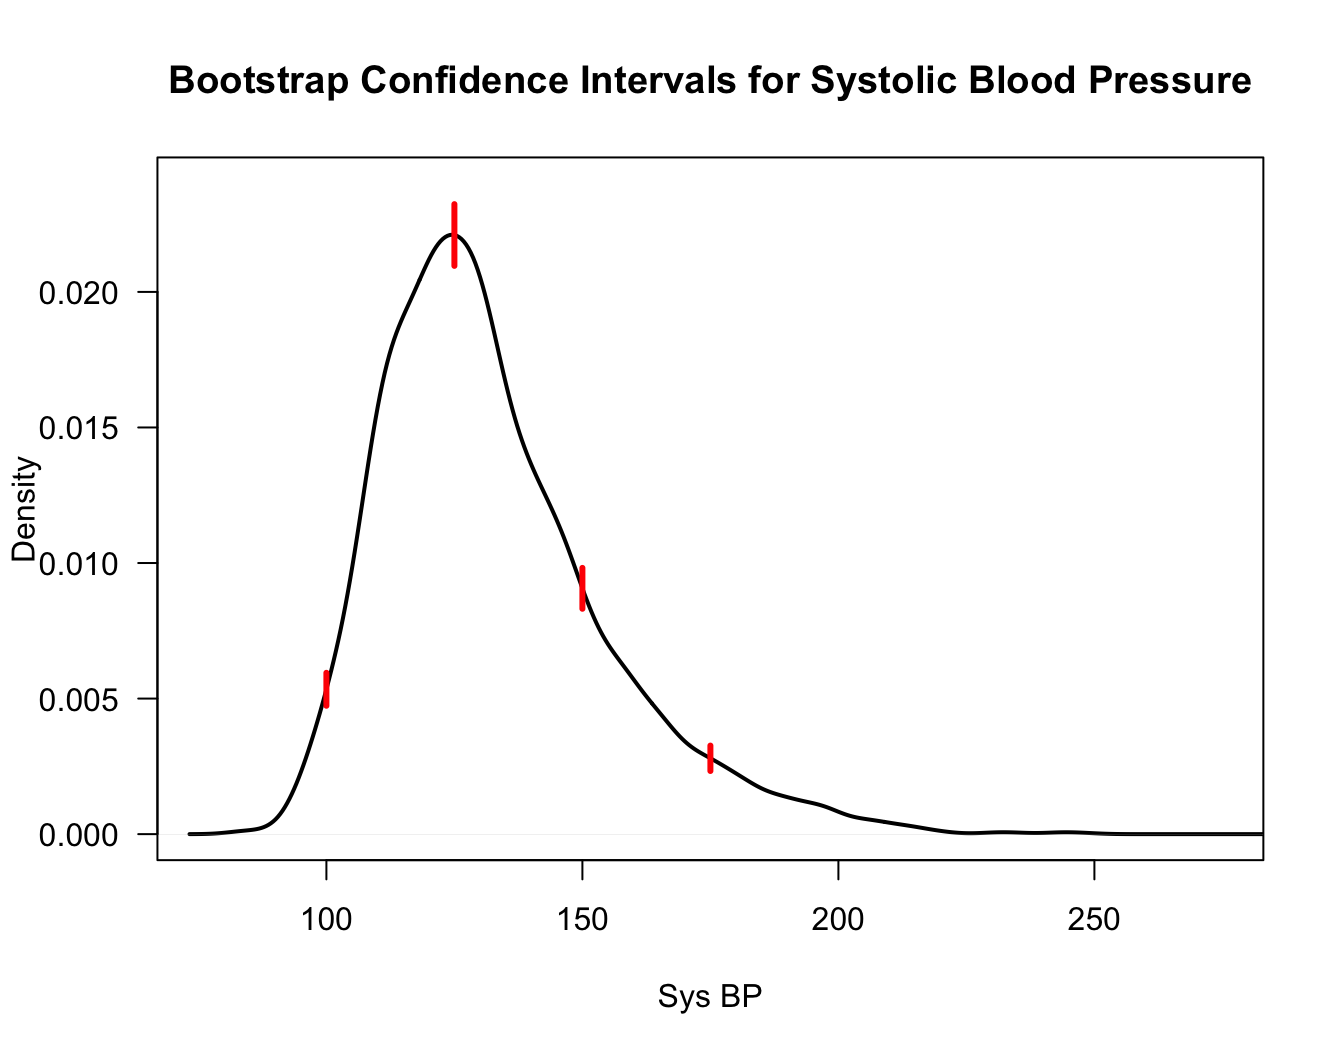
\includegraphics{03-rankstatLatex_files/figure-latex/unnamed-chunk-21-1.pdf} 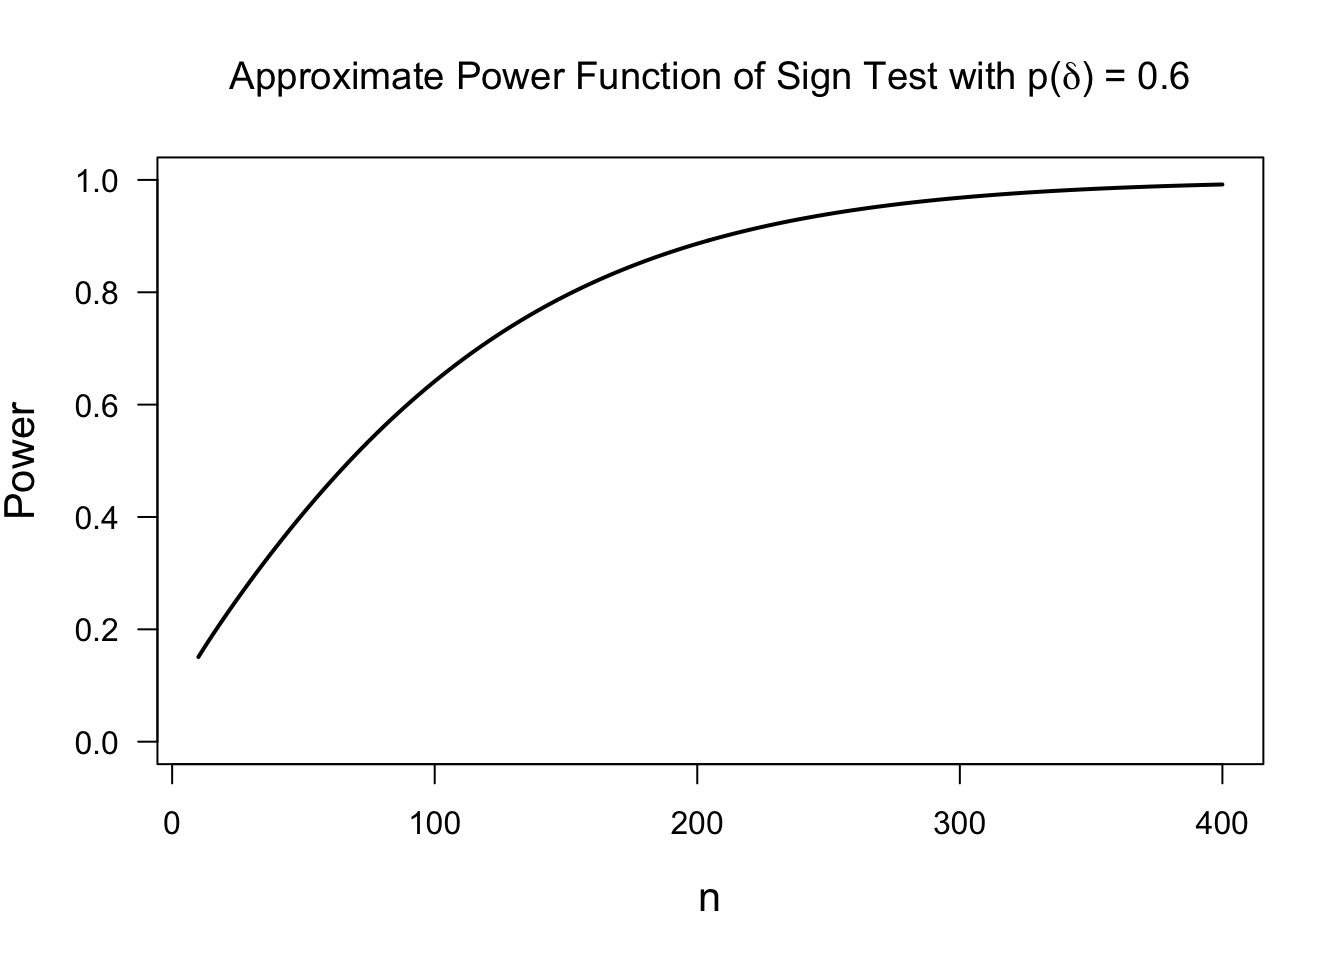
\includegraphics{03-rankstatLatex_files/figure-latex/unnamed-chunk-21-2.pdf}

\begin{center}\rule{0.5\linewidth}{\linethickness}\end{center}

\textbf{Exercise 3.7}: Derive the formula for \(c_{\alpha, n}\) shown in \eqref{eq:critical-value-signstat}.

\begin{center}\rule{0.5\linewidth}{\linethickness}\end{center}

\hypertarget{power-comparisons-and-asymptotic-relative-efficiency}{%
\subsection{Power Comparisons and Asymptotic Relative Efficiency}\label{power-comparisons-and-asymptotic-relative-efficiency}}

\begin{itemize}
\item
  Notice that for the sign statistic power function shown in \eqref{eq:powerfn-signstat},
  we have that
  \begin{equation}
  \lim_{n \longrightarrow \infty} \gamma_{n}(\delta)
  = \begin{cases}
  \alpha & \textrm{ if } \delta = 0 \\
  1 & \textrm{ if } \delta > 0
  \end{cases}
  \label{eq:powerfn-consistent}
  \end{equation}
\item
  The above type of limit for the power function is will be
  true for most ``reasonable'' tests.
\item
  Indeed, a test whose power function satisfies
  \eqref{eq:powerfn-consistent} is typically called a \textbf{consistent} tests.
\end{itemize}

\begin{center}\rule{0.5\linewidth}{\linethickness}\end{center}

\begin{itemize}
\item
  If nearly all reasonable tests are consistent, then
  how can we compare tests with respect to their power?
\item
  One approach is to use simulations to compare power for several plausible alternatives.
  While this can be useful for a specific application, it limits
  our ability to make more general statements about power comparisons.
\item
  Another approach might be to determine
  for which values of \((\delta, n)\) one test has
  greater power than another. However, this could
  be tough to interpret (no test will be uniformly more powerful for all distributions)
  or even difficult to compute.
\item
  One way to think about power is to think about the \textbf{relative efficiency} of
  two testing procedures. The efficiency of a test in this context is
  the sample size required to achieve a certain level of power.
\end{itemize}

\begin{center}\rule{0.5\linewidth}{\linethickness}\end{center}

\begin{itemize}
\item
  To find the asymptotic relative efficiency, we first need to derive the
  asymptotic power function.
\item
  For our hypothesis \(H_{0}: \theta = \theta_{0}\) vs. \(H_{A}: \theta > \theta_{0}\), this is defined as
  \begin{equation}
  \tilde{\gamma}(\delta) = \lim_{n \longrightarrow \infty} \gamma_{n}( \theta_{0} + \delta/\sqrt{n}) \nonumber
  \end{equation}
\item
  Considering the sequence of ``local alternatives'' \(\theta_{n} = \theta_{0} + \delta/\sqrt{n}\),
  we avoid the problem of the power always converging to \(1\).
\item
  It can be shown that
  \begin{equation}
  \tilde{\gamma}(\delta) = 1 - \Phi\Bigg( z_{1-\alpha} - \delta \frac{\mu'(\theta_{0})}{\sigma(\theta_{0})} \Bigg)
  \end{equation}
  as long as we can find functions \(\mu(\cdot)\) and \(\sigma(\cdot)\) such that
  \begin{equation}
  \frac{\sqrt{n}(V_{n} - \mu(\theta_{n}))}{ \sigma(\theta_{n})} \longrightarrow \textrm{Normal}(0, 1) 
  \label{eq:asymptotic-v}
  \end{equation}
  where the test of \(H_{0}:\theta = \theta_{0}\) vs. \(H_{A}: \theta > \theta_{0}\)
  is based on the test statistic \(V_{n}\) with rejection of \(H_{0}\) occurring whenever \(V_{n} \geq c_{\alpha, n}\).
  Statement \eqref{eq:asymptotic-v} asssumes that the distribution of \(V_{n}\) is governed by \(\theta_{n}\) for each \(n\).
\end{itemize}

\begin{center}\rule{0.5\linewidth}{\linethickness}\end{center}

\begin{itemize}
\item
  The ratio \(e(\theta_{0}) = \mu'(\theta_{0})/\sigma(\theta_{0})\) is the \textbf{asymptotic efficiency} of the
  test.
\item
  When comparing two tests with efficiency \(e_{1}(\theta_{0})\) and \(e_{2}(\theta_{0})\),
  the asymptotic relative efficiency of test 1 vs.~test 2 is defined as
  \begin{equation}
  ARE_{12}(\theta_{0}) = \Big( \frac{e_{1}(\theta_{0})}{e_{2}(\theta_{0})} \Big)^{2}
  \end{equation}
\end{itemize}

\begin{center}\rule{0.5\linewidth}{\linethickness}\end{center}

\textbf{Interpretation of Asymptotic Efficiency of Tests}

\begin{itemize}
\item
  Roughly speaking, the asymptotic relative efficiency \(ARE_{12}( \theta_{0} )\) approximately equals
  \(n_{2}/n_{1}\) where \(n_{1}\) is the sample size needed for test 1
  to achieve power \(\beta\) and \(n_{2}\) is the sample size needed for test 2
  to achieve power \(\beta\). This is true for an arbitrary \(\beta\).
\item
  To further justify this interpretation notice that, for large \(n\), we should have
  \begin{equation}
  c_{\alpha, n} \approx \mu(\theta_{0}) + \frac{ \sigma(\theta_{0})z_{1-\alpha}  }{\sqrt{n}}
  \end{equation}
  (This approximation for \(c_{\alpha, n}\) comes from the asymptotic statement in \eqref{eq:asymptotic-v})
\item
  Now, consider the power for detecting \(H_{A}: \theta = \theta_{A}\) (where we will assume
  that \(\theta_{A}\) is ``close'' to \(\theta_{0}\)). Using \eqref{eq:asymptotic-v},
  the approximate power in this setting is
  \begin{eqnarray}
  P_{\theta_{A}}\Big( V_{n} \geq c_{\alpha, n} \Big)
  &=& P_{\theta_{A} }\Bigg( \frac{\sqrt{n}(V_{n} - \mu(\theta_{A} ))}{ \sigma(\theta_{A} )}
  \geq \frac{\sqrt{n}(c_{\alpha,n} - \mu(\theta_{A}))}{ \sigma(\theta_{A})} \Bigg)
  \approx 1 - \Phi\Bigg( \frac{\sqrt{n}(c_{\alpha,n} - \mu(\theta_{A}))}{ \sigma(\theta_{A})} \Bigg)
  \nonumber \\
  &=& 1 - \Phi\Bigg( \frac{\sqrt{n}(\mu(\theta_{0}) - \mu(\theta_{A}))}{ \sigma(\theta_{A})} + \frac{z_{1-\alpha}\sigma(\theta_{0})}{ \sigma(\theta_{A})}\Bigg)
  \end{eqnarray}
\item
  Hence, if we want to achieve a power level of \(\beta\) for the alternative \(H_{A}: \theta = \theta_{A}\),
  we need the corresponding sample size \(n_{\beta}( \theta_{A} )\) to satisfy
  \begin{equation}
  \frac{\sqrt{n_{\beta}(\theta_{A})}(\mu(\theta_{0}) - \mu(\theta_{A}))}{ \sigma(\theta_{A})} + \frac{z_{1-\alpha}\sigma(\theta_{0})}{ \sigma(\theta_{A})}
  = z_{1-\beta}
  \end{equation}
  which reduces to
  \begin{equation}
  n_{\beta}(\theta_{A})
  = \Bigg( \frac{ z_{1-\beta}\sigma(\theta_{A}) - z_{1-\alpha}\sigma(\theta_{0}) }{ \mu(\theta_{0}) - \mu(\theta_{A}) } \Bigg)^{2}
  \approx \Bigg( \frac{ [z_{1-\beta} - z_{1-\alpha}]\sigma(\theta_{0}) }{ (\theta_{A} - \theta_{0})\mu'(\theta_{0})} \Bigg)^{2}
  \label{eq:approx-sample-size}
  \end{equation}
\item
  So, if we were comparing two testing procedures and we computed the approximate sample sizes \(n_{\beta}^{1}(\theta_{A})\) and \(n_{\beta}^{2}(\theta_{A})\) needed to reach \(\beta\) power for the alternative \(H_{A}: \theta = \theta_{A}\), the sample
  size ratio (using approximation \eqref{eq:approx-sample-size}) would be
  \begin{equation}
  \frac{ n_{\beta}^{2}(\theta_{A}) }{n_{\beta}^{1}(\theta_{A}) }
  = \Bigg( \frac{ \mu_{1}'(\theta_{0})\sigma_{2}(\theta_{0}) }{ \mu_{2}'(\theta_{0})\sigma_{1}(\theta_{0})} \Bigg)^{2}
  = \textrm{ARE}_{12}(\theta_{0}) 
  \end{equation}
\item
  Notice that \(\textrm{ARE}_{12}(\theta_{0}) > 1\) indicates that the test \(1\) is better than test \(2\)
  because the sample size required for test \(1\) would be less than the sample size required for test \(2\).
\item
  It is also worth noting that our justification for the interpretation of \(\textrm{ARE}_{12}(\theta_{0})\)
  was not very rigorous or precise, but it is possible to make a more rigorous statement.
  See, for example, Chapter 13 of \citet{lehmann2006} for a more rigorous treatment of relative efficiency.
\item
  In \citet{lehmann2006}, they have a result that states (under appropriate assumptions) that
  \begin{equation}
  \lim_{\theta \downarrow \theta_{0}} \frac{N_{2}(\theta)}{N_{1}(\theta)} 
  = ARE_{12}(\theta_{0})
  \end{equation}
  where \(N_{1}(\theta)\) and \(N_{2}(\theta)\) are the sample
  sizes required to have power \(\beta\) against alternative \(\theta\).
\end{itemize}

\begin{center}\rule{0.5\linewidth}{\linethickness}\end{center}

\hypertarget{efficiency-examples}{%
\subsection{Efficiency Examples}\label{efficiency-examples}}

\textbf{The Sign Test}

\begin{itemize}
\item
  Let us return to the example of the sign statistic \(S_{n}\) and its use
  in testing the hypothesis \(H_{0}: \theta = 0\) vs. \(H_{A}: \theta > 0\).
\item
  Notice that the sign test rejects \(H_{0}:\theta=0\) for \(V_{n} > c_{\alpha,n}\)
  where \(V_{n} = S_{n}/n\) and \(S_{n}\) is the sign statistic.
\item
  When \(V_{n}\) is defined this way \eqref{eq:asymptotic-v} is satisfied
  when \(\mu(\theta) = p(\theta)\) and \(\sigma(\theta) = \sqrt{p(\theta)(1 - p(\theta) )}\)
  where \(p(\theta) = 1 - F_{\epsilon}( -\theta )\).
\item
  Thus, the efficiency of the sign test for testing \(H_{0}: \theta = 0\) vs. \(H_{A}: \theta > 0\) is
  \begin{equation}
  \frac{\mu'(0)}{\sigma(0)} = \frac{p'(0)}{\sqrt{p(0)(1 - p(0))}} = 2f_{\epsilon}(0)
  \end{equation}
  where \(f_{\epsilon}(t) = F_{\epsilon}'(t)\).
\end{itemize}

\begin{center}\rule{0.5\linewidth}{\linethickness}\end{center}

\textbf{The One-Sample t-test}

\begin{itemize}
\item
  Assume that we have data \(D_{1}, \ldots, D_{n}\) generated under the same assumption
  as in our discussion of the sign test and the Wilcoxon signed-rank test. That is,
  \begin{equation}
  D_{i} = \theta + \varepsilon_{i},
  \end{equation}
  where \(\varepsilon_{i}\) are assumed to have median \(0\) with \(\varepsilon_{i}\) having p.d.f. \(f_{\varepsilon}\)
\item
  The one-sample t-test will reject \(H_{0}: \theta = 0\) whenever
  \(V_{n} > c_{\alpha, n}\), where \(V_{n}\) is defined to be
  \begin{equation}
  V_{n} = \frac{\bar{D}}{ \hat{\sigma} }
  \end{equation}
\item
  Note that \eqref{eq:asymptotic-v} will apply if we choose
  \begin{eqnarray}
  \mu(\theta) &=& E_{\theta}(D_{i}) = \theta \nonumber \\
  \sigma(\theta) &=& \sqrt{\textrm{Var}_{\theta}(D_{i})} = \sqrt{\textrm{Var}(\varepsilon_{i})} = \sigma_{\epsilon}
  \end{eqnarray}
\item
  These choices of \(\mu(\theta)\) and \(\sigma(\theta)\) work because
  \begin{eqnarray}
  \frac{\sqrt{n}(V_{n} - \mu(\theta_{n}))}{\sigma(\theta_{n})}
  &=& \frac{\sqrt{n}(\bar{D} - \theta_{n})}{\sigma_{e}} + \sqrt{n}\theta_{n}\Big( \frac{1}{\hat{\sigma}} - \frac{1}{\sigma_{e}}  \Big) \nonumber \\
  &=& \frac{\sqrt{n}(\bar{D} - \theta_{n})}{\sigma_{e}} + \delta\Big( \frac{1}{\hat{\sigma}} - \frac{1}{\sigma_{e}}  \Big)  \nonumber \\
  &\longrightarrow& \textrm{Normal}(0, 1)
  \end{eqnarray}
\item
  So, the efficiency of the one-sample t-test is given by
  \begin{equation}
  \frac{\mu'(0)}{\sigma(0)} = \frac{1}{ \sigma_{e} }  \nonumber 
  \end{equation}
\end{itemize}

\begin{center}\rule{0.5\linewidth}{\linethickness}\end{center}

\textbf{The Wilcoxon Rank Sum Test}

\begin{itemize}
\item
  Using the close relation between the WRS test statistic and
  the Mann-Whitney statistic, the WRS test can be represented as
  rejecting \(H_{0}\) when \(V_{N} \geq c_{\alpha, N}\) where \(V_{N}\) is
  \begin{equation}
  V_{N} = \frac{1}{mn} \sum_{i=1}^{n}\sum_{j=1}^{m} I(X_{i} \geq Y_{j})
  \end{equation}
  and \(N = n + m\).
\item
  The power of the WRS test is usually analyzed in the context of
  the ``shift alternative''. Namely, we are assuming that \(F_{X}(t) = F_{Y}(t - \theta)\)
  and test \(H_{0}: \theta=0\) vs. \(H_{A}: \theta > 0\).
\item
  The natural choice for \(\mu(\theta)\) is the expectation of \(V_{N}\) when \(\theta\) is the true
  shift parameter.
\item
  So, let \(\mu(\theta) = P_{\theta}(X_{i} \geq Y_{j})\). This can be written in terms of \(F_{Y}\) and \(f_{Y}\):
  \begin{eqnarray}
  \mu(\theta) &=& \int_{-\infty}^{\infty} P_{\theta}( X_{i} \geq Y_{j} | Y_{j}=t) f_{Y}(t) dt
  = \int_{-\infty}^{\infty} P_{\theta}( X_{i} \geq t) f_{Y}(t) dt  \nonumber \\
  &=& \int_{-\infty}^{\infty} \{1 - F_{X}(t) \} f_{Y}(t) dt
  = 1 - \int_{-\infty}^{\infty} F_{Y}(t - \theta) f_{Y}(t) dt
  \end{eqnarray}
\item
  You can show that \eqref{eq:asymptotic-v} holds (see e.g, Chapter 14 of \citet{van2000})
  if you choose \(\sigma^{2}(\theta)\) to be
  \begin{eqnarray}
  \sigma^{2}(\theta) &=& \frac{1}{1 - \lambda}\textrm{Var}\{ F_{Y}(X_{i}) \} + \frac{1}{\lambda} \textrm{Var}\{ F_{Y}(Y_{i} - \theta) \}
  \end{eqnarray}
  Here, \(n/(m + n) \longrightarrow \lambda\).
\item
  Thus, the efficiency of testing \(H_{0}: \theta = 0\) for the WRS test is
  \begin{equation}
  e(0) = \frac{\mu'(0)}{\sigma(0)} = \frac{\int_{-\infty}^{\infty} f^{2}(t) dt}{\sigma(0)}
  \end{equation}
\end{itemize}

\hypertarget{efficiency-comparisons-for-several-distributions}{%
\subsection{Efficiency Comparisons for Several Distributions}\label{efficiency-comparisons-for-several-distributions}}

\textbf{Sign Test vs.~One-Sample t-test}

\begin{itemize}
\item
  Comparisons of the Efficiency of the sign and one-sample t-test only
  require us to find \(f_{\epsilon}(0)\) and \(\sigma_{e}^{2}\) for different assumptions
  about the residual density \(f_{\epsilon}\).
\item
  For the Logistic(0,1) distribution, \(f_{\epsilon}(0) = 1/4\) and the standard deviation
  is \(\pi/\sqrt{3}\). Hence, the asymptotic relative efficiency of the sign test vs.~the one-sample
  t-test would be \((\pi/2\sqrt{3})^{2}\).
\item
  The relative efficiencies for the sign vs.~t-test for other distributions are shown below
  \begin{eqnarray}
  \textrm{Distribution} & & \quad \textrm{Efficiency} \\
  \textrm{Normal}(0,1) & & \qquad 2/\pi \\
  \textrm{Logistic}(0,1) & &  \qquad \pi^{2}/12 \\
  \textrm{Laplace}(0,1) & & \qquad 2 \\
  \textrm{Uniform}(-1, 1) & & \qquad 1/3 \\
  \textrm{t-dist}_{\nu} & & \qquad [4(\nu/(\nu-2))\Gamma^{2}\{ (\nu + 1)/2\}]/[ \Gamma^{2}(\nu/2)\nu \pi ]
  \end{eqnarray}
\end{itemize}

\begin{center}\rule{0.5\linewidth}{\linethickness}\end{center}

\textbf{WRS Test vs.~Two-Sample t-test}

\begin{itemize}
\tightlist
\item
  The relative efficiencies for the WRS test vs.~the two-sample t-test
  for several distributions are shown below.
\end{itemize}

\begin{eqnarray}
\textrm{Distribution} & & \quad \textrm{Efficiency} \\
\textrm{Normal}(0,1) & & \qquad 3/\pi \\
\textrm{Logistic}(0,1) & &  \qquad \pi^{2}/9 \\
\textrm{Laplace}(0,1) & & \qquad 3/2 \\
\textrm{Uniform}(-1, 1) & & \qquad 1 \\
\textrm{t-dist}_{3} & & \qquad 1.24 \\
\textrm{t-dist}_{5} & & \qquad 1.90 \\
\end{eqnarray}

\hypertarget{a-power-contest}{%
\subsection{A Power ``Contest''}\label{a-power-contest}}

\begin{itemize}
\item
  To compare power across for specific sample sizes, effect sizes, and
  distributional assumptions, a simulation study can be more
  helpful than statements about asymptotic relative efficiency.
\item
  Below shows the results of a simulation study in \textbf{R} which compares
  power for the one-sample testing problem.
\item
  This simulation study compares the sign test, Wilcoxon signed rank test,
  and the one-sample t-test.
\item
  It is assumed that \(n = 200\) and that responses \(D_{i}\) are generated from
  the following model:
  \begin{equation}
  D_{i} = 0.2 + \varepsilon_{i}
  \end{equation}
\item
  Three choices for the distribution of \(\varepsilon_{i}\) were considered:

  \begin{itemize}
  \tightlist
  \item
    \(\varepsilon_{i} \sim \textrm{Logistic}(0, 1)\)
  \item
    \(\varepsilon_{i} \sim \textrm{Normal}(0, 1)\)
  \item
    \(\varepsilon_{i} \sim \textrm{Uniform}(-3/2, 3/2)\)
  \end{itemize}
\item
  The \textbf{R} code and simulation results are shown below.
\end{itemize}

\begin{Shaded}
\begin{Highlighting}[]
\KeywordTok{set.seed}\NormalTok{(}\DecValTok{148930}\NormalTok{)}
\NormalTok{theta <-}\StringTok{ }\FloatTok{0.2}
\NormalTok{n <-}\StringTok{ }\DecValTok{200}
\NormalTok{nreps <-}\StringTok{ }\DecValTok{500}
\NormalTok{RejectSign <-}\StringTok{ }\NormalTok{RejectWilcoxonSign <-}\StringTok{ }\NormalTok{RejectT <-}\StringTok{ }\KeywordTok{matrix}\NormalTok{(}\OtherTok{NA}\NormalTok{, }\DataTypeTok{nrow=}\NormalTok{nreps, }\DataTypeTok{ncol=}\DecValTok{4}\NormalTok{)}
\ControlFlowTok{for}\NormalTok{(k }\ControlFlowTok{in} \DecValTok{1}\OperatorTok{:}\NormalTok{nreps) \{}
\NormalTok{  xx <-}\StringTok{ }\NormalTok{theta }\OperatorTok{+}\StringTok{ }\KeywordTok{rlogis}\NormalTok{(n)}
\NormalTok{  yy <-}\StringTok{ }\NormalTok{theta }\OperatorTok{+}\StringTok{ }\KeywordTok{rnorm}\NormalTok{(n)}
\NormalTok{  zz <-}\StringTok{ }\NormalTok{theta }\OperatorTok{+}\StringTok{ }\KeywordTok{runif}\NormalTok{(n, }\DataTypeTok{min=}\OperatorTok{-}\DecValTok{3}\OperatorTok{/}\DecValTok{2}\NormalTok{, }\DataTypeTok{max=}\DecValTok{3}\OperatorTok{/}\DecValTok{2}\NormalTok{)}
\NormalTok{  ww <-}\StringTok{ }\NormalTok{theta }\OperatorTok{+}\StringTok{ }\NormalTok{(}\KeywordTok{rexp}\NormalTok{(n, }\DataTypeTok{rate=}\DecValTok{1}\NormalTok{) }\OperatorTok{-}\StringTok{ }\KeywordTok{rexp}\NormalTok{(n, }\DataTypeTok{rate=}\DecValTok{1}\NormalTok{))}\OperatorTok{/}\KeywordTok{sqrt}\NormalTok{(}\DecValTok{2}\NormalTok{)}
  
\NormalTok{  RejectSign[k,}\DecValTok{1}\NormalTok{] <-}\StringTok{ }\KeywordTok{ifelse}\NormalTok{(}\KeywordTok{binom.test}\NormalTok{(}\DataTypeTok{x=}\KeywordTok{sum}\NormalTok{(xx }\OperatorTok{>}\StringTok{ }\DecValTok{0}\NormalTok{), }\DataTypeTok{n=}\NormalTok{n, }\DataTypeTok{p=}\FloatTok{0.5}\NormalTok{)}\OperatorTok{$}\NormalTok{p.value }\OperatorTok{<}\StringTok{ }\FloatTok{0.05}\NormalTok{, }\DecValTok{1}\NormalTok{, }\DecValTok{0}\NormalTok{)}
\NormalTok{  RejectWilcoxonSign[k,}\DecValTok{1}\NormalTok{] <-}\StringTok{ }\KeywordTok{ifelse}\NormalTok{(}\KeywordTok{wilcox.test}\NormalTok{(xx)}\OperatorTok{$}\NormalTok{p.value }\OperatorTok{<}\StringTok{ }\FloatTok{0.05}\NormalTok{, }\DecValTok{1}\NormalTok{, }\DecValTok{0}\NormalTok{) }
\NormalTok{  RejectT[k,}\DecValTok{1}\NormalTok{] <-}\StringTok{ }\KeywordTok{ifelse}\NormalTok{(}\KeywordTok{t.test}\NormalTok{(xx)}\OperatorTok{$}\NormalTok{p.value }\OperatorTok{<}\StringTok{ }\FloatTok{0.05}\NormalTok{, }\DecValTok{1}\NormalTok{, }\DecValTok{0}\NormalTok{)}
  
\NormalTok{  RejectSign[k,}\DecValTok{2}\NormalTok{] <-}\StringTok{ }\KeywordTok{ifelse}\NormalTok{(}\KeywordTok{binom.test}\NormalTok{(}\DataTypeTok{x=}\KeywordTok{sum}\NormalTok{(yy }\OperatorTok{>}\StringTok{ }\DecValTok{0}\NormalTok{), }\DataTypeTok{n=}\NormalTok{n, }\DataTypeTok{p=}\FloatTok{0.5}\NormalTok{)}\OperatorTok{$}\NormalTok{p.value }\OperatorTok{<}\StringTok{ }\FloatTok{0.05}\NormalTok{, }\DecValTok{1}\NormalTok{, }\DecValTok{0}\NormalTok{)}
\NormalTok{  RejectWilcoxonSign[k,}\DecValTok{2}\NormalTok{] <-}\StringTok{ }\KeywordTok{ifelse}\NormalTok{(}\KeywordTok{wilcox.test}\NormalTok{(yy)}\OperatorTok{$}\NormalTok{p.value }\OperatorTok{<}\StringTok{ }\FloatTok{0.05}\NormalTok{, }\DecValTok{1}\NormalTok{, }\DecValTok{0}\NormalTok{) }
\NormalTok{  RejectT[k,}\DecValTok{2}\NormalTok{] <-}\StringTok{ }\KeywordTok{ifelse}\NormalTok{(}\KeywordTok{t.test}\NormalTok{(yy)}\OperatorTok{$}\NormalTok{p.value }\OperatorTok{<}\StringTok{ }\FloatTok{0.05}\NormalTok{, }\DecValTok{1}\NormalTok{,}\DecValTok{0}\NormalTok{)  }
  
\NormalTok{  RejectSign[k,}\DecValTok{3}\NormalTok{] <-}\StringTok{ }\KeywordTok{ifelse}\NormalTok{(}\KeywordTok{binom.test}\NormalTok{(}\DataTypeTok{x=}\KeywordTok{sum}\NormalTok{(zz }\OperatorTok{>}\StringTok{ }\DecValTok{0}\NormalTok{), }\DataTypeTok{n=}\NormalTok{n, }\DataTypeTok{p=}\FloatTok{0.5}\NormalTok{)}\OperatorTok{$}\NormalTok{p.value }\OperatorTok{<}\StringTok{ }\FloatTok{0.05}\NormalTok{, }\DecValTok{1}\NormalTok{, }\DecValTok{0}\NormalTok{)}
\NormalTok{  RejectWilcoxonSign[k,}\DecValTok{3}\NormalTok{] <-}\StringTok{ }\KeywordTok{ifelse}\NormalTok{(}\KeywordTok{wilcox.test}\NormalTok{(zz)}\OperatorTok{$}\NormalTok{p.value }\OperatorTok{<}\StringTok{ }\FloatTok{0.05}\NormalTok{, }\DecValTok{1}\NormalTok{, }\DecValTok{0}\NormalTok{) }
\NormalTok{  RejectT[k,}\DecValTok{3}\NormalTok{] <-}\StringTok{ }\KeywordTok{ifelse}\NormalTok{(}\KeywordTok{t.test}\NormalTok{(zz)}\OperatorTok{$}\NormalTok{p.value }\OperatorTok{<}\StringTok{ }\FloatTok{0.05}\NormalTok{,}\DecValTok{1}\NormalTok{,}\DecValTok{0}\NormalTok{)  }
  
\NormalTok{  RejectSign[k,}\DecValTok{4}\NormalTok{] <-}\StringTok{ }\KeywordTok{ifelse}\NormalTok{(}\KeywordTok{binom.test}\NormalTok{(}\DataTypeTok{x=}\KeywordTok{sum}\NormalTok{(ww }\OperatorTok{>}\StringTok{ }\DecValTok{0}\NormalTok{), }\DataTypeTok{n=}\NormalTok{n, }\DataTypeTok{p=}\FloatTok{0.5}\NormalTok{)}\OperatorTok{$}\NormalTok{p.value }\OperatorTok{<}\StringTok{ }\FloatTok{0.05}\NormalTok{, }\DecValTok{1}\NormalTok{, }\DecValTok{0}\NormalTok{)}
\NormalTok{  RejectWilcoxonSign[k,}\DecValTok{4}\NormalTok{] <-}\StringTok{ }\KeywordTok{ifelse}\NormalTok{(}\KeywordTok{wilcox.test}\NormalTok{(ww)}\OperatorTok{$}\NormalTok{p.value }\OperatorTok{<}\StringTok{ }\FloatTok{0.05}\NormalTok{, }\DecValTok{1}\NormalTok{, }\DecValTok{0}\NormalTok{) }
\NormalTok{  RejectT[k,}\DecValTok{4}\NormalTok{] <-}\StringTok{ }\KeywordTok{ifelse}\NormalTok{(}\KeywordTok{t.test}\NormalTok{(ww)}\OperatorTok{$}\NormalTok{p.value }\OperatorTok{<}\StringTok{ }\FloatTok{0.05}\NormalTok{, }\DecValTok{1}\NormalTok{, }\DecValTok{0}\NormalTok{)}
\NormalTok{\}}

\NormalTok{power.results <-}\StringTok{ }\KeywordTok{data.frame}\NormalTok{(}\DataTypeTok{Distribution=}\KeywordTok{c}\NormalTok{(}\StringTok{"Logistic"}\NormalTok{, }\StringTok{"Normal"}\NormalTok{, }\StringTok{"Uniform"}\NormalTok{, }\StringTok{"Laplace"}\NormalTok{),}
                 \DataTypeTok{SignTest=}\KeywordTok{colMeans}\NormalTok{(RejectSign), }\DataTypeTok{WilcoxonSign=}\KeywordTok{colMeans}\NormalTok{(RejectWilcoxonSign),}
                 \DataTypeTok{tTest=}\KeywordTok{colMeans}\NormalTok{(RejectT))}
\end{Highlighting}
\end{Shaded}

\begin{table}[ht]
\centering
\begin{tabular}{cccc}
  \hline
Distribution & SignTest & WilcoxonSign & tTest \\ 
  \hline
Logistic & 0.25 & 0.37 & 0.34 \\ 
  Normal & 0.59 & 0.77 & 0.81 \\ 
  Uniform & 0.44 & 0.87 & 0.90 \\ 
  Laplace & 0.93 & 0.92 & 0.81 \\ 
   \hline
\end{tabular}
\caption{Estimated power for three one-sample tests and
              three distributions. 500 simulation replications were used.} 
\end{table}

\hypertarget{linear-rank-statistics-in-general}{%
\section{Linear Rank Statistics in General}\label{linear-rank-statistics-in-general}}

\hypertarget{definition-1}{%
\subsection{Definition}\label{definition-1}}

\begin{itemize}
\item
  The Wilcoxon rank sum statistic is an example of a statistic from a more general class of rank statistics.
\item
  This is the class of \textbf{linear rank statistics}.
\item
  Suppose we have observations \(\mathbf{Z} = (Z_{1}, \ldots, Z_{N})\).
  A linear rank statistic is a statistic \(T_{N}\) that can be expressed as
  \begin{equation}
  T_{N} = \sum_{i=1}^{N} c_{iN} a_{N}\big( R_{i}( \mathbf{Z} ) \big)
  \label{eq:general-linear-rank}
  \end{equation}
\item
  The terms \(c_{1N}, \ldots, c_{NN}\) are usually called \textbf{coefficients}. These
  are fixed numbers and are not random variables.
\item
  The terms \(a_{N}(R_{i}( \mathbf{Z} ) )\) are commonly referred to as \textbf{scores}.
\item
  Typically, the scores are generated from a given function \(\psi\) in
  the following way
  \begin{equation}
  a_{N}(i) = \psi\Big( \frac{i}{N+1} \Big) 
  \end{equation}
\end{itemize}

\begin{center}\rule{0.5\linewidth}{\linethickness}\end{center}

\textbf{Example: WRS statistic }

\begin{itemize}
\item
  For the Wilcoxon rank sum test, we separated the data \(\mathbf{Z} = (Z_{1}, \ldots, Z_{N})\)
  into two groups.
\item
  The first \(n\) observations were from group 1 while the
  last \(m\) observations were from group 2.
\item
  The WRS statistic was then defined as
  \begin{equation}
  W = \sum_{i=1}^{n} R_{i}(\mathbf{Z})
  \end{equation}
\item
  In this case, the WRS statistic can be expressed in the form \eqref{eq:general-linear-rank}
  if we choose the coefficients to be the following
  \begin{equation}
  c_{iN} = \begin{cases}
   1 & \textrm{ if } i \leq n \\
   0 & \textrm{ if } i > n 
   \end{cases}
  \end{equation}
  and we choose the scores to be
  \begin{equation}
  a_{N}(i) = i
  \end{equation}
\end{itemize}

\hypertarget{properties-of-linear-rank-statistics}{%
\subsection{Properties of Linear Rank Statistics}\label{properties-of-linear-rank-statistics}}

\begin{itemize}
\item
  The expected value of the linear rank statistic (if the distribution of the \(Z_{i}\) is continuous)
  is
  \begin{equation}
  E(T_{N}) = N\bar{c}_{N}\bar{a}_{N},
  \label{eq:expec-linear-rank}
  \end{equation}
  where \(\bar{c}_{N} = \frac{1}{N} \sum_{j=1}^{N} c_{jN}\) and \(\bar{a}_{N} = \frac{1}{N}\sum_{j=1}^{N} a_{N}(j)\)
\item
  The formula \eqref{eq:expec-linear-rank} for the expectation only uses the fact that \(R_{i}(\mathbf{Z})\) has a discrete uniform
  distribution. So,
  \begin{equation}
  E\{ a_{N}( R_{i}(\mathbf{Z} ) \}
  = \sum_{j=1}^{N} a_{N}(j)P\{ R_{i}( \mathbf{Z}) = j \}
  = \sum_{j=1}^{N} \frac{ a_{N}(j) }{N}
  = \bar{a}_{N}
  \end{equation}
  Using this, we can then see that
  \begin{equation}
  E( T_{N} ) = \sum_{j=1}^{N} c_{jN} E\{ a_{N}(R_{i}(\mathbf{Z})) \}
  = \sum_{j=1}^{N} c_{jN}\bar{a}_{N} = N\bar{c}_{N}\bar{a}_{N}
  \end{equation}
\end{itemize}

\begin{center}\rule{0.5\linewidth}{\linethickness}\end{center}

\begin{itemize}
\tightlist
\item
  A similar argument can show that the variance of \(T_{N}\) is
  \begin{equation}
  \textrm{Var}( T_{N} ) = \frac{N^{2}}{n-1} \sigma_{a}^{2}\sigma_{c}^{2},
  \end{equation}
  where \(\sigma_{c}^{2} = \frac{1}{N}\sum_{j=1}^{N} (c_{jN} - \bar{c}_{N})^{2}\)
  and \(\sigma_{a}^{2} = \frac{1}{N}\sum_{j=1}^{N} (a_{N}(j) - \bar{a}_{N})^{2}\)
\end{itemize}

\begin{center}\rule{0.5\linewidth}{\linethickness}\end{center}

\begin{itemize}
\item
  To perform hypothesis testing when using a general linear rank statistics,
  working with the exact distribution or performing permutation tests can
  often be computationally demanding.
\item
  Using a large-sample approximation is often easier.
\item
  As long as a few conditions for the coefficients and scores are satisfied,
  one can state the following
  \begin{equation}
  \frac{T_{N} - E( T_{N})}{\sqrt{\textrm{Var}(T_{N})}} \longrightarrow \textrm{Normal}(0, 1),
  \end{equation}
  where, as we showed, both \(E(T_{N})\) and \(\textrm{Var}(T_{N})\) both have closed-form expressions
  for an arbitrary linear rank statistic.
\end{itemize}

\hypertarget{other-examples-of-linear-rank-statistics}{%
\subsection{Other Examples of Linear Rank Statistics}\label{other-examples-of-linear-rank-statistics}}

\hypertarget{the-van-der-waerden-statistic-and-the-normal-scores-test}{%
\subsubsection{The van der Waerden statistic and the normal scores test}\label{the-van-der-waerden-statistic-and-the-normal-scores-test}}

\begin{itemize}
\item
  Van der Waerden's rank statistic is used for two-sample problems
  where the first \(n\) observations come from group 1 while the last
  \(m\) observations come from group 2.
\item
  Van der Waerden's rank statistic \(VW_{N}\) is defined as
  \begin{equation}
  VW_{N} = \sum_{j=1}^{n} \Phi^{-1}\Bigg( \frac{\mathbf{R}_{i}( \mathbf{Z})}{N+1} \Bigg)
  \end{equation}
\item
  The function \(\Phi^{-1}\) denotes the inverse of the cumulative distribution
  function of a standard Normal random variable.
\item
  The statistic \(VW_{N}\) is a linear rank statistic with coefficients
  \begin{equation}
  c_{iN} = \begin{cases}
   1 & \textrm{ if } i \leq n \\
   0 & \textrm{ if } i > n 
   \end{cases}
  \end{equation}
  and scores determined by
  \begin{equation}
  a_{N}(i) = \Phi^{-1}\Big(  \frac{i}{N+1} \Big)
  \end{equation}
\item
  A test based on van der Waerden's statistic is often referred to as
  the \textbf{normal scores test}.
\item
  The normal scores test is often suggested as an attractive test when
  the underlying data has an approximately normal distribution.
\item
  If you plot a histogram of the van der Waerden scores \(a_{N}(i)\) it should look
  roughly like a Gaussian distribution (if there are not too many ties).
\end{itemize}

\hypertarget{the-median-test}{%
\subsubsection{The median test}\label{the-median-test}}

\begin{itemize}
\item
  The median test is also a two-sample rank test.
\item
  While the Wilcoxon rank sum test looks at the average rank within group \(1\),
  the median test instead looks at how many of the ranks from group \(1\)
  are less than the median rank (which should equal \((N+1)/2\)).
\item
  The test statistic \(M_{N}\) for the median test is defined as
  \begin{equation}
  M_{N} = \sum_{i=1}^{n} I\Big( R_{i}(\mathbf{Z}) \leq \frac{N+1}{2} \Big)
  \end{equation}
  because \((N+1)/2\) will be the median rank.
\item
  This is a linear rank statistic with coefficients
  \begin{equation}
  c_{iN} = \begin{cases}
   1 & \textrm{ if } i \leq n \\
   0 & \textrm{ if } i > n 
   \end{cases}
  \end{equation}
  and scores
  \begin{equation}
  a_{N}(i) = 
  \begin{cases}
   1 & \textrm{ if } i \leq (N+1)/2 \\
   0 & \textrm{ if } i > (N+1)/2 
   \end{cases}
  \end{equation}
\item
  The median test could be used to test whether or not observations
  from group 1 tend to be smaller than those from group 2.
\end{itemize}

\hypertarget{choosing-the-scores-a_ni}{%
\subsection{\texorpdfstring{Choosing the scores \(a_{N}(i)\)}{Choosing the scores a\_\{N\}(i)}}\label{choosing-the-scores-a_ni}}

\begin{itemize}
\item
  The rank tests we have discussed so far are nonparametric in the sense
  that their null distribution does not depend on any particular parametric
  assumptions about the distributions from which the observations arise.
\item
  For power calculations, we often think of some parameter or ``effect size''
  modifying the base distribution in some way.
\item
  For example, we often think of the shift alternative \(F_{X}(t) = F_{Y}(t - \theta)\)
  in the two-sample problem.
\end{itemize}

\begin{center}\rule{0.5\linewidth}{\linethickness}\end{center}

\begin{itemize}
\item
  In parametric statistics, when testing \(H_{0}:\theta = 0\) the most powerful test
  of \(H_{0}: \theta = \theta_{0}\) vs. \(H_{A}:\theta = \theta_{A}\) is based on
  rejecting \(H_{0}\) whenever the likelihood ratio is large enough:
  \begin{equation}
  \textrm{Reject } H_{0} \textrm{ if: } \quad \frac{p_{\theta_{A}}(\mathbf{z})}{p_{\theta_{0}}(\mathbf{z})} \geq c_{\alpha, n}
  \label{eq:parametric-np-lemma}
  \end{equation}
  This is the Neyman-Pearson Lemma.
\item
  The same property is true if we are considering tests based on ranks. The most powerful test
  for testing \(H_{0}: \theta = \theta_{0}\) vs. \(H_{A}:\theta = \theta_{A}\) is based on
  \begin{equation}
  \textrm{Reject } H_{0} \textrm{ if: } \quad 
  \frac{P_{\theta_{A}}\Big( R_{1}(\mathbf{Z}), \ldots, R_{N}(\mathbf{Z}) \Big)}{ P_{\theta_{0}}\Big( R_{1}(\mathbf{Z}), \ldots, R_{N}(\mathbf{Z}) \Big) } \geq c_{\alpha, n}
  \label{eq:nonparametric-np-lemma}
  \end{equation}
\item
  The main difference between \eqref{eq:parametric-np-lemma} and \eqref{eq:parametric-np-lemma} is
  that the distribution \(P_{\theta_{A}}\Big( R_{1}(\mathbf{Z}), \ldots, R_{N}(\mathbf{Z}) \Big)\)
  is unknown unless we are willing to make certain distributional assumptions.
\item
  Nevertheless, we can approximate this probability if \(\theta_{A}\) is a location parameter ``close'' to \(\theta_{0}\)
\end{itemize}

\begin{equation}
P_{\theta_{A}}\Big( R_{1}(\mathbf{Z}), \ldots, R_{N}(\mathbf{Z}) \Big)
\approx P_{\theta_{0}}\Big( R_{1}(\mathbf{Z}), \ldots, R_{N}(\mathbf{Z}) \Big)
+ \frac{\theta_{A}}{N!}\sum_{i=1}^{N} c_{iN} E\Bigg\{ \frac{\partial \log f(Z_{(i)})}{ \partial Z}  \Bigg\}
\end{equation}

where \(Z_{(i)}\) denotes the \(i^{th}\) order statistic.
See, for example, Chapter 13 of \citet{van2000} for more details on the derivation of this approximation.

\begin{itemize}
\item
  So, large values of the linear rank statistic \(T_{N} = \sum_{i=1}^{N} c_{iN} a_{N}(i)\) will approximately
  correspond to large values of \(P_{\theta_{A}}\Big( R_{1}(\mathbf{Z}), \ldots, R_{N}(\mathbf{Z}) \Big)\)
  if we choose the scores to be
  \begin{equation}
  a_{N}(i) = E\Bigg\{ \frac{\partial \log f(Z_{(i)})}{ \partial Z}  \Bigg\}
  \end{equation}
\item
  Linear rank statistics with scores generated this way are usually called
  \textbf{locally most powerful} rank test.
\end{itemize}

\begin{center}\rule{0.5\linewidth}{\linethickness}\end{center}

\begin{itemize}
\item
  The best choice of the scores will depend on what we assume about the density \(f\).
\item
  For example, if we assume that \(f(z)\) is \(\textrm{Normal}(0,1)\), then
  \begin{equation}
  \frac{\partial \log f(z)}{\partial z} = -z
  \end{equation}
\item
  The approximate expectation of the order statistics from a Normal\((0,1)\) distribution are
  \begin{equation}
  E\{ Z_{(i)} \} \approx \Phi^{-1}\Bigg( \frac{i}{N+1} \Bigg)
  \end{equation}
  This implies that the van der Waerden's scores are approximately optimal
  if we assume the distribution of the \(Z_{i}\) is Normal.
\item
  This can also be worked out for other choices of \(f(z)\).
\item
  If \(f(z)\) is a Logistic distribution, the optimal scores correspond to the Wilcoxon rank sum test statistic.
\item
  If \(f(z)\) is Laplace (meaning that \(f(z) = \frac{1}{2}e^{-|z|}\)), then the optimal scores
  correspond to the median test.
\end{itemize}

\hypertarget{additional-reading}{%
\section{Additional Reading}\label{additional-reading}}

\begin{itemize}
\tightlist
\item
  Additional reading which covers the material discussed in this chapter includes:

  \begin{itemize}
  \tightlist
  \item
    Chapters 3-4 from \citet{hollander2013}
  \end{itemize}
\end{itemize}

\hypertarget{krusk-wallis}{%
\chapter{Rank Tests for Multiple Groups}\label{krusk-wallis}}

\begin{itemize}
\item
  We can roughly think of the tests discussed in Chapter 3
  as being related to the well-known parametric tests shown in the table below.
  \begin{eqnarray}
  \textbf{Parametric Test} & & \qquad  \textbf{ Nonparametric Tests } \nonumber \\
      & & \nonumber \\
  \textrm{One-Sample t-test} & & \qquad  \textrm{Wilcoxon Signed Rank/Sign Test} \nonumber \\
  \textrm{Two-Sample t-test} & & \qquad \textrm{Wilcoxon Rank Sum/Normal Scores/Median Test} \nonumber
  \end{eqnarray}
\item
  The \textbf{Kruskal-Wallis} test can be though of as the
  nonparametric analogue of one-way analysis of variance (ANOVA).
\item
  For \(K \geq 3\) groups, one-way ANOVA considers the analysis of observations
  arising from the following model
  \begin{equation}
  Y_{kj} = \mu_{k} + \varepsilon_{kj}, \qquad j=1,\ldots, n_{k}; k=1,\ldots,K  
  \label{eq:normal-anova-model}
  \end{equation}
  where it is often assumed that \(\varepsilon_{kj} \sim \textrm{Normal}(0, \sigma^{2})\).
\item
  Usually, the one-way ANOVA hypothesis of interest is something like
  \begin{equation}
  H_{0}: \mu_{1} = \mu_{2} = \ldots = \mu_{K}
  \label{eq:homogeneity-hyp}
  \end{equation}
  which is often referred to as the homogeneity hypothesis.
\item
  A test of the hypothesis \eqref{eq:homogeneity-hyp} is based on decomposing the observed variation in
  the responses \(Y_{kj}\):
  \begin{eqnarray}
  \underbrace{ \sum_{k=1}^{K}\sum_{j=1}^{n_{k}} (Y_{kj} - \bar{Y}_{..})^{2}}_{SST} &=& \sum_{k=1}^{K}\sum_{j=1}^{n_{k}} (\bar{Y}_{k.} - \bar{Y}_{..})^{2} + \sum_{k=1}^{K}\sum_{j=1}^{n_{k}} (Y_{kj} - \bar{Y}_{k.})^{2} \nonumber \\
  &=& \underbrace{\sum_{k=1}^{K} n_{k} (\bar{Y}_{k.} - \bar{Y}_{..})^{2}}_{SSA} + \underbrace{\sum_{k=1}^{K}\sum_{j=1}^{n_{k}} (Y_{kj} - \bar{Y}_{k.})^{2}}_{SSE} 
  \label{eq:anova-decomp}
  \end{eqnarray}
  where \(\bar{Y}_{k.} = \frac{1}{n_{k}}\sum_{j=1}^{n_{k}} Y_{kj}\) and \(\bar{Y}_{..} = \frac{1}{K}\sum_{k=1}^{K} \bar{Y}_{k.}\).
\item
  Large values of \(SSA = \sum_{k=1}^{K} n_{k} (\bar{Y}_{k.} - \bar{Y}_{..})^{2}\) provide evidence against the null hypothesis \eqref{eq:homogeneity-hyp}. The alternative hypothesis here is that there is at least one pair of means \(\mu_{h}, \mu_{l}\)
  such that \(\mu_{h} \neq \mu_{l}\).
\end{itemize}

\hypertarget{the-kruskal-wallis-test}{%
\section{The Kruskal-Wallis Test}\label{the-kruskal-wallis-test}}

\hypertarget{definition-2}{%
\subsection{Definition}\label{definition-2}}

\begin{itemize}
\item
  Instead of assuming \eqref{eq:normal-anova-model} for the responses \(Y_{kj}\), a nonparametric way of thinking
  about this problem is to instead only assume that
  \begin{equation}
  Y_{kj} \sim F_{k}
  \end{equation}
  That is, \(Y_{k1}, Y_{k2}, \ldots, Y_{kn_{k}}\) is an i.i.d. sample from \(F_{k}\) for each \(k\).
\item
  A nonparametric version of the one-way ANOVA homogeneity hypothesis is
  \begin{equation}
  H_{0}: F_{1} = F_{2} = \ldots = F_{K}
  \label{eq:nonpar-homogeneity-hyp}
  \end{equation}
\item
  The ``shift alternative'' in this case can be stated as
  \begin{equation}
  H_{A}: F_{k}(t) = F(t - \Delta_{k}), \quad \textrm{ for } k = 1, \ldots K \quad \textrm{ and not all $\Delta_{k}$ equal}
  \end{equation}
\end{itemize}

\begin{center}\rule{0.5\linewidth}{\linethickness}\end{center}

\begin{itemize}
\item
  The \textbf{Kruskal-Wallis test statistic} \(KW_{N}\) is similar to the SSA term (defined in \eqref{eq:anova-decomp})
  in the one-way ANOVA setting.
\item
  Rather than comparing the group-specific means \(\bar{Y}_{k.}\) with the overall mean \(\bar{Y}_{..}\),
  the Kruskal-Wallis test statistic compares the group-specific rank
  means \(\bar{R}_{k.}\) with their overall expectation under the null hypothesis.
\item
  The Kruskal-Wallis test statistic is defined as
  \begin{equation}
  KW_{N} = \frac{12}{N(N-1)}\sum_{k=1}^{K} n_{k}\Big( \bar{R}_{k.} - \frac{N + 1}{2} \Big)^{2}, \quad \textrm{ where } N = \sum_{k=1}^{K} n_{k}
  \label{eq:kw-definition}
  \end{equation}
\item
  In \eqref{eq:kw-definition}, \(\bar{R}_{k.}\) is the average rank of those in the \(k^{th}\) group
  \begin{equation}
  \bar{R}_{k.} = \frac{1}{n_{k}} \sum_{j=1}^{n_{k}} R_{kj}(\mathbf{Z}),
  \end{equation}
  where \(\mathbf{Z}\) denotes the pooled-data vector and \(R_{kj}(\mathbf{Z})\) denotes
  the rank of \(Y_{kj}\) in the ``pooled-data ranking''.
\end{itemize}

\begin{center}\rule{0.5\linewidth}{\linethickness}\end{center}

\begin{itemize}
\item
  What is the expectation of \(\bar{R}_{k.}\) under the null hypothesis \eqref{eq:nonpar-homogeneity-hyp}?
\item
  Again, if the null hypothesis is true, we can treat all of our responses \(Y_{kj}\) as just
  an i.i.d. sample of size \(N\) from a common distribution function \(F\).
\item
  Hence, as we showed in \eqref{eq:rank-expectation} from Chapter 3, \(E\{ R_{kj}(\mathbf{Z}) \} = (N+1)/2\) under the
  assumption that the data are an i.i.d. sample from a common distribution function.
\item
  So, the intuition behind the definition of \(KW_{N}\) is that the differences
  \(\bar{R}_{k.} - \frac{N + 1}{2}\) should be small whenever the homogeneity
  hypothesis \eqref{eq:nonpar-homogeneity-hyp} is true.
\end{itemize}

\begin{center}\rule{0.5\linewidth}{\linethickness}\end{center}

\begin{itemize}
\item
  When \(K=2\), the following relationship between the Kruskal-Wallis statistic
  \(KW_{N}\) and the Wilcoxon rank sum test statistic \(W\) from Chapter 3 holds.
  \begin{equation}
  KW_{N} = \frac{12}{mn(N+1)}\Big( W - \frac{n(N+1)}{2}  \Big)^{2}.
  \label{eq:kw-wrs-equivalence}
  \end{equation}
\item
  Hence, the p-value from a Kruskal-Wallis test and a (two-sided)
  WRS test should be the same when \(K = 2\).
\item
  However, you cannot directly perform a one-sided test using
  the Kruskal-Wallis test.
\end{itemize}

\begin{center}\rule{0.5\linewidth}{\linethickness}\end{center}

\begin{itemize}
\tightlist
\item
  \textbf{Exercise 4.1} If \(K=2\), show that equation \eqref{eq:kw-wrs-equivalence} holds.
\end{itemize}

\begin{center}\rule{0.5\linewidth}{\linethickness}\end{center}

\textbf{An Example}

\begin{table}[ht]
\centering
\begin{tabular}{ccc}
  \hline
Group & Y & Rank \\ 
  \hline
Group 1 & 1.00 & 8 \\ 
  Group 1 & -1.20 & 2 \\ 
  Group 1 & -1.50 & 1 \\ 
  Group 2 & 0.00 & 5 \\ 
  Group 2 & -0.10 & 4 \\ 
  Group 2 & 1.10 & 9 \\ 
  Group 3 & 0.90 & 7 \\ 
  Group 3 & -0.40 & 3 \\ 
  Group 3 & 0.60 & 6 \\ 
   \hline
\end{tabular}
\end{table}

\begin{itemize}
\tightlist
\item
  Consider the data shown in the table. In this case, \(N = 9\), \(\bar{R}_{1.} = 11/3\), \(\bar{R}_{2.} = 6\), and \(\bar{R}_{3.} = 16/3\). The Kruskall-Wallis
  statistic is
  \begin{equation}
  KW_{N} = \frac{1}{2}\Big\{ 3(11/3 - 5)^{2} + 3(6 - 5)^{2} + 3(16/3 - 5)^{2}   \Big\} = 13/9  \nonumber
  \end{equation}
\end{itemize}

\hypertarget{asymptotic-distribution-and-connection-to-one-way-anova}{%
\subsection{Asymptotic Distribution and Connection to One-Way ANOVA}\label{asymptotic-distribution-and-connection-to-one-way-anova}}

\begin{itemize}
\item
  The Kruskal-Wallis statistic \(KW_{N}\) has
  an asymptotic chi-square distribution with \(K-1\) degrees of freedom under the null hypothesis \eqref{eq:nonpar-homogeneity-hyp}.
\item
  This follows from the fact that \((\bar{R}_{k.} - (N+1)/2)\) is approximately normally distributed
  for large \(n_{k}\).
\item
  \textbf{R} uses the large-sample approximation when computing
  the p-value for the Kruskal-Wallis test.
\end{itemize}

\begin{center}\rule{0.5\linewidth}{\linethickness}\end{center}

\begin{itemize}
\item
  The Kruskal-Wallis test can also be thought of as the test you would obtain
  if you applied the one-way ANOVA setup to the ranks of \(Y_{kj}\).
\item
  The one-way ANOVA test is based on the value of SSA where, as in \eqref{eq:anova-decomp},
  SSA is defined as
  \begin{equation}
  SSA = \sum_{k=1}^{K} n_{k} (\bar{Y}_{k.} - \bar{Y}_{..})^{2} \nonumber
  \end{equation}
\item
  You then reject \(H_{0}\), when \(SSA/SSE = SSA/(SST - SSA)\) is sufficiently large.
\item
  Notice that if we computed SSA using the ranks \(R_{kj}( \mathbf{Z} )\)
  rather than the observations \(Y_{kj}\), we would get:
  \begin{eqnarray}
  SSA_{r} &=& \sum_{k=1}^{K} n_{k} \Big( \bar{R}_{k.} - \bar{R}_{..} \Big)^{2}  \nonumber \\
  &=& \sum_{k=1}^{K} n_{k} (\bar{R}_{k.} - \frac{N+1}{2})^{2}  \nonumber \\
  &=& \frac{N(N-1)}{12} KW_{N}  
  \label{eq:ssa-kw}
  \end{eqnarray}
\item
  If you were applying ANOVA to the ranks of \(Y_{kj}\), \(SST_{r}\) would be
  the following fixed constant:
  \begin{equation}
  \textrm{SST}_{r} = \frac{N(N + 1)(N-1)}{12} \nonumber
  \end{equation}
\item
  So, any test of the homogeneity hypothesis would
  be based on just the value of \(SSA_{r}\) which, as we showed in \eqref{eq:ssa-kw},
  is just a constant times the Kruskal-Wallis statistic.
\end{itemize}

\hypertarget{performing-the-kruskal-wallis-test-in-r}{%
\section{Performing the Kruskal-Wallis Test in R}\label{performing-the-kruskal-wallis-test-in-r}}

\begin{itemize}
\tightlist
\item
  We will look at performing Kruskal-Wallis tests in \textbf{R} by using the
  ``InsectSprays'' dataset.
\end{itemize}

\begin{Shaded}
\begin{Highlighting}[]
\KeywordTok{head}\NormalTok{(InsectSprays)}
\end{Highlighting}
\end{Shaded}

\begin{verbatim}
##   count spray
## 1    10     A
## 2     7     A
## 3    20     A
## 4    14     A
## 5    14     A
## 6    12     A
\end{verbatim}

\begin{itemize}
\item
  This dataset has 72 observations.
\item
  The variable \textbf{count} is the number of
  insects measured in some agricultural unit.
\item
  The variable \textbf{spray} was the type of spray used on
  that unit.
\item
  You could certainly argue that a standard ANOVA is not
  appropriate in this situation because the responses are counts,
  and for count data, the variance is usually a function of the mean.
\item
  A generalized linear model with a log link function might be more appropriate.
\item
  Applying a square-root transformation to count data is also a commonly suggested
  approach. (The square-root transformation is the ``variance-stabilizing transformation''
  for Poisson-distributed data).
\end{itemize}

\begin{Shaded}
\begin{Highlighting}[]
\KeywordTok{boxplot}\NormalTok{(}\KeywordTok{sqrt}\NormalTok{(count) }\OperatorTok{~}\StringTok{ }\NormalTok{spray, }\DataTypeTok{data=}\NormalTok{InsectSprays,}\DataTypeTok{las=}\DecValTok{1}\NormalTok{, }
        \DataTypeTok{ylab=}\StringTok{"square root of insect counts"}\NormalTok{)}
\end{Highlighting}
\end{Shaded}

\includegraphics{04-multistatLatex_files/figure-latex/unnamed-chunk-2-1.pdf}

\begin{center}\rule{0.5\linewidth}{\linethickness}\end{center}

\begin{itemize}
\tightlist
\item
  Let us perform a test of homogeneity using both the one-way ANOVA approach and a Kruskal-Wallis
  test
\end{itemize}

\begin{Shaded}
\begin{Highlighting}[]
\KeywordTok{anova}\NormalTok{(}\KeywordTok{lm}\NormalTok{(}\KeywordTok{sqrt}\NormalTok{(count) }\OperatorTok{~}\StringTok{ }\NormalTok{spray, }\DataTypeTok{data=}\NormalTok{InsectSprays))}
\end{Highlighting}
\end{Shaded}

\begin{verbatim}
## Analysis of Variance Table
## 
## Response: sqrt(count)
##           Df Sum Sq Mean Sq F value    Pr(>F)    
## spray      5 88.438 17.6876  44.799 < 2.2e-16 ***
## Residuals 66 26.058  0.3948                      
## ---
## Signif. codes:  0 '***' 0.001 '**' 0.01 '*' 0.05 '.' 0.1 ' ' 1
\end{verbatim}

\begin{Shaded}
\begin{Highlighting}[]
\NormalTok{a  <-}\StringTok{ }\KeywordTok{kruskal.test}\NormalTok{(}\KeywordTok{sqrt}\NormalTok{(count) }\OperatorTok{~}\StringTok{ }\NormalTok{spray, }\DataTypeTok{data=}\NormalTok{InsectSprays)}
\NormalTok{a}\OperatorTok{$}\NormalTok{p.value}
\end{Highlighting}
\end{Shaded}

\begin{verbatim}
## [1] 1.510844e-10
\end{verbatim}

\begin{center}\rule{0.5\linewidth}{\linethickness}\end{center}

\begin{itemize}
\tightlist
\item
  Notice that applying the square root transformation does not affect the
  value of the Kruskal-Wallis statistic or the Kruskal-Wallis p-value.
\end{itemize}

\begin{Shaded}
\begin{Highlighting}[]
\KeywordTok{kruskal.test}\NormalTok{(count }\OperatorTok{~}\StringTok{ }\NormalTok{spray, }\DataTypeTok{data=}\NormalTok{InsectSprays)}
\end{Highlighting}
\end{Shaded}

\begin{verbatim}
## 
##  Kruskal-Wallis rank sum test
## 
## data:  count by spray
## Kruskal-Wallis chi-squared = 54.691, df = 5, p-value = 1.511e-10
\end{verbatim}

\begin{itemize}
\tightlist
\item
  This invariance to data transformation is not true for the standard one-way ANOVA.
\end{itemize}

\begin{Shaded}
\begin{Highlighting}[]
\KeywordTok{anova}\NormalTok{(}\KeywordTok{lm}\NormalTok{(count }\OperatorTok{~}\StringTok{ }\NormalTok{spray, }\DataTypeTok{data=}\NormalTok{InsectSprays))}
\end{Highlighting}
\end{Shaded}

\begin{verbatim}
## Analysis of Variance Table
## 
## Response: count
##           Df Sum Sq Mean Sq F value    Pr(>F)    
## spray      5 2668.8  533.77  34.702 < 2.2e-16 ***
## Residuals 66 1015.2   15.38                      
## ---
## Signif. codes:  0 '***' 0.001 '**' 0.01 '*' 0.05 '.' 0.1 ' ' 1
\end{verbatim}

\hypertarget{comparison-of-specific-groups}{%
\section{Comparison of Specific Groups}\label{comparison-of-specific-groups}}

\begin{itemize}
\item
  A Kruskal-Wallis test performs a test of the overall homogeneity hypothesis
  \begin{equation}
  H_{0}: F_{1} = F_{2} = \ldots = F_{K}
  \end{equation}
\item
  However, a rejection of the homogeneity hypothesis does not indicate which
  group differences are primarily the source of this rejection nor
  does it provide any measure of the ``magnitude'' of the differences between
  each of the groups.
\item
  Dunn's test is the suggested way to compute pairwise tests of stochatic dominance.
\item
  Performing a series of pairwise Wilcoxon rank sum test can
  lead to violations of transitivity. For example,
  group A is ``better'' than B which is better than C, but
  group C is better than A.
\item
  In \textbf{R}, Dunn's test can be performed using the \textbf{dunn.test} package.
\end{itemize}

\begin{center}\rule{0.5\linewidth}{\linethickness}\end{center}

\begin{itemize}
\item
  In traditional one-way ANOVA one often reports pairwise differences
  in the means and their associated confidence intervals.
\item
  In the context of a Kruskal-Wallis test, one could
  report pairwise differences in the Hodges-Lehmann estimate
  though other comparisons may also be of interest.
\item
  One nice approach is to use the proportional odds model
  interpretation of the Kruskal-Wallis test and
  then report the difference in the estimated proportional odds coefficients.
  See Section 7.6 of \url{http://hbiostat.org/doc/bbr.pdf} for more details
  on the proportional odds model.
\end{itemize}

\includegraphics{04-multistatLatex_files/figure-latex/unnamed-chunk-7-1.pdf}

\hypertarget{an-additional-example}{%
\section{An Additional Example}\label{an-additional-example}}

\begin{itemize}
\tightlist
\item
  We will use the ``cane'' dataset from the \textbf{boot} package.
\end{itemize}

\begin{Shaded}
\begin{Highlighting}[]
\KeywordTok{library}\NormalTok{(boot)}
\KeywordTok{data}\NormalTok{(cane)}
\KeywordTok{head}\NormalTok{(cane)}
\end{Highlighting}
\end{Shaded}

\begin{verbatim}
##     n  r  x var block
## 1  87 76 19   1     A
## 2 119  8 14   2     A
## 3  94 74  9   3     A
## 4  95 11 12   4     A
## 5 134  0 12   5     A
## 6  92  0  3   6     A
\end{verbatim}

\begin{itemize}
\item
  These data come from a study trying to determine the susceptibility of different types
  of sugar cane to a particular type of disease.
\item
  The variable \textbf{n} contains the total number of shoots in each plot.
\item
  The variable \textbf{r} containes the total number of diseased shoots.
\item
  We can create a new variable \textbf{prop} that measures the proportion
  of shoots that are diseased.
\end{itemize}

\begin{Shaded}
\begin{Highlighting}[]
\NormalTok{cane}\OperatorTok{$}\NormalTok{prop <-}\StringTok{ }\NormalTok{cane}\OperatorTok{$}\NormalTok{r}\OperatorTok{/}\NormalTok{cane}\OperatorTok{$}\NormalTok{n}
\end{Highlighting}
\end{Shaded}

\begin{itemize}
\tightlist
\item
  You could certainly argue that a logistic regression model is a better approach here,
  but we will analyze the transformed proportions using the arcsine square root transformation.
\end{itemize}

\begin{Shaded}
\begin{Highlighting}[]
\NormalTok{cane}\OperatorTok{$}\NormalTok{prop.trans <-}\StringTok{ }\KeywordTok{asin}\NormalTok{(}\KeywordTok{sqrt}\NormalTok{(cane}\OperatorTok{$}\NormalTok{prop))}
\KeywordTok{boxplot}\NormalTok{(prop.trans }\OperatorTok{~}\StringTok{ }\NormalTok{block, }\DataTypeTok{data=}\NormalTok{cane, }\DataTypeTok{las=}\DecValTok{1}\NormalTok{, }\DataTypeTok{ylab=}\StringTok{"number of shoots"}\NormalTok{)}
\end{Highlighting}
\end{Shaded}

\includegraphics{04-multistatLatex_files/figure-latex/unnamed-chunk-10-1.pdf}

\begin{Shaded}
\begin{Highlighting}[]
\KeywordTok{kruskal.test}\NormalTok{(prop }\OperatorTok{~}\StringTok{ }\NormalTok{block, }\DataTypeTok{data=}\NormalTok{cane)}
\end{Highlighting}
\end{Shaded}

\begin{verbatim}
## 
##  Kruskal-Wallis rank sum test
## 
## data:  prop by block
## Kruskal-Wallis chi-squared = 1.1355, df = 3, p-value = 0.7685
\end{verbatim}

\hypertarget{additional-reading-1}{%
\section{Additional Reading}\label{additional-reading-1}}

\begin{itemize}
\tightlist
\item
  Additional reading which covers the material discussed in this chapter includes:

  \begin{itemize}
  \tightlist
  \item
    Chapters 6 from \citet{hollander2013}
  \end{itemize}
\end{itemize}

\hypertarget{permutation}{%
\chapter{Permutation Tests}\label{permutation}}

\begin{itemize}
\item
  Permutation tests are a useful tool that allows you to avoid depending on
  specific parametric assumptions.
\item
  Permutation tests are also useful in more complex modern applications where it can be
  difficult to work out the theoretical null distribution of the desired test statistic.
\end{itemize}

\hypertarget{notation}{%
\section{Notation}\label{notation}}

\begin{itemize}
\item
  A \textbf{permutation} \(\pi\) of a set \(S\) is a function \(\pi: S \longrightarrow S\) is a
  function that is both one-to-one and onto.
\item
  We will usually think of \(S\) as the set of observation indices in which case
  \(S = \{1, \ldots, N\}\) for sample size \(N\).
\item
  Each permutation \(\pi\) of \(S = \{1, \ldots, N\}\) defines a particular ordering of the elements of \(S\).
  For this reason, a permutation is often expressed as the following ordered list
  \begin{equation}
  \pi = \big( \pi(1), \pi(2), \ldots, \pi(N)  \big) \nonumber 
  \end{equation}
\item
  In other words, we can think of a permutation of \(S\)
  as a particular ordering of the elements of \(S\).
\item
  For example, if \(S = \{1,2,3\}\), and \(\pi_{1}\) is a permutation of \(S\)
  defined as \(\pi_{1}(1) = 3\), \(\pi_{1}(2) = 1\), \(\pi_{1}(3) = 2\), then
  this permutation expressed as an ordered list would be
  \begin{equation}
  \pi_{1} = (3, 1, 2)  \nonumber
  \end{equation}
\item
  There are \(5\) other possible permutations of \(S\):
  \begin{eqnarray}
  \pi_{2} &=& (1,2,3) \nonumber \\
  \pi_{3} &=& (2,1,3) \nonumber \\
  \pi_{4} &=& (1,3,2) \nonumber \\
  \pi_{5} &=& (3,2,1) \nonumber \\
  \pi_{6} &=& (2, 3, 1) \nonumber  
  \end{eqnarray}
\item
  If \(S\) has \(N\) distinct elements, there are \(N!\) possible permutations of \(S\).
\item
  We will let \(\mathcal{S}_{N}\) denote the set of all permutations of the
  set \(\{1, \ldots, N\}\).
\end{itemize}

\hypertarget{permutation-tests-for-the-two-sample-problem}{%
\section{Permutation Tests for the Two-Sample Problem}\label{permutation-tests-for-the-two-sample-problem}}

\begin{itemize}
\tightlist
\item
  Permutation tests for two-sample problems are motivated by the following reasoning:

  \begin{itemize}
  \tightlist
  \item
    If there is no real difference between the two groups,
    there is nothing ``special'' about the difference in means
    between the two groups.
  \item
    The observed difference in the mean between the two groups
    should not be notably different than mean differences from
    randomly formed groups.
  \item
    Forming ``random'' groups can be done by using many permutations
    of the original data.
  \end{itemize}
\end{itemize}

\hypertarget{example-1}{%
\subsection{Example 1}\label{example-1}}

\begin{itemize}
\item
  Suppose we have observations from two groups \(X_{1}, \ldots, X_{n} \sim F_{X}\)
  and \(Y_{1}, \ldots, Y_{m} \sim F_{Y}\).
\item
  Let \(\mathbf{Z} = (Z_{1}, \ldots, Z_{N})\) denote the pooled data
  \begin{equation}
  (Z_{1}, \ldots, Z_{N}) = (X_{1}, \ldots, X_{n}, Y_{1}, \ldots, Y_{m})
  \end{equation}
\item
  For a permutation \(\pi\) of \(\{1, \ldots, N\}\), we will let \(\mathbf{Z}_{\pi}\)
  denote the corresponding permuted dataset
  \begin{equation}
  \mathbf{Z}_{\pi} = (Z_{\pi(1)}, Z_{\pi(2)}, \ldots, Z_{\pi(N)})
  \end{equation}
\end{itemize}

\begin{table}[ht]
\centering
\begin{tabular}{ccccccc}
  \hline
 & OriginalData & Perm1 & Perm2 & Perm3 & Perm4 & Perm5 \\ 
  \hline
z1 & 0.60 & -0.60 & 0.60 & -0.90 & 0.70 & 0.60 \\ 
  z2 & -0.80 & -1.40 & -0.60 & 0.70 & -0.40 & -0.60 \\ 
  z3 & -0.60 & 0.70 & 0.20 & 0.60 & -1.40 & -0.80 \\ 
  z4 & -0.90 & 0.20 & -0.40 & 0.20 & 0.20 & 0.30 \\ 
  z5 & 0.30 & -0.40 & -1.30 & -0.40 & -0.90 & -0.40 \\ 
  z6 & -1.30 & -1.30 & -1.40 & -0.60 & -0.80 & 0.70 \\ 
  z7 & 0.20 & 0.30 & 0.70 & -1.40 & 0.30 & -0.90 \\ 
  z8 & 0.70 & 0.60 & 0.30 & -1.30 & 0.60 & 0.20 \\ 
  z9 & -1.40 & -0.90 & -0.80 & 0.30 & -0.60 & -1.40 \\ 
  z10 & -0.40 & -0.80 & -0.90 & -0.80 & -1.30 & -1.30 \\ 
  mean difference & 0.16 & 0.12 & 0.12 & 0.80 & 0.00 & 0.36 \\ 
   \hline
\end{tabular}
\caption{Example of Permuting a Vector of Responses.
              This example assumes n=m=5.} 
\end{table}

\begin{itemize}
\item
  For example, the columns in Table 5.1 are just permutations of the original data \(\mathbf{Z}\).
\item
  Suppose we want to base a test on the difference in the means between the two groups
  \begin{equation}
  T_{N}(\mathbf{Z}) = \bar{X} - \bar{Y} = \frac{1}{n}\sum_{i=1}^{n} Z_{i} - \frac{1}{m}\sum_{i=n+1}^{N} Z_{i}
  \end{equation}
\item
  We will let \(t_{obs}\) denote the observed value of the mean difference. That is,
  \(t_{obs} = T_{N}(\mathbf{Z}_{obs})\), where \(\mathbf{Z}_{obs}\) is the vector of the observed data.
\item
  Under the null hypothesis that \(F_{X} = F_{Y}\), the observed mean difference
  should not be ``abnormal'' when compared with the mean differences from
  many other permutations of the data.
\end{itemize}

\begin{Shaded}
\begin{Highlighting}[]
\NormalTok{z <-}\StringTok{ }\KeywordTok{c}\NormalTok{(}\FloatTok{0.6}\NormalTok{, }\FloatTok{-0.8}\NormalTok{, }\FloatTok{-0.6}\NormalTok{, }\FloatTok{-0.9}\NormalTok{, }\FloatTok{0.3}\NormalTok{, }\FloatTok{-1.3}\NormalTok{, }\FloatTok{0.2}\NormalTok{, }\FloatTok{0.7}\NormalTok{, }\FloatTok{-1.4}\NormalTok{, }\FloatTok{-0.4}\NormalTok{) }\CommentTok{## data}
\NormalTok{observed.diff <-}\StringTok{ }\KeywordTok{mean}\NormalTok{(z[}\DecValTok{1}\OperatorTok{:}\DecValTok{5}\NormalTok{]) }\OperatorTok{-}\StringTok{ }\KeywordTok{mean}\NormalTok{(z[}\DecValTok{6}\OperatorTok{:}\DecValTok{10}\NormalTok{])  }\CommentTok{## observed mean difference}
\NormalTok{nperms <-}\StringTok{ }\DecValTok{1000}
\NormalTok{mean.diff <-}\StringTok{ }\KeywordTok{rep}\NormalTok{(}\OtherTok{NA}\NormalTok{, nperms)}
\ControlFlowTok{for}\NormalTok{(k }\ControlFlowTok{in} \DecValTok{1}\OperatorTok{:}\NormalTok{nperms) \{}
\NormalTok{    ss <-}\StringTok{ }\KeywordTok{sample}\NormalTok{(}\DecValTok{1}\OperatorTok{:}\DecValTok{10}\NormalTok{, }\DataTypeTok{size=}\DecValTok{10}\NormalTok{)  }\CommentTok{## draw a random permutation}
\NormalTok{    z.perm <-}\StringTok{ }\NormalTok{z[ss]   }\CommentTok{## form the permuted dataset}
\NormalTok{    mean.diff[k] <-}\StringTok{ }\KeywordTok{mean}\NormalTok{(z.perm[}\DecValTok{1}\OperatorTok{:}\DecValTok{5}\NormalTok{]) }\OperatorTok{-}\StringTok{ }\KeywordTok{mean}\NormalTok{(z.perm[}\DecValTok{6}\OperatorTok{:}\DecValTok{10}\NormalTok{]) }\CommentTok{## compute mean difference}
                                                           \CommentTok{## for permuted dataset}
\NormalTok{\}}
\KeywordTok{hist}\NormalTok{(mean.diff, }\DataTypeTok{las=}\DecValTok{1}\NormalTok{, }\DataTypeTok{col=}\StringTok{"grey"}\NormalTok{, }\DataTypeTok{main=}\StringTok{"Permutation Distribution }
\StringTok{     of Mean Difference"}\NormalTok{)}
\KeywordTok{abline}\NormalTok{(}\DataTypeTok{v=}\NormalTok{observed.diff, }\DataTypeTok{lwd=}\DecValTok{3}\NormalTok{)}
\end{Highlighting}
\end{Shaded}

\includegraphics{05-permutationLatex_files/figure-latex/unnamed-chunk-1-1.pdf}

\hypertarget{permutation-test-p-values}{%
\subsection{Permutation Test p-values}\label{permutation-test-p-values}}

\begin{itemize}
\item
  The one-sided p-value for the permutation test is
  \begin{eqnarray}
  \textrm{p-value} &=& \frac{\textrm{number of permutations such that } T_{N} \geq t_{obs}}{ N! } \nonumber \\
  &=& \frac{1}{N!} \sum_{\pi \in \mathcal{S}_{N}} I\Big( T_{N}(\mathbf{Z}_{\pi}) \geq t_{obs} \Big) \nonumber
  \end{eqnarray}
\item
  The two-sided p-value for the two-sample problem would be
  \begin{equation}
  \textrm{p-value} 
  = \frac{1}{N!} \sum_{\pi \in \mathcal{S}_{N}} I\Big( \Big| T_{N}(\mathbf{Z}_{\pi}) \Big|  \geq |t_{obs}| \Big) \nonumber
  \end{equation}
\item
  As we did when producing the above histogram, the permutation-test p-value is
  often computed by using a large number of random permutations rather
  than computing the test statistic for every possible permutation.
\item
  The Monte Carlo permutation-test p-value is defined as
  \begin{equation}
  \textrm{p-value}_{mc} = \frac{1}{S+1}\Bigg[ 1 +  \sum_{s = 1}^{S} I\Big( T_{N}(\mathbf{Z}_{\pi_{s}}) \geq t_{obs} \Big) \Bigg]
  \end{equation}
  where \(\pi_{1}, \ldots, \pi_{S}\) are randomly drawn permutations
\item
  The two-sided (Monte Carlo) p-value for the example shown in Table 5.1 is
\end{itemize}

\begin{Shaded}
\begin{Highlighting}[]
\NormalTok{pval.mc <-}\StringTok{ }\NormalTok{(}\DecValTok{1} \OperatorTok{+}\StringTok{ }\KeywordTok{sum}\NormalTok{(}\KeywordTok{abs}\NormalTok{(mean.diff) }\OperatorTok{>=}\StringTok{ }\KeywordTok{abs}\NormalTok{(observed.diff)))}\OperatorTok{/}\NormalTok{(nperms }\OperatorTok{+}\StringTok{ }\DecValTok{1}\NormalTok{)}
\KeywordTok{round}\NormalTok{(pval.mc, }\DecValTok{2}\NormalTok{)}
\end{Highlighting}
\end{Shaded}

\begin{verbatim}
## [1] 0.77
\end{verbatim}

\hypertarget{example-2-ratios-of-means}{%
\subsection{Example 2: Ratios of Means}\label{example-2-ratios-of-means}}

\begin{itemize}
\item
  With permutation tests, you are not limited to difference in means. You can choose
  the statistic \(T_{N}(\mathbf{Z})\) to measure other contrasts of interest.
\item
  For example, with nonnegative data you might be interested in the ratio of means between the two groups
  \begin{equation}
  T_{N}( \mathbf{Z} ) = \max\Big\{ \bar{X}/\bar{Y} , \bar{Y}/\bar{X}  \Big\}
  \end{equation}
\item
  Let us see how this works for a simulated example with \(n = m = 20\) where we assume that
  \(X_{1}, \ldots, X_{n} \sim \textrm{Exponential}(1)\) and \(Y_{1}, \ldots, Y_{m} \sim \textrm{Exponential}(1/2)\).
\end{itemize}

\begin{Shaded}
\begin{Highlighting}[]
\KeywordTok{set.seed}\NormalTok{(}\DecValTok{5127}\NormalTok{)}
\NormalTok{xx <-}\StringTok{ }\KeywordTok{rexp}\NormalTok{(}\DecValTok{20}\NormalTok{, }\DataTypeTok{rate=}\DecValTok{1}\NormalTok{)}
\NormalTok{yy <-}\StringTok{ }\KeywordTok{rexp}\NormalTok{(}\DecValTok{20}\NormalTok{, }\DataTypeTok{rate=}\FloatTok{0.5}\NormalTok{)}
\NormalTok{zz <-}\StringTok{ }\KeywordTok{c}\NormalTok{(xx, yy) }\CommentTok{## this is the original data}
\NormalTok{t.obs <-}\StringTok{ }\KeywordTok{max}\NormalTok{(}\KeywordTok{mean}\NormalTok{(zz[}\DecValTok{1}\OperatorTok{:}\DecValTok{20}\NormalTok{])}\OperatorTok{/}\KeywordTok{mean}\NormalTok{(zz[}\DecValTok{21}\OperatorTok{:}\DecValTok{40}\NormalTok{]), }\KeywordTok{mean}\NormalTok{(zz[}\DecValTok{21}\OperatorTok{:}\DecValTok{40}\NormalTok{])}\OperatorTok{/}\KeywordTok{mean}\NormalTok{(zz[}\DecValTok{1}\OperatorTok{:}\DecValTok{20}\NormalTok{]))}
\NormalTok{nperms <-}\StringTok{ }\DecValTok{500}
\NormalTok{mean.ratio <-}\StringTok{ }\KeywordTok{rep}\NormalTok{(}\DecValTok{0}\NormalTok{, nperms)}
\ControlFlowTok{for}\NormalTok{(k }\ControlFlowTok{in} \DecValTok{1}\OperatorTok{:}\NormalTok{nperms) \{}
\NormalTok{     ss <-}\StringTok{ }\KeywordTok{sample}\NormalTok{(}\DecValTok{1}\OperatorTok{:}\DecValTok{40}\NormalTok{, }\DataTypeTok{size=}\DecValTok{40}\NormalTok{)}
\NormalTok{     zz.perm <-}\StringTok{ }\NormalTok{zz[ss]}
\NormalTok{     mean.ratio[k] <-}\StringTok{ }\KeywordTok{max}\NormalTok{(}\KeywordTok{mean}\NormalTok{(zz.perm[}\DecValTok{1}\OperatorTok{:}\DecValTok{20}\NormalTok{])}\OperatorTok{/}\KeywordTok{mean}\NormalTok{(zz.perm[}\DecValTok{21}\OperatorTok{:}\DecValTok{40}\NormalTok{]), }
                          \KeywordTok{mean}\NormalTok{(zz.perm[}\DecValTok{21}\OperatorTok{:}\DecValTok{40}\NormalTok{])}\OperatorTok{/}\KeywordTok{mean}\NormalTok{(zz.perm[}\DecValTok{1}\OperatorTok{:}\DecValTok{20}\NormalTok{]))}
\NormalTok{\}}
\KeywordTok{hist}\NormalTok{(mean.ratio, }\DataTypeTok{las=}\DecValTok{1}\NormalTok{, }\DataTypeTok{col=}\StringTok{"grey"}\NormalTok{, }\DataTypeTok{main=}\StringTok{"Permutation Distribution }
\StringTok{     of Maximum Mean Ratio"}\NormalTok{, }\DataTypeTok{xlab=}\StringTok{"maximum mean ratio"}\NormalTok{)}
\KeywordTok{abline}\NormalTok{(}\DataTypeTok{v=}\NormalTok{t.obs, }\DataTypeTok{lwd=}\DecValTok{3}\NormalTok{)}
\end{Highlighting}
\end{Shaded}

\includegraphics{05-permutationLatex_files/figure-latex/unnamed-chunk-3-1.pdf}

\begin{itemize}
\tightlist
\item
  The two-side (Monte Carlo) permutation test p-value is:
\end{itemize}

\begin{Shaded}
\begin{Highlighting}[]
\NormalTok{pval.mc <-}\StringTok{ }\NormalTok{(}\DecValTok{1} \OperatorTok{+}\StringTok{ }\KeywordTok{sum}\NormalTok{(mean.ratio }\OperatorTok{>=}\StringTok{ }\NormalTok{t.obs))}\OperatorTok{/}\NormalTok{(nperms }\OperatorTok{+}\StringTok{ }\DecValTok{1}\NormalTok{)}
\KeywordTok{round}\NormalTok{(pval.mc, }\DecValTok{2}\NormalTok{)}
\end{Highlighting}
\end{Shaded}

\begin{verbatim}
## [1] 0.04
\end{verbatim}

\hypertarget{example-3-differences-in-quantiles}{%
\subsection{Example 3: Differences in Quantiles}\label{example-3-differences-in-quantiles}}

\begin{itemize}
\item
  Permutation tests are especially useful in problems where working out the null distribution
  is difficult, or when certain approximations of the null distributions are hard to justify.
\item
  An example of this occurrs if you want to compare medians, or more generally,
  compare quantiles between two groups.
\item
  The difference-in-quantiles statistic would be defined as
  \begin{equation}
  T_{N}( \mathbf{Z} ) = Q_{p}(Z_{1}, \ldots, Z_{n}) - Q_{p}(Z_{n+1}, \ldots, Z_{N}) \nonumber
  \end{equation}
  where \(Q_{p}(X_{1}, \ldots, X_{H})\) denotes the \(p^{th}\) quantile from the data \(X_{1}, \ldots, X_{H}\).
\item
  The difference in quantiles could be computed with the following \textbf{R} code:
\end{itemize}

\begin{Shaded}
\begin{Highlighting}[]
\NormalTok{z <-}\StringTok{ }\KeywordTok{rnorm}\NormalTok{(}\DecValTok{10}\NormalTok{)}
\KeywordTok{quantile}\NormalTok{(z[}\DecValTok{1}\OperatorTok{:}\DecValTok{5}\NormalTok{], }\DataTypeTok{probs=}\NormalTok{.}\DecValTok{3}\NormalTok{) }\OperatorTok{-}\StringTok{ }\KeywordTok{quantile}\NormalTok{(z[}\DecValTok{6}\OperatorTok{:}\DecValTok{10}\NormalTok{], }\DataTypeTok{probs=}\NormalTok{.}\DecValTok{3}\NormalTok{)}
\end{Highlighting}
\end{Shaded}

\begin{verbatim}
##       30% 
## 0.2671133
\end{verbatim}

\begin{itemize}
\tightlist
\item
  Note that setting \textbf{probs=.5} in the \textbf{quantile} function will return the median.
\end{itemize}

\includegraphics{05-permutationLatex_files/figure-latex/unnamed-chunk-6-1.pdf}

\begin{center}\rule{0.5\linewidth}{\linethickness}\end{center}

\begin{itemize}
\item
  \textbf{Exercise 5.1} Suppose we have the following data from two groups
  \((X_{1}, X_{2}, X_{3}) = (-1, 0, 1)\) and \((Y_{1}, Y_{2}, Y_{3}) = (4, -2, 2)\).
  Compute the (two-sided) permutation p-value for the following two statistics:

  \begin{itemize}
  \tightlist
  \item
    \(T_{N}( \mathbf{Z} ) = \textrm{median}(X_{1}, X_{2}, X_{3}) - \textrm{median}(Y_{1}, Y_{2}, Y_{3})\).
  \item
    \(T_{N}( \mathbf{Z} ) = \bar{X} - \bar{Y}\).
  \end{itemize}
\item
  \textbf{Exercise 5.2.} Suppose we have data from two groups
  such that \(X_{1}, \ldots, X_{n} \sim \textrm{Normal}(0, 1)\) and
  \(Y_{1}, \ldots, Y_{m} \sim \textrm{Normal}(1, 1)\). Using
  \(n=m=50\) and 500 simulation replications, compute
  \(500\) significance thresholds from the one-sided permutation
  test which uses the statistic \(T_{N}( \mathbf{Z} ) = \bar{X} - \bar{Y}\).
  How, does this compare with the t-statistic threshold of
  approximately \(1.64*\sqrt{2/50}\)?
\item
  \textbf{Exercise 5.3.} Suppose we have data from two groups
  such that \(X_{1}, \ldots, X_{n} \sim \textrm{Normal}(0, 1)\) and
  \(Y_{1}, \ldots, Y_{m} \sim \textrm{Normal}(1, 1)\). Using
  \(n=m=50\) and 500 simulation replications, compute the power of
  the permutation test which uses the statistic
  \(T_{N}( \mathbf{Z} ) = \bar{X} - \bar{Y}\) to detect this true alternative.
  How, does the power compare with the (two-sided) two-sample t-statistic and
  the (two-sided) Wilcoxon rank sum test?
\end{itemize}

\begin{center}\rule{0.5\linewidth}{\linethickness}\end{center}

\hypertarget{the-permutation-test-as-a-conditional-test}{%
\section{The Permutation Test as a Conditional Test}\label{the-permutation-test-as-a-conditional-test}}

\begin{itemize}
\item
  A permutation test is an example of a \textbf{conditional test}.
\item
  Typically, the p-value is defined as
  \begin{equation}
  \textrm{p-value} = P(T \geq t_{obs}|H_{0})
  \end{equation}
  for some test statistic \(T\).
\item
  In other words, the p-value is the probability
  that a random variable which follows the null distribution
  exceeds \(t_{obs}\).
\item
  In many problems however, the null hypothesis \(H_{0}\) is
  not determined by a single parameter but contains
  many parameters.
\item
  For example, the null hypothesis in a t-test is
  really \(H_{0}: \mu_{x} = \mu_{y}\) and \(\sigma > 0\).
  That is, the null hypothesis is true for many different values of \(\sigma\).
\end{itemize}

\begin{center}\rule{0.5\linewidth}{\linethickness}\end{center}

\begin{itemize}
\item
  When \(H_{0}\) contains many parameter values, one approach for computing
  a p-value is to choose the test statistic \(T\) so that its
  distribution is the same for every point in \(H_{0}\).
\item
  A more general approach is to instead compute a \textbf{conditional p-value}
\item
  A conditional p-value is defined as
  \begin{equation}
  \textrm{p-value} = P(T \geq t_{obs}| S=s, H_{0})  \nonumber
  \end{equation}
  where \(S\) is a sufficient statistic for the unknown terms in \(H_{0}\).
\item
  A classic example of this is Fisher's exact test.
\end{itemize}

\begin{center}\rule{0.5\linewidth}{\linethickness}\end{center}

\begin{itemize}
\item
  A permutation test computes a conditional p-value where the sufficient
  statistic is the vector of order statistics
  \((Z_{(1)}, Z_{(2)}, \ldots,Z_{(N)})\).
\item
  Recall that the order statistics are defined as
  \begin{eqnarray}
  Z_{(1)} &=& \textrm{ smallest observation } \nonumber \\
  Z_{(2)} &=& \textrm{ second smallest observation} \nonumber \\
        & \vdots & \nonumber \\
  Z_{(N)} &=& \textrm{ largest observation} \nonumber
  \end{eqnarray}
\item
  What is the conditional distribution of the observed data
  conditional on the observed order statistics?
\item
  It is:
  \begin{eqnarray}
  f_{Z_{1}, \ldots, Z_{N}|Z_{(1)}, \ldots, Z_{(N)}}( z_{\pi(1)}, \ldots, z_{\pi(N)} | z_{1}, \ldots, z_{N})
  &=& \frac{f_{Z_{1}, \ldots, Z_{N}}( z_{\pi(1)}, \ldots, z_{\pi(N)}   ) }{ f_{Z_{(1)},\ldots,Z_{(N)}}(z_{1}, \ldots, z_{N}) } \nonumber \\
  &=& \frac{f_{Z_{i}}(z_{\pi(1)}) \cdots f_{Z_{i}}(z_{\pi(N)})}{ N!f_{Z_{i}}(z_{1}) \cdots f_{Z_{i}}(z_{N}) } \nonumber \\
  &=& \frac{1}{N!} \nonumber
  \end{eqnarray}
  (See Chapter 5 of \citet{casella2002} for a detailed description of the distribution of order statistics)
\item
  In other words, if we know the value of: \(Z_{(1)}=z_{1}, \ldots, Z_{(N)} = z_{N}\),
  then any event of the form \(\{ Z_{1} = z_{\pi(1)}, \ldots, Z_{N} = z_{\pi(N)} \}\) has an
  equal probability of occurring for any permutation chosen.
\item
  This equal probability of \(1/N!\) is only true under \(H_{0}\) where we can regard the data
  as coming from a common distribution.
\end{itemize}

\begin{center}\rule{0.5\linewidth}{\linethickness}\end{center}

\begin{itemize}
\item
  If we are conditioning on \(Z_{(1)}=z_{1}, \ldots, Z_{(N)} = z_{N}\), then the probability
  that \(T_{N}(Z_{1}, \ldots, Z_{N}) \geq t\) is just the number of permutations of
  \((z_{1}, \ldots, z_{N})\) where the test statistic is greater than \(t\) divided
  by \(N!\).
\item
  In other words
  \begin{eqnarray}
  & & P\Big\{ T_{N}(Z_{1}, \ldots, Z_{N}) \geq t| Z_{(1)} = z_{1}, \ldots, Z_{(N)} = z_{N} \Big\}
   \\
  &=& \frac{1}{N!} \sum_{\pi \in \mathcal{S}_{N}} I\Big( T_{N}(z_{\pi(1)}, \ldots, z_{\pi(N)}) \geq t  \Big)
  \end{eqnarray}
\end{itemize}

\begin{center}\rule{0.5\linewidth}{\linethickness}\end{center}

\begin{itemize}
\item
  Let us now consider a concrete example.
\item
  Suppose we have a two-sample problem with four observations. The
  first two observations come from the first group while the last
  two observations come from the second group.
\item
  The order statistics that we will condition on are:
  \begin{eqnarray}
  Z_{(1)} &=& z_{1} = -3 \\
  Z_{(2)} &=& z_{2} = -1 \\
  Z_{(3)} &=& z_{3} = 2 \\
  Z_{(4)} &=& z_{4} = 5
  \end{eqnarray}
\item
  If \(T_{4}\) is the mean difference
  \begin{equation}
  T_{4}(Z_{1}, Z_{2},Z_{3},Z_{4}) = \frac{Z_{1} + Z_{2} - Z_{3} - Z_{4}}{2}
  \end{equation}
  what is the probability
  \begin{equation}
  P\Big\{ T_{4}(Z_{1}, Z_{2}, Z_{3}, Z_{4}) \geq 2.5 | Z_{(1)}=z_{1}, Z_{(2)}=z_{2}, Z_{(3)}=z_{3}, Z_{(4)} = z_{4} \Big \}
  \end{equation}
\item
  From the below table, we see that the number of times \(T_{4} \geq 2.5\) occurs is \(8\).
  Hence,
  \begin{eqnarray}
  & & P\Big\{ T_{4}(Z_{1}, Z_{2}, Z_{3}, Z_{4}) \geq 2.5 | Z_{(1)}=z_{1}, Z_{(2)}=z_{2}, Z_{(3)}=z_{3}, Z_{(4)} = z_{4} \Big \} \nonumber \\
  &=& 8/24 = 1/3. \nonumber
  \end{eqnarray}
\end{itemize}

\begin{table}[ht]
\centering
\begin{tabular}{ccccccc}
  \hline
a1 & a2 & a3 & a4 & P(Z1 = a1, Z2=a2, Z3=a3, Z4=a4$|$order stat) & T(a1, a2, a3, a4) & T(a1, a2, a3, a4) $>$= 2.5 \\ 
  \hline
-3 & -1 & 2 & 5 & 1/24 & -5.50 & 0 \\ 
  -3 & -1 & 5 & 2 & 1/24 & -5.50 & 0 \\ 
  -3 & 2 & -1 & 5 & 1/24 & -2.50 & 0 \\ 
  -3 & 2 & 5 & -1 & 1/24 & -2.50 & 0 \\ 
  -3 & 5 & -1 & 2 & 1/24 & 0.50 & 0 \\ 
  -3 & 5 & 2 & -1 & 1/24 & 0.50 & 0 \\ 
  -1 & -3 & 2 & 5 & 1/24 & -5.50 & 0 \\ 
  -1 & -3 & 5 & 2 & 1/24 & -5.50 & 0 \\ 
  -1 & 2 & -3 & 5 & 1/24 & -0.50 & 0 \\ 
  -1 & 2 & 5 & -3 & 1/24 & -0.50 & 0 \\ 
  -1 & 5 & -3 & 2 & 1/24 & 2.50 & 1 \\ 
  -1 & 5 & 2 & -3 & 1/24 & 2.50 & 1 \\ 
  2 & -3 & -1 & 5 & 1/24 & -2.50 & 0 \\ 
  2 & -3 & 5 & -1 & 1/24 & -2.50 & 0 \\ 
  2 & -1 & -3 & 5 & 1/24 & -0.50 & 0 \\ 
  2 & -1 & 5 & -3 & 1/24 & -0.50 & 0 \\ 
  2 & 5 & -3 & -1 & 1/24 & 5.50 & 1 \\ 
  2 & 5 & -1 & -3 & 1/24 & 5.50 & 1 \\ 
  5 & -3 & -1 & 2 & 1/24 & 0.50 & 0 \\ 
  5 & -3 & 2 & -1 & 1/24 & 0.50 & 0 \\ 
  5 & -1 & -3 & 2 & 1/24 & 2.50 & 1 \\ 
  5 & -1 & 2 & -3 & 1/24 & 2.50 & 1 \\ 
  5 & 2 & -3 & -1 & 1/24 & 5.50 & 1 \\ 
  5 & 2 & -1 & -3 & 1/24 & 5.50 & 1 \\ 
   \hline
\end{tabular}
\end{table}

\hypertarget{a-permutation-test-for-correlation}{%
\section{A Permutation Test for Correlation}\label{a-permutation-test-for-correlation}}

\includegraphics{05-permutationLatex_files/figure-latex/unnamed-chunk-8-1.pdf}

\begin{itemize}
\item
  Suppose we have \(N\) pairs of observations \((U_{1}, V_{1}), \ldots, (U_{N}, V_{N})\)
\item
  The correlation between these pairs is defined as
  \begin{equation}
  \rho_{UV} = \frac{\textrm{Cov}(U_{i}, V_{i})}{\sigma_{U}\sigma_{V}}
  \end{equation}
\item
  The test statistic of interest here is the sample correlation
  \begin{equation}
  T_{N}(\mathbf{U}, \mathbf{V}) = \frac{\sum_{i=1}^{N}(U_{i} - \bar{U})(V_{i} - \bar{V})}{\sqrt{ \sum_{i=1}^{N}(U_{i} - \bar{U})^{2}\sum_{i=1}^{N}(V_{i} - \bar{V})^{2}} }
  \end{equation}
\item
  To find the the permutation distribution, we only need to look
  at \(T_{N}(\mathbf{U}_{\pi}, \mathbf{V})\) for different permutations \(\pi\).
\item
  In other words, we are computing correlation among pairs
  of the form \((U_{\pi(1)}, V_{1}), \ldots, (U_{\pi(N)}, V_{N})\).
\item
  We only need to look at \(\mathbf{U}_{\pi}\) because this achieves the objective
  of randomly ``switching observation pairs''.
\end{itemize}

\begin{center}\rule{0.5\linewidth}{\linethickness}\end{center}

\begin{itemize}
\tightlist
\item
  The two-sided p-value for the permutation test of \(H_{0}: \rho_{UV} = 0\) vs. \(H_{A}: \rho_{UV} \neq 0\) is
  \begin{equation}
  \textrm{p-value} 
  = \frac{1}{N!} \sum_{\pi \in \mathcal{S}_{N}} I\Big( \Big| T_{N}(\mathbf{U}_{\pi}, \mathbf{V}) \Big|  \geq |t_{obs}| \Big) \nonumber
  \end{equation}
\end{itemize}

\begin{Shaded}
\begin{Highlighting}[]
\KeywordTok{library}\NormalTok{(rattle.data)}
\CommentTok{## Computing the permutation distribution for correlation }
\CommentTok{## between flavanoids and phenols}

\NormalTok{n.obs <-}\StringTok{ }\KeywordTok{nrow}\NormalTok{(wine) }\CommentTok{## number of observations}
\NormalTok{t.obs.pf <-}\StringTok{ }\KeywordTok{cor}\NormalTok{(wine}\OperatorTok{$}\NormalTok{Phenols, wine}\OperatorTok{$}\NormalTok{Flavanoids) }\CommentTok{## observed correlation}
\NormalTok{nperms <-}\StringTok{ }\DecValTok{2000}
\NormalTok{cor.perm.pf <-}\StringTok{ }\KeywordTok{rep}\NormalTok{(}\DecValTok{0}\NormalTok{, nperms)}
\ControlFlowTok{for}\NormalTok{(k }\ControlFlowTok{in} \DecValTok{1}\OperatorTok{:}\NormalTok{nperms) \{}
\NormalTok{     ss <-}\StringTok{ }\KeywordTok{sample}\NormalTok{(}\DecValTok{1}\OperatorTok{:}\NormalTok{n.obs, }\DataTypeTok{size=}\NormalTok{n.obs)}
\NormalTok{     uu.perm <-}\StringTok{ }\NormalTok{wine}\OperatorTok{$}\NormalTok{Phenols[ss]}
\NormalTok{     cor.perm.pf[k] <-}\StringTok{ }\KeywordTok{cor}\NormalTok{(uu.perm, wine}\OperatorTok{$}\NormalTok{Flavanoids)}
\NormalTok{\}}
\KeywordTok{hist}\NormalTok{(cor.perm.pf, }\DataTypeTok{xlim=}\KeywordTok{c}\NormalTok{(}\OperatorTok{-}\DecValTok{1}\NormalTok{, }\DecValTok{1}\NormalTok{), }\DataTypeTok{las=}\DecValTok{1}\NormalTok{, }\DataTypeTok{col=}\StringTok{"grey"}\NormalTok{, }\DataTypeTok{main=}\StringTok{"Permutation }
\StringTok{     Distribution of Correlation between Phenols and Flavanoids"}\NormalTok{, }
     \DataTypeTok{xlab=}\StringTok{"correlation"}\NormalTok{)}
\KeywordTok{abline}\NormalTok{(}\DataTypeTok{v=}\NormalTok{t.obs.pf, }\DataTypeTok{lwd=}\DecValTok{3}\NormalTok{)}
\end{Highlighting}
\end{Shaded}

\includegraphics{05-permutationLatex_files/figure-latex/unnamed-chunk-9-1.pdf}

\includegraphics{05-permutationLatex_files/figure-latex/unnamed-chunk-10-1.pdf}

\begin{itemize}
\tightlist
\item
  Now let us compute the p-values for both the
  Phenols/Flavanoids and Phenols/Color association tests.
\end{itemize}

\begin{Shaded}
\begin{Highlighting}[]
\CommentTok{# p-value for correlation between Phenols/Flavanoids}
\NormalTok{pval.mc <-}\StringTok{ }\NormalTok{(}\DecValTok{1} \OperatorTok{+}\StringTok{ }\KeywordTok{sum}\NormalTok{(}\KeywordTok{abs}\NormalTok{(cor.perm.pf) }\OperatorTok{>=}\StringTok{ }\KeywordTok{abs}\NormalTok{(t.obs.pf)))}\OperatorTok{/}\NormalTok{(nperms }\OperatorTok{+}\StringTok{ }\DecValTok{1}\NormalTok{)}
\KeywordTok{round}\NormalTok{(pval.mc, }\DecValTok{4}\NormalTok{)}
\end{Highlighting}
\end{Shaded}

\begin{verbatim}
## [1] 5e-04
\end{verbatim}

\begin{Shaded}
\begin{Highlighting}[]
\CommentTok{# p-value for correlation between Phenols/Color}
\NormalTok{pval.mc <-}\StringTok{ }\NormalTok{(}\DecValTok{1} \OperatorTok{+}\StringTok{ }\KeywordTok{sum}\NormalTok{(}\KeywordTok{abs}\NormalTok{(cor.perm.pc) }\OperatorTok{>=}\StringTok{ }\KeywordTok{abs}\NormalTok{(t.obs.pc)))}\OperatorTok{/}\NormalTok{(nperms }\OperatorTok{+}\StringTok{ }\DecValTok{1}\NormalTok{)}
\KeywordTok{round}\NormalTok{(pval.mc, }\DecValTok{4}\NormalTok{)}
\end{Highlighting}
\end{Shaded}

\begin{verbatim}
## [1] 0.4648
\end{verbatim}

\hypertarget{a-permutation-test-for-variable-importance-in-regression-and-machine-learning}{%
\section{A Permutation Test for Variable Importance in Regression and Machine Learning}\label{a-permutation-test-for-variable-importance-in-regression-and-machine-learning}}

\begin{itemize}
\item
  The idea of permutation testing can also be applied in the context of regression.
\item
  In regression, we have a series of responses \(y_{1}, \ldots, y_{N}\), and
  we have a series of associated covariates vectors \(\mathbf{x}_{i}\).
\item
  For regression, we are going to perform permutations on the
  vector of responses \(\mathbf{y} = (y_{1}, \ldots, y_{N})\)
  and compute some measure for each permutation.
\item
  For example, we might compute some measure of variable importance
  for each permutation.
\item
  The idea here is that when permuting \(\mathbf{y}\), the association
  between \(\mathbf{y}\) and any ``important covariates'' should be lost.
\item
  We want to see what the typical values of our variable importance measures
  will be when we break any association between \(\mathbf{y}\) and
  a covariate.
\end{itemize}

\includegraphics{05-permutationLatex_files/figure-latex/unnamed-chunk-13-1.pdf}

\begin{center}\rule{0.5\linewidth}{\linethickness}\end{center}

\begin{itemize}
\item
  The approach of permuting the response vector can be useful in the context of difficult-to-interpret
  variable importance measures or variable importance measures which
  are known to have certain biases.
\item
  This idea has been suggested as an alternative way of
  measuring variable importance for random forests (see e.g., \citet{altmann2010}
  or \citet{nembrini2019})
\item
  With these approaches, we permute the response vector \(\mathbf{y}\) many times.
\item
  A permutation p-value for the importance of a particular variable will be the proportion of
  permutations where that variable's importance score exceeded the importance score from the original data.
  (In this case, a smaller p-value would mean the variable was more important).
\item
  Specifically, the permutation p-value for the importance of variable \(h\) would be given by
  \begin{equation}
  \textrm{p-value}_{h} = \frac{1}{N!}\sum_{\pi \in \mathcal{S}_{N}} I\Big( s_{h}(\mathbf{y}_{\pi}, \mathbf{X})  \geq s_{h}(\mathbf{y}, \mathbf{X}) \Big)
  \label{eq:varimp-pvalue}
  \end{equation}
  where \(\mathbf{y}\) denotes the vector of responses and \(\mathbf{X}\) denotes the design matrix.
\item
  Here, \(s_{h}(\mathbf{y}, \mathbf{X})\) denotes the variable importance score for variable \(h\)
  when using reponse vector \(\mathbf{y}\) and design matrix \(\mathbf{X}\).
\item
  Note that the formula \eqref{eq:varimp-pvalue} could be applied in the context of
  any method that generates a variable importance score
  from \(\mathbf{y}\) and \(\mathbf{X}\).
\end{itemize}

\begin{center}\rule{0.5\linewidth}{\linethickness}\end{center}

\begin{itemize}
\item
  Let us see an example of that if we look at a random forest model for predicting wine type from
  the \textbf{wine} data.
\item
  First, we will load the data and fit a random forest model.
\end{itemize}

\begin{Shaded}
\begin{Highlighting}[]
\KeywordTok{library}\NormalTok{(rattle.data)}
\KeywordTok{library}\NormalTok{(randomForest)}
\end{Highlighting}
\end{Shaded}

\begin{verbatim}
## randomForest 4.6-14
\end{verbatim}

\begin{verbatim}
## Type rfNews() to see new features/changes/bug fixes.
\end{verbatim}

\begin{Shaded}
\begin{Highlighting}[]
\NormalTok{wine2 <-}\StringTok{ }\KeywordTok{subset}\NormalTok{(wine, Type}\OperatorTok{==}\DecValTok{1} \OperatorTok{|}\StringTok{ }\NormalTok{Type}\OperatorTok{==}\DecValTok{2}\NormalTok{)}
\NormalTok{wine2}\OperatorTok{$}\NormalTok{Type <-}\StringTok{ }\KeywordTok{factor}\NormalTok{(wine2}\OperatorTok{$}\NormalTok{Type)}
\NormalTok{X <-}\StringTok{ }\KeywordTok{model.matrix}\NormalTok{(Type }\OperatorTok{~}\StringTok{ }\NormalTok{. }\DecValTok{-1}\NormalTok{, }\DataTypeTok{data=}\NormalTok{wine2)}
\NormalTok{yy <-}\StringTok{ }\NormalTok{wine2}\OperatorTok{$}\NormalTok{Type}
\NormalTok{n <-}\StringTok{ }\KeywordTok{length}\NormalTok{(yy)}
\NormalTok{nvars <-}\StringTok{ }\KeywordTok{ncol}\NormalTok{(X)}

\CommentTok{## Variable importance scores using original data}
\NormalTok{originalRF <-}\StringTok{ }\KeywordTok{randomForest}\NormalTok{(X, }\DataTypeTok{y=}\NormalTok{yy)}
\NormalTok{var.imp <-}\StringTok{ }\NormalTok{originalRF}\OperatorTok{$}\NormalTok{importance}
\NormalTok{var.imp}
\end{Highlighting}
\end{Shaded}

\begin{verbatim}
##                 MeanDecreaseGini
## Alcohol               16.4477773
## Malic                  1.6547628
## Ash                    0.9512346
## Alcalinity             1.8280983
## Magnesium              4.2799222
## Phenols                2.4436762
## Flavanoids             6.2584880
## Nonflavanoids          0.5184224
## Proanthocyanins        0.6201685
## Color                 10.0968269
## Hue                    0.5552606
## Dilution               1.0398252
## Proline               17.3324599
\end{verbatim}

\begin{itemize}
\tightlist
\item
  Now, let us compare these original variable importance scores with
  the importance scores obtained across 10,000 permuted datasets.
\end{itemize}

\begin{Shaded}
\begin{Highlighting}[]
\NormalTok{nperm <-}\StringTok{ }\DecValTok{10000}
\NormalTok{VarImpMat <-}\StringTok{ }\KeywordTok{matrix}\NormalTok{(}\DecValTok{0}\NormalTok{, }\DataTypeTok{nrow=}\NormalTok{nperm, }\DataTypeTok{ncol=}\KeywordTok{ncol}\NormalTok{(X))}
\ControlFlowTok{for}\NormalTok{(k }\ControlFlowTok{in} \DecValTok{1}\OperatorTok{:}\NormalTok{nperm) \{}
\NormalTok{  ytmp <-}\StringTok{ }\NormalTok{yy[}\KeywordTok{sample}\NormalTok{(}\DecValTok{1}\OperatorTok{:}\NormalTok{n,}\DataTypeTok{size=}\NormalTok{n)]}
\NormalTok{  rf.fit <-}\StringTok{ }\KeywordTok{randomForest}\NormalTok{(X, }\DataTypeTok{y=}\NormalTok{ytmp)}
\NormalTok{  VarImpMat[k,] <-}\StringTok{ }\NormalTok{rf.fit}\OperatorTok{$}\NormalTok{importance}
  \CommentTok{## VarImpMat[k,h] contains the importance score of }
  \CommentTok{##  variable h in permutation k}
\NormalTok{\}}

\NormalTok{perm.pval <-}\StringTok{ }\KeywordTok{rep}\NormalTok{(}\DecValTok{0}\NormalTok{, nvars)}
\ControlFlowTok{for}\NormalTok{(h }\ControlFlowTok{in} \DecValTok{1}\OperatorTok{:}\NormalTok{nvars) \{}
\NormalTok{  perm.pval[h] <-}\StringTok{ }\NormalTok{(}\DecValTok{1} \OperatorTok{+}\StringTok{ }\KeywordTok{sum}\NormalTok{(VarImpMat[,h] }\OperatorTok{>=}\StringTok{ }\NormalTok{var.imp[h]))}\OperatorTok{/}\NormalTok{(nperm }\OperatorTok{+}\StringTok{ }\DecValTok{1}\NormalTok{)}
\NormalTok{\}}
\end{Highlighting}
\end{Shaded}

\begin{table}[ht]
\centering
\begin{tabular}{cc}
  \hline
 & Permutation p-val \\ 
  \hline
Alcohol & 0.000 \\ 
  Malic & 1.000 \\ 
  Ash & 1.000 \\ 
  Alcalinity & 1.000 \\ 
  Magnesium & 0.923 \\ 
  Phenols & 1.000 \\ 
  Flavanoids & 0.080 \\ 
  Nonflavanoids & 1.000 \\ 
  Proanthocyanins & 1.000 \\ 
  Color & 0.000 \\ 
  Hue & 1.000 \\ 
  Dilution & 1.000 \\ 
  Proline & 0.000 \\ 
   \hline
\end{tabular}
\end{table}

\hypertarget{ustat}{%
\chapter{U-Statistics}\label{ustat}}

\hypertarget{definition-3}{%
\section{Definition}\label{definition-3}}

\begin{itemize}
\item
  Suppose we have i.i.d. observations \(X_{1}, \ldots, X_{n}\).
\item
  U-statistics are a family of statistics used to estimate quantities
  that can be written as
  \begin{equation}
  \theta = E\Big\{ h(X_{1}, \ldots, X_{r})  \Big\}
  \label{eq:ustat-parameter}
  \end{equation}
\item
  The U-statistic \(U\) which estimates \eqref{eq:ustat-parameter} is given by the following formula:
  \begin{equation}
  U = \frac{1}{{n \choose r}} \sum_{c \in \mathcal{C}_{n,r}} h(X_{c_{1}}, \ldots, X_{c_{r}})
  \label{eq:ustat-definition}
  \end{equation}
\item
  The function \(h\) is usually called the \textbf{kernel} of the U-statistic.
  We will assume the kernel is symmetric.
\item
  The integer \(r\) is called the \textbf{order} of the U-statistic. Typically,
  \(r=1\), \(r = 2\), or \(r = 3\) at most.
\item
  In \eqref{eq:ustat-definition}, \(\mathcal{C}_{n,r}\) denotes the set of all \({n \choose r}\) combinations of size
  \(r\) from the set \(\{1, \ldots, n\}\).
\item
  For example, if \(n = 3\) and \(r = 2\) then
  \begin{equation}
  \mathcal{C}_{n, r} = \{ (1,2), (1,3), (2, 3) \} \nonumber
  \end{equation}
\item
  For many common U-statistics \(r=2\) in which case \eqref{eq:ustat-definition} can be written as
  \begin{equation}
  U = \frac{2}{n(n-1)} \sum_{i=1}^{n}\sum_{j=i+1}^{n} h(X_{i}, X_{j})
  \end{equation}
\end{itemize}

\hypertarget{examples}{%
\section{Examples}\label{examples}}

\begin{itemize}
\tightlist
\item
  A wide range of well-known statistics can be represented as U-statistics.
\end{itemize}

\hypertarget{example-1-the-sample-mean}{%
\subsection{Example 1: The Sample Mean}\label{example-1-the-sample-mean}}

\begin{itemize}
\item
  The sample mean is actually an example of a U-statistic with \(r = 1\).
\item
  Choosing \(h(x) = x\) means that the corresponding U-statistic is
  \begin{equation}
  U_{m} = \frac{1}{n} \sum_{i=1}^{n} X_{i} \nonumber
  \end{equation}
\item
  Taking the expectation of \(h(X_{1})\) gives the parameter that \(U_{m}\)
  is estimating
  \begin{equation}
  E\{ h(X_{1}) \} = E\{ X_{1} \} = \mu \nonumber
  \end{equation}
\end{itemize}

\hypertarget{example-2-the-sample-variance}{%
\subsection{Example 2: The Sample Variance}\label{example-2-the-sample-variance}}

\begin{itemize}
\item
  The sample variance is actually another example of a U-statistic.
  In this case, \(r = 2\).
\item
  To show why this is the case, choose the kernel \(h(x_{1}, x_{2})\) to be
  \begin{equation}
  h(x_{1}, x_{2}) = \frac{1}{2}(x_{1} - x_{2})^{2} \nonumber
  \end{equation}
\item
  The expectation of this kernel is \(\sigma^{2} = E\{ h(X_{1}, X_{2}) \}\) because
  \begin{eqnarray}
  E\{ h(X_{1}, X_{2}) \} &=& \frac{1}{2}\Big[ E(X_{1}^{2}) - 2E(X_{1})E(X_{2})  + E(X_{2}^{2}) \Big] \nonumber \\
  &=& \frac{1}{2}\Big[ \sigma^{2} + \mu^{2} - 2\mu^{2}  + \sigma^{2} + \mu^{2} \Big] \nonumber \\
  &=& \sigma^{2}
  \label{eq:sampvar-ustat}
  \end{eqnarray}
\item
  Also, by using formula \eqref{eq:ustat-definition}, this choice of kernel generates the sample variance at its U-statistic:
  \begin{eqnarray}
  U_{var} &=& \frac{1}{{n \choose 2}} \sum_{c \in \mathcal{C}_{n,2}} h(X_{c_{1}}, X_{c_{2}})
  = \frac{2}{n(n-1)}\sum_{i=1}^{n} \sum_{j=i+1}^{n} \frac{1}{2} (X_{i} - X_{j})^{2}  \nonumber \\
  &=& \frac{2}{n(n-1)}\sum_{i=1}^{n} \sum_{j=1}^{n} \frac{1}{4}(X_{i} - X_{j})^{2} \nonumber \\
  &=& \frac{1}{2n(n-1)}\sum_{i=1}^{n} \sum_{j=1}^{n} \{ (X_{i} - \bar{X})^{2} - 2(X_{i} - \bar{X})(X_{j} - \bar{X}) + (X_{j} - \bar{X})^{2} \} \nonumber \\
  &=& \frac{1}{2n(n-1)}\sum_{i=1}^{n} n(X_{i} - \bar{X})^{2} + \frac{1}{2n(n-1)}\sum_{j=1}^{n} n(X_{j} - \bar{X})^{2}  \nonumber \\
  &=& \frac{1}{n-1}\sum_{i=1}^{n} (X_{i} - \bar{X})^{2} \nonumber
  \end{eqnarray}
\end{itemize}

\begin{center}\rule{0.5\linewidth}{\linethickness}\end{center}

\begin{itemize}
\item
  Typically, the variance has the interpretation of \(\sigma^{2} = E\{ (X_{i} - \mu)^{2} \}\).
  That is, \(\sigma^{2}\) measures the expected squared deviation of \(X_{i}\) from its mean.
\item
  Given the form of the U-statistic \eqref{eq:sampvar-ustat}, we can also interpret the variance
  in the following way: if we select two observations \(X_{i}\) and \(X_{j}\) at random,
  the expected squared distance between \(X_{i}\) and \(X_{j}\) will be \(2\sigma^{2}\).
\item
  You can see this through the following computer experiment.
\end{itemize}

\begin{Shaded}
\begin{Highlighting}[]
\NormalTok{n <-}\StringTok{ }\DecValTok{50000}
\NormalTok{xx <-}\StringTok{ }\KeywordTok{rlogis}\NormalTok{(n, }\DataTypeTok{location=}\DecValTok{2}\NormalTok{, }\DataTypeTok{scale=}\FloatTok{0.75}\NormalTok{)}
\NormalTok{diff.sq <-}\StringTok{ }\KeywordTok{rep}\NormalTok{(}\DecValTok{0}\NormalTok{, }\DecValTok{5000}\NormalTok{)}
\ControlFlowTok{for}\NormalTok{(k }\ControlFlowTok{in} \DecValTok{1}\OperatorTok{:}\DecValTok{5000}\NormalTok{) \{}
\NormalTok{   idx <-}\StringTok{ }\KeywordTok{sample}\NormalTok{(}\DecValTok{1}\OperatorTok{:}\NormalTok{n, }\DataTypeTok{size=}\DecValTok{2}\NormalTok{)}
\NormalTok{   diff.sq[k] <-}\StringTok{ }\NormalTok{(xx[idx[}\DecValTok{1}\NormalTok{]] }\OperatorTok{-}\StringTok{ }\NormalTok{xx[idx[}\DecValTok{2}\NormalTok{]])}\OperatorTok{^}\DecValTok{2}
\NormalTok{\}}
\KeywordTok{round}\NormalTok{(}\KeywordTok{var}\NormalTok{(xx), }\DecValTok{3}\NormalTok{)}
\end{Highlighting}
\end{Shaded}

\begin{verbatim}
## [1] 1.863
\end{verbatim}

\begin{Shaded}
\begin{Highlighting}[]
\KeywordTok{round}\NormalTok{(}\KeywordTok{mean}\NormalTok{(diff.sq)}\OperatorTok{/}\DecValTok{2}\NormalTok{, }\DecValTok{3}\NormalTok{)}
\end{Highlighting}
\end{Shaded}

\begin{verbatim}
## [1] 1.9
\end{verbatim}

\hypertarget{example-3-ginis-mean-difference}{%
\subsection{Example 3: Gini's Mean Difference}\label{example-3-ginis-mean-difference}}

\begin{itemize}
\item
  Gini's mean difference statistic is defined as
  \begin{equation}
  U_{G} = \frac{1}{{n \choose 2}} \sum_{i=1}^{n}\sum_{j=i+1}^{n} | X_{i} - X_{j} | \nonumber
  \end{equation}
\item
  This is a U-statistic with \(r=2\) and kernel
  \begin{equation}
  h(X_{1},X_{2}) = | X_{1} - X_{2} | \nonumber
  \end{equation}
\item
  The parameter that we are estimating with Gini's mean difference statistic is:
  \begin{equation}
  \theta_{G} = E\Big\{ \Big| X_{1} - X_{2} \Big|  \Big\}  \nonumber
  \end{equation}
\item
  Gini's mean difference parameter \(\theta_{G}\) can be interpreted in the following way: If we draw
  two observations at random from our population, \(\theta_{G}\)
  represents the expected absolute difference between these
  two observations.
\item
  The Gini coefficient \(\theta_{Gc}\) is a popular measure of inequality. It is related
  to the mean difference parameter via
  \begin{equation}
  \theta_{Gc} = \frac{ \theta_{G}}{ 2\mu },  \nonumber
  \end{equation}
  where \(\mu = E( X_{i} )\).
\end{itemize}

\begin{center}\rule{0.5\linewidth}{\linethickness}\end{center}

\begin{itemize}
\tightlist
\item
  \textbf{Exercise 6.1}. Compute the Gini coefficient \(\theta_{Gc}\) when it is assumed that

  \begin{itemize}
  \tightlist
  \item
    \(X_{i} \sim \textrm{Normal}( \mu, \sigma^{2})\), for \(\mu > 0\).
  \item
    \(X_{i} \sim \textrm{Exponential}(\lambda)\), (\textbf{Hint}: The difference between two independent Exponential random variables has a Laplace distribution).
  \end{itemize}
\end{itemize}

\begin{center}\rule{0.5\linewidth}{\linethickness}\end{center}

\hypertarget{example-4-wilcoxon-signed-rank-statistic}{%
\subsection{Example 4: Wilcoxon Signed Rank Statistic}\label{example-4-wilcoxon-signed-rank-statistic}}

\begin{itemize}
\item
  The Wilcoxon signed rank test statistic is related to the following U statistic
  \begin{equation}
  U_{WS} = \frac{2}{n(n-1)}\sum_{i=1}^{n}\sum_{j=i+1}^{n} I\Big( X_{i} + X_{j} \geq 0 \Big)  \nonumber
  \end{equation}
\item
  \(U_{WS}\) is a U-statistic of order \(2\) with kernel
  \begin{equation}
  h(x, y) = I\Big( x + y \geq 0\Big)  \nonumber
  \end{equation}
\item
  Hence, \(U_{WS}\) can be interpreted as an estimate of
  the following parameter
  \begin{equation}
  \theta_{WS} = P\Big( X_{i} + X_{j} \geq 0  \Big) = P\Big( X_{i} \geq -X_{j} \Big)  \nonumber
  \end{equation}
\item
  If the distribution of \(X_{i}\) is symmetric around \(0\), \(\theta_{WS}\) will be equal
  to \(1/2\).
\end{itemize}

\begin{center}\rule{0.5\linewidth}{\linethickness}\end{center}

\begin{itemize}
\item
  Recall that the Wilcoxon signed rank test is designed to detect
  distributions which are not symmetric around \(0\).
\item
  The Wilcoxon signed rank statistic \(T_{n}\) that we defined in Chapter 3 had the following formula
  \begin{equation}
  T_{n} = \sum_{i=1}^{n} \textrm{sign}( X_{i}) R_{i}( |\mathbf{X}| ) \nonumber
  \end{equation}
\item
  Additional algebra can show that
  \begin{eqnarray}
  T_{n} &=& n(n-1) U_{WS} + 2\sum_{i=1}^{n} I(X_{i} > 0) - \frac{n(n+1)}{2} \nonumber \\
  &=& n(n-1) U_{WS} + 2 S_{n} - \frac{n(n+1)}{2} 
  \label{eq:wilcoxsign-equivalence}
  \end{eqnarray}
  where \(S_{n}\) is the sign test statistic defined in Chapter 3.
\item
  For large \(n\), \(T_{n}\) is largely determined by \(U_{WS} - 1/2\).
  Hence, a ``large'' value of \(U_{WS} - 1/2\) will lead to rejection
  of the one-sample null hypothesis discussed in Section 3.3.
\end{itemize}

\begin{center}\rule{0.5\linewidth}{\linethickness}\end{center}

\begin{itemize}
\tightlist
\item
  If you want to derive \eqref{eq:wilcoxsign-equivalence} (though you don't need to know how), I think it is helpful to note
  the following
  \begin{eqnarray}
  I( X_{(i)} > 0)R_{(i)}(|\mathbf{X}|)
  &=& \sum_{j=1}^{n} I( X_{(i)} > 0)I(|X_{(i)}| \geq |X_{j}|)
  = \sum_{j=1}^{n} I(X_{(i)} \geq |X_{j}|) \nonumber \\
  &=& \sum_{j=1}^{n} I(X_{(i)} \geq |X_{(j)}|) 
  = \sum_{j=1}^{i} I(X_{(i)} \geq -X_{(j)}) \nonumber \\
  &=&  \sum_{j=1}^{i} I(X_{(i)} + X_{(j)} \geq 0) \nonumber
  \end{eqnarray}
\end{itemize}

\hypertarget{inference-using-u-statistics}{%
\section{Inference using U-statistics}\label{inference-using-u-statistics}}

\begin{itemize}
\item
  By using a large-sample approximation, you can construct a confidence interval
  for your U-statistic parameter of interest \(\theta\) where
  \begin{equation}
  \theta = E\Big\{ h(X_{1}, \ldots, X_{r})  \Big\}
  \end{equation}
\item
  While the U-statistic is a sum of random variables that are not necessarily independent,
  there is a type of Central Limit Theorem for \(U\)-statistics.
\item
  Specifically, under appropriate regularity conditions:
  \begin{equation}
  \sqrt{n}(U - \theta) \longrightarrow \textrm{Normal}\Big( 0, r^{2} \varphi \Big) \nonumber
  \end{equation}
\item
  The formula for \(\varphi\) is
  \begin{equation}
  \varphi = \textrm{Cov}\Big( h(X_{1}, X_{2}, \ldots, X_{r}) , h(X_{1}, X_{2}', \ldots, X_{r}') \Big), \nonumber
  \end{equation}
  where \(X_{1}', X_{2}', \ldots, X_{r}'\) are thought of as another i.i.d. sample from
  the same distribution as \(X_{1}, \ldots, X_{r}\).
\end{itemize}

\hypertarget{u-statistics-for-two-sample-problems}{%
\section{U-statistics for Two-Sample Problems}\label{u-statistics-for-two-sample-problems}}

\begin{itemize}
\item
  In two-sample problems, we have data from two groups which
  we label \(X_{1}, \ldots, X_{n}\) and \(Y_{1}, \ldots, Y_{m}\)
\item
  A U-statistic with order \((r,s)\) for a two-sample problem is
  \begin{equation}
  U = \frac{1}{{n \choose r}}\frac{1}{{m \choose s}} \sum_{c \in \mathcal{C}_{n,r}} \sum_{q \in \mathcal{C}_{m,s}} h(X_{c_{1}}, \ldots, X_{c_{r}}, Y_{q_{1}}, \ldots, Y_{q_{s}})
  \end{equation}
\end{itemize}

\hypertarget{the-mann-whitney-statistic}{%
\subsection{The Mann-Whitney Statistic}\label{the-mann-whitney-statistic}}

\begin{itemize}
\item
  Consider the following U-statistic
  \begin{equation}
  U_{MW} = \frac{1}{mn}\sum_{i=1}^{n}\sum_{j=1}^{m} I( X_{i} \geq Y_{j})
  \end{equation}
\item
  This is a U-statistic of order \((1,1)\) with kernel \(h(x, y) = I(x \geq y)\).
\item
  Hence, the U-statistic \(U_{MW}\) can be thought of as an estimate of the following
  parameter
  \begin{equation}
  \theta_{MW} = P\Big( X_{i} \geq Y_{j} \Big)
  \label{eq:mw-parameter}
  \end{equation}
\item
  If both \(X_{i}\) and \(Y_{j}\) have the same distribution, then
  \(\theta_{MW}\) should equal \(1/2\).
\end{itemize}

\begin{center}\rule{0.5\linewidth}{\linethickness}\end{center}

\begin{itemize}
\item
  The statistic \(mn U_{MW}\) is known as the \textbf{Mann-Whitney} statistic.
\item
  The Mann-Whitney statistic has a close relation to the Wilcoxon
  rank sum statistic \(W\) that we defined in Section 3.2:
  \begin{eqnarray}
  mn U_{MW} &=& 
  \sum_{i=1}^{n}\sum_{j=1}^{m} I( X_{i} \geq Y_{j}) \nonumber \\
  &=& \sum_{i=1}^{n}\Big[ \sum_{j=1}^{m} I( X_{i} \geq Y_{j}) +
  \sum_{k=1}^{n} I( X_{i} \geq X_{k}) \Big] -
  \sum_{i=1}^{n}\sum_{k=1}^{n} I( X_{i} \geq X_{k}) \nonumber \\
  &=& \sum_{i=1}^{n} R_{i}(\mathbf{Z}) -
  \sum_{i=1}^{n} R_{i}( \mathbf{X} ) \label{eq:wrs-mw-deriv1}  \\
  &=& W - \frac{n(n+1)}{2} \nonumber
  \end{eqnarray}
\item
  In other words, the Mann-Whitney statistic is equal to
  the WRS statistic minus a constant term.
\item
  In \eqref{eq:wrs-mw-deriv1}, we are defining \(\mathbf{Z}\) as
  the pooled-data vector \(\mathbf{Z} = (X_{1}, \ldots, X_{n}, Y_{1}, \ldots, Y_{m})\).
\item
  Also, the above derivation assumes no ties so that
  \(\sum_{i=1}^{n} R_{i}( \mathbf{X} ) = n(n+1)/2\).
\end{itemize}

\begin{center}\rule{0.5\linewidth}{\linethickness}\end{center}

\begin{itemize}
\item
  Because \(W = n(n+1)/2 + mn U_{MW}\) is a linear function of \(U_{MW}\),
  inference from the Wilcoxon rank sum test (when using large-sample p-values)
  should match inferences made from using \(U_{MW}\) to test the hypothesis \(H_{0}: \theta_{MW} = 1/2\).
\item
  In other words, the two-sided Wilcoxon rank sum test can
  be thought of as a test of \(H_{0}: \theta_{MW} = 1/2\) vs. \(H_{A}:\theta_{MW} \neq 1/2\),
  where \(\theta_{MW}\) is the parameter defined in \eqref{eq:mw-parameter}.
\end{itemize}

\hypertarget{measures-of-association}{%
\section{Measures of Association}\label{measures-of-association}}

\begin{itemize}
\item
  Many important measures of association are also examples of U-statistics.
\item
  For measures of association, we have observations on \(n\) pairs of variables
  \begin{equation}
  (X_{1}, Y_{1}), \ldots, (X_{n}, Y_{n}), \nonumber 
  \end{equation}
  and our goal is to report some measure which quantifies the relationship between these
  two variables.
\item
  In this context, we will think about U-statistics which have the form
  \begin{equation}
  U = \frac{1}{{n \choose r}} \sum_{c \in \mathcal{C}_{n,r} } h\Bigg( \begin{bmatrix} X_{c_{1}} \\ Y_{c_{1}} \end{bmatrix},
  \ldots, \begin{bmatrix} X_{c_{r}} \\ Y_{c_{r}} \end{bmatrix} \Bigg)
  \end{equation}
\end{itemize}

\hypertarget{spearmans-rank-correlation}{%
\subsection{Spearman's Rank Correlation}\label{spearmans-rank-correlation}}

\begin{itemize}
\item
  Spearman's sample rank correlation is defined as
  \begin{eqnarray}
  \hat{\rho}_{R} &=& \frac{\sum_{i=1}^{n} \{R_{i}(\mathbf{X}) - \bar{R}(\mathbf{X}) \}\{ R_{i}(\mathbf{Y}) - \bar{R}(\mathbf{Y}) \}}{ \big[ \sum_{i=1}^{n} \{R_{i}(\mathbf{X}) - \bar{R}(\mathbf{X}) \}^{2} \sum_{i=1}^{n}\{ R_{i}(\mathbf{Y}) - \bar{R}(\mathbf{Y}) \}^{2} \big]^{1/2} } \nonumber \\
  &=& \frac{12}{n(n-1)(n+1)}\sum_{i=1}^{n} R_{i}( \mathbf{X} )R_{i}(\mathbf{Y}) - \frac{3(n+1)}{n-1},
  \label{eq:spearman-simplifiation}
  \end{eqnarray}
  where \(\bar{R}(X) = \frac{1}{n}\sum_{i=1}^{n} R_{i}( \mathbf{X} )\) and \(\bar{R}( \mathbf{Y} ) = \frac{1}{n} \sum_{i=1}^{n} R_{i}( \mathbf{Y} )\).
\item
  Remember that \(R_{i}(\mathbf{X})\) denotes the rank of \(X_{i}\) when only using the vector \(\mathbf{X} = (X_{1}, \ldots, X_{n})\) to compute the rankings. Likewise, \(R_{i}(\mathbf{Y})\) denotes the rank of \(Y_{i}\) when only using the vector \(\mathbf{Y} = (Y_{1}, \ldots, Y_{n})\) to compute the rankings.
\item
  Notice that \(\hat{\rho}_{R}\) comes from applying the usual Pearson's estimate of correlation to the ranks \((R_{i}( \mathbf{X} )\), \(R_{i}(\mathbf{Y}) )\) rather than the original data \((X_{i}, Y_{i})\).
\item
  As with the usual estimate of correlation, \(\hat{\rho}_{R}\) is large (i.e., closer to 1) whenever large values of \(X_{i}\) tend to be associated with large values of \(Y_{i}\). Similarly, \(\hat{\rho}_{R}\) is small wheneve large values of \(X_{i}\) tend to be associated with small values of \(Y_{i}\).
\item
  Values of \(\hat{\rho}_{R}\) near zero indicate that there is little association
  between these two variables.
\end{itemize}

\begin{center}\rule{0.5\linewidth}{\linethickness}\end{center}

\begin{itemize}
\item
  Due to its use of ranks, \(\hat{\rho}_{R}\) is less sensitive to outliers than Pearson's correlation.
\item
  Another important feature of \(\hat{\rho}_{R}\) is that it is invariant to monotone transformations
  of the data.
\item
  While Pearson's correlation is very effective for detecting linear associations between two variables,
  the rank correlation is very effective at detecting any monotone associations between two variables.
\item
  \(\hat{\rho}_{R}\) will equal 1 if \(Y_{i}\) is a monotone increasing function of \(X_{i}\),
  and \(\hat{\rho}_{R}\) will equal -1 if \(Y_{i}\) is a monotone decreasing function \(X_{i}\).
\end{itemize}

\begin{Shaded}
\begin{Highlighting}[]
\NormalTok{xx <-}\StringTok{ }\KeywordTok{pmax}\NormalTok{(}\KeywordTok{rnorm}\NormalTok{(}\DecValTok{100}\NormalTok{, }\DataTypeTok{mean=}\DecValTok{10}\NormalTok{), }\FloatTok{0.01}\NormalTok{)}
\NormalTok{yy <-}\StringTok{ }\KeywordTok{pmax}\NormalTok{(xx }\OperatorTok{+}\StringTok{ }\KeywordTok{rnorm}\NormalTok{(}\DecValTok{100}\NormalTok{, }\DataTypeTok{sd=}\NormalTok{.}\DecValTok{5}\NormalTok{), }\FloatTok{0.01}\NormalTok{)}

\CommentTok{## Compare the usual Pearson's correlation between }
\CommentTok{## (xx, yy) and (xx, yy^2)}
\KeywordTok{round}\NormalTok{( }\KeywordTok{c}\NormalTok{( }\KeywordTok{cor}\NormalTok{(xx, yy), }\KeywordTok{cor}\NormalTok{(xx, yy}\OperatorTok{^}\DecValTok{2}\NormalTok{)), }\DecValTok{3}\NormalTok{)}
\end{Highlighting}
\end{Shaded}

\begin{verbatim}
## [1] 0.902 0.903
\end{verbatim}

\begin{Shaded}
\begin{Highlighting}[]
\CommentTok{## Now do the same for Spearman's rank correlation}
\KeywordTok{round}\NormalTok{(}\KeywordTok{c}\NormalTok{( }\KeywordTok{cor}\NormalTok{(xx, yy, }\DataTypeTok{method=}\StringTok{"spearman"}\NormalTok{), }
         \KeywordTok{cor}\NormalTok{(xx, yy}\OperatorTok{^}\DecValTok{2}\NormalTok{, }\DataTypeTok{method=}\StringTok{"spearman"}\NormalTok{)), }\DecValTok{3}\NormalTok{)}
\end{Highlighting}
\end{Shaded}

\begin{verbatim}
## [1] 0.895 0.895
\end{verbatim}

\begin{center}\rule{0.5\linewidth}{\linethickness}\end{center}

\begin{itemize}
\item
  \(\hat{\rho}_{R}\) can be thought of as an estimate of the following population
  quantity:
  \begin{equation}
  \theta_{R} = 12 P\Big( X_{1} \geq X_{2}, Y_{1} \geq Y_{3} \Big) - 3
  \end{equation}
\item
  To justify this, first notice that
  \begin{eqnarray}
  V_{R} &=& \frac{1}{n^{3}}\sum_{i=1}^{n} R_{i}(\mathbf{X})R_{i}(\mathbf{Y})
  = \frac{1}{n^{3}}\sum_{i=1}^{n} \sum_{j=1}^{n} I(X_{i} \geq X_{j}) \sum_{k=1}^{n} I(Y_{i} \geq Y_{k}) \nonumber \\
  &=& \frac{1}{n^{3}}\sum_{i=1}^{n} \sum_{j=1}^{n} \sum_{k=1}^{n} I(X_{i} \geq X_{j}) I(Y_{i} \geq Y_{k})  \nonumber
  \end{eqnarray}
\item
  While \(V_{R}\) is not exactly a U-statistic, it can be thought of as roughly a ``U-statistic'' with non-symmetric kernel function
  \begin{equation}
  h\Bigg( \begin{bmatrix} X_{1} \\ Y_{1} \end{bmatrix}, \begin{bmatrix} X_{1} \\ Y_{1} \end{bmatrix},
  \begin{bmatrix} X_{3} \\ Y_{3} \end{bmatrix} \Bigg) = I(X_{1} \geq X_{2}) I(Y_{1} \geq Y_{3}) \nonumber
  \end{equation}
\item
  So, we should expect \(V_{R}\) to converge to \(P\{X_{1} \geq X_{2}, Y_{1} \geq Y_{3}\}\) as \(n\) gets larger.
\item
  Using \eqref{eq:spearman-simplifiation} and our formula for \(V_{R}\), we can write \(\hat{\rho}_{R}\) as
  \begin{eqnarray}
  \hat{\rho}_{R} &=& \frac{12}{n(n-1)(n+1)}\sum_{i=1}^{n} R_{i}( \mathbf{X} )R_{i}(\mathbf{Y}) - \frac{3(n+1)}{n-1} \nonumber \\
  &=& 12 V_{R} \Big( \frac{n^{3}}{n(n-1)(n+1)} \Big)  - \frac{3(n+1)}{n-1}. \nonumber
  \end{eqnarray}
\end{itemize}

\begin{center}\rule{0.5\linewidth}{\linethickness}\end{center}

\textbf{Exercise 6.2.} Why does \(\theta_{R}\) equal zero when \(X_{i}\) and \(Y_{i}\) are independent?
Why is \(-1\leq \theta_{R} \leq 1\)?

\begin{center}\rule{0.5\linewidth}{\linethickness}\end{center}

\hypertarget{kendalls-tau}{%
\subsection{Kendall's tau}\label{kendalls-tau}}

\begin{itemize}
\item
  Ignoring the possibility of ties, Kendall's \(\tau\)-statistic \(U_{\tau}\) is given by
  \begin{eqnarray}
  U_{\tau}
  &=& \frac{2}{n(n-1)}\sum_{i=1}^{n}\sum_{j=i+1}^{n} \Bigg[ 2 \times I\Big\{ (X_{j} - X_{i})(Y_{j} - Y_{i}) > 0 \Big\}  - 1 \Bigg]
  \nonumber
  \end{eqnarray}
\item
  Note that \(U_{\tau}\) is a U-statistic of order \(2\) with kernel
  \begin{equation}
  h\Bigg( \begin{bmatrix} X_{1} \\ Y_{1} \end{bmatrix},
  \begin{bmatrix} X_{2} \\ Y_{2} \end{bmatrix} \Bigg)
  = 2 \times I\Big\{ (X_{2} - X_{1})(Y_{2} - Y_{1}) > 0 \Big\}  - 1
  \end{equation}
\end{itemize}

\begin{itemize}
\item
  Assuming the probability of ties is zero, Kendall's \(\tau\) can be thought of as an estimate of the following quantity
  \begin{equation}
  \theta_{\tau} = 2 P\Big\{ (X_{j} - X_{i})(Y_{j} - Y_{i}) > 0 \Big\} - 1
  \end{equation}
\item
  Kendall's \(\tau\) must be in between \(-1\) and \(1\).
\item
  If \(X_{i}\) and \(Y_{i}\) are idependent, Kendall's \(\tau\) will be equal to zero (why?).
\end{itemize}

\begin{center}\rule{0.5\linewidth}{\linethickness}\end{center}

\begin{itemize}
\item
  In the context of computing \(U_{\tau}\), pairs of observations \((X_{i}, Y_{i})\) and \((X_{j}, Y_{j})\) are said to be \textbf{concordant} if
  the sign of \(X_{j} - X_{i}\) agrees with the sign of \(Y_{j} - Y_{i}\).
\item
  If the sign of \(X_{j} - X_{i}\) and \(Y_{j} - Y_{i}\) do \textbf{not} agree, then the
  pairs \((X_{i}, Y_{i})\) and \((X_{j}, Y_{j})\) are said to be \textbf{discordant}.
\item
  If either \(X_{j}=X_{i}\) or \(Y_{j}=Y_{i}\), then the pairs \((X_{i}, Y_{i})\) and \((X_{j}, Y_{j})\)
  are neither concordant or discordant.
\item
  Let us define the following
  \begin{eqnarray}
  n_{c} &=& \textrm{ the number of concordant pairs} \nonumber \\
  n_{d} &=& \textrm{ the number of discordant pairs} \nonumber \\
  n_{n} &=& \textrm{ number of pairs which are neither}  \nonumber
  \end{eqnarray}
\item
  Here, we are counting \(n_{c}\) and \(n_{d}\) from the number of unique possible pairings. There
  are \(n(n-1)/2\) unique pairings, and hence
  \begin{equation}
  n_{c} + n_{d} + n_{n} = {n \choose 2} = \frac{n(n-1)}{2}
  \end{equation}
\item
  Notice that \(n_{c}\) can be expressed in terms of indicator functions as
  \begin{equation}
  n_{c} = \sum_{i=1}^{n}\sum_{j=i+1}^{n} I\Big\{ (X_{j} - X_{i})(Y_{j} - Y_{i}) > 0 \Big\} \nonumber
  \end{equation}
\item
  If we assume that there are no ties (i.e., \(n_{n} = 0\)), then \(U_{\tau}\)
  can be written as
  \begin{equation}
  U_{\tau} = \frac{4n_{c}}{n(n-1)} - 1
  = \frac{2n_{c} + 2n_{c} - n(n - 1)}{n(n-1)}
  = \frac{2n_{c} - 2n_{d} }{n(n-1)} 
  = \frac{2(n_{c} - n_{d})}{n(n-1)} \nonumber
  \end{equation}
\item
  Under independence, the number of concordant and discordant pairs should be roughly equal.
\end{itemize}

\begin{center}\rule{0.5\linewidth}{\linethickness}\end{center}

\begin{itemize}
\item
  We just need ordinal data to use Kendall's \(\tau\). Kendall's \(\tau\) can be computed
  as long you can tell if one observation is ``larger'' than another.
\item
  Kendall's \(\tau\) is often used in the context of assessing the agreement between
  different ratings.
\item
  In this context, we might have \(K\) different judges which are rating \(J\) different objects.
  If \(r_{jk}\) denotes the object-j rating given by judge \(k\), Kendall's \(\tau\)
  from the \(J\) pairs \((r_{11}, r_{12}), \ldots, (r_{J1}, r_{J2})\) would give
  a measure of the agreement between judges 1 and 2.
\end{itemize}

\hypertarget{distance-covariance-and-correlation}{%
\subsection{Distance Covariance and Correlation}\label{distance-covariance-and-correlation}}

\begin{itemize}
\item
  A correlation equal to zero does not imply that two random variables
  are independent.
\item
  For example, if \(X \sim \textrm{Normal}(0, 1)\), then
  \begin{equation}
  \textrm{Corr}(X, X^{2}) = \textrm{Cov}(X, X^{2}) = E( X^{3} ) = 0 \nonumber
  \end{equation}
\item
  This is also true for Spearman's rank correlation and Kendall's \(\tau\). You
  can have situations where \(\theta_{R} = 0\) but \(X\) and \(Y\) are not independent.
  Similarly, you can have situations where \(\theta_{\tau} = 0\)
  while \(X\) and \(Y\) are not independent.
\item
  Note that the association between the two variables in the figures below
  is \textbf{non-monotone}.
\end{itemize}

\includegraphics{06-ustatistics_files/figure-latex/unnamed-chunk-3-1.pdf}

\hypertarget{definition-4}{%
\subsubsection{Definition}\label{definition-4}}

\begin{itemize}
\item
  \textbf{Distance covariance} and \textbf{distance correlation} are two measures of dependence that have been developed
  much more recently (see \citet{szekely2007}).
\item
  The interesting thing about these two measures is that: if they equal zero then it
  implies that the two random variables are independent.
\item
  Moreover, the measures have a relatively straightforward formula, and
  they have easily computable estimates.
\item
  For i.i.d. bivariate random variables \((X_{1}, Y_{1}), \ldots, (X_{n}, Y_{n})\),
  the squared distance covariance parameter is defined as
  \begin{eqnarray}
  \theta_{dCov,XY}^{2} 
  &=& E\Big\{ |X_{1} - X_{2}| |Y_{1} - Y_{2}|  \Big\} + E\Big\{ |X_{1} - X_{2}| \Big\}E\Big\{ |Y_{1} - Y_{2}| \Big\} \nonumber \\
  &-& 2E\Big\{ |X_{1} - X_{2}||Y_{1} - Y_{3}| \Big\} \nonumber
  \end{eqnarray}
\item
  The distance correlation bettween \(X_{i}\) and \(Y_{i}\) is then defined as
  \begin{equation}
  \rho_{d, XY} = \frac{ \theta_{dCov,XY} }{\theta_{dCov,XX} \theta_{dCov, YY} }  \nonumber
  \end{equation}
\item
  Notice that we must have \(\theta_{dCov, XY} \geq 0\) and \(\rho_{d, XY} \geq 0\).
\item
  There is no notion of a negative correlation when using distance correlation.
\item
  The interpretation of \(\theta_{dCov,XY}^{2}\) is perhaps not as clear as
  the usual correlation parameter. Nevertheless, \(\theta_{dCov,XY} = 0\)
  implies independence, and larger values of \(\theta_{dCov,XY}\) imply
  that \(X_{i}\) and \(Y_{i}\) have some form of ``greater" association.
\end{itemize}

\begin{center}\rule{0.5\linewidth}{\linethickness}\end{center}

\textbf{Example}

\begin{itemize}
\item
  Let us consider the example we had before where we compared \(X\) and \(X^{2}\).
\item
  Specifically, suppose we have observed pairs \((X_{1}, Y_{1}), \ldots, (X_{n},Y_{n})\)
  where \(X_{i} \sim \textrm{Normal}(0, 1)\) and \(Y_{i} = X_{i}^{2}\).
\item
  In this case, the distance covariance turns out to be
  \begin{eqnarray}
  &&\theta_{dCov,XY}^{2} 
  = E\Big\{ |X_{1} - X_{2}| |Y_{1} - Y_{2}|  \Big\} + E\Big\{ |X_{1} - X_{2}| \Big\}E\Big\{ |Y_{1} - Y_{2}| \Big\} - 2E\Big\{ |X_{1} - X_{2}||Y_{1} - Y_{3}| \Big\} \nonumber \\
  &&= E\Big\{ |X_{1} - X_{2}| |X_{1}^{2} - X_{2}^{2}|  \Big\} + E\Big\{ |X_{1} - X_{2}| \Big\}E\Big\{ |X_{1}^{2} - X_{2}^{2}| \Big\} - 2E\Big\{ |X_{1} - X_{2}||X_{1}^{2} - X_{3}^{2}| \Big\} \nonumber 
  \end{eqnarray}
\item
  It could be a lot work to compute the above expectation exactly. However,
  we can estimate it pretty closely using simulation:
\end{itemize}

\begin{Shaded}
\begin{Highlighting}[]
\KeywordTok{set.seed}\NormalTok{(}\DecValTok{4157}\NormalTok{)}
\NormalTok{nreps <-}\StringTok{ }\DecValTok{500000} \CommentTok{## number of simulation replications}
\NormalTok{term1 <-}\StringTok{ }\NormalTok{term2 <-}\StringTok{ }\NormalTok{term3 <-}\StringTok{ }\NormalTok{term4 <-}\StringTok{ }\KeywordTok{rep}\NormalTok{(}\DecValTok{0}\NormalTok{, nreps)}
\ControlFlowTok{for}\NormalTok{(k }\ControlFlowTok{in} \DecValTok{1}\OperatorTok{:}\NormalTok{nreps) \{}
\NormalTok{    xx <-}\StringTok{ }\KeywordTok{rnorm}\NormalTok{(}\DecValTok{3}\NormalTok{)}
\NormalTok{    term1[k] <-}\StringTok{ }\KeywordTok{abs}\NormalTok{(xx[}\DecValTok{1}\NormalTok{] }\OperatorTok{-}\StringTok{ }\NormalTok{xx[}\DecValTok{2}\NormalTok{])}\OperatorTok{*}\KeywordTok{abs}\NormalTok{(xx[}\DecValTok{1}\NormalTok{]}\OperatorTok{^}\DecValTok{2} \OperatorTok{-}\StringTok{ }\NormalTok{xx[}\DecValTok{2}\NormalTok{]}\OperatorTok{^}\DecValTok{2}\NormalTok{) }
\NormalTok{    term2[k] <-}\StringTok{ }\KeywordTok{abs}\NormalTok{(xx[}\DecValTok{1}\NormalTok{] }\OperatorTok{-}\StringTok{ }\NormalTok{xx[}\DecValTok{2}\NormalTok{])}
\NormalTok{    term3[k] <-}\StringTok{ }\KeywordTok{abs}\NormalTok{(xx[}\DecValTok{1}\NormalTok{]}\OperatorTok{^}\DecValTok{2} \OperatorTok{-}\StringTok{ }\NormalTok{xx[}\DecValTok{2}\NormalTok{]}\OperatorTok{^}\DecValTok{2}\NormalTok{)}
\NormalTok{    term4[k] <-}\StringTok{ }\KeywordTok{abs}\NormalTok{(xx[}\DecValTok{1}\NormalTok{] }\OperatorTok{-}\StringTok{ }\NormalTok{xx[}\DecValTok{2}\NormalTok{])}\OperatorTok{*}\KeywordTok{abs}\NormalTok{(xx[}\DecValTok{1}\NormalTok{]}\OperatorTok{^}\DecValTok{2} \OperatorTok{-}\StringTok{ }\NormalTok{xx[}\DecValTok{3}\NormalTok{]}\OperatorTok{^}\DecValTok{2}\NormalTok{)}
\NormalTok{\}}
\NormalTok{dcov.sq.est <-}\StringTok{ }\KeywordTok{mean}\NormalTok{(term1) }\OperatorTok{+}\StringTok{ }\KeywordTok{mean}\NormalTok{(term2)}\OperatorTok{*}\KeywordTok{mean}\NormalTok{(term3) }\OperatorTok{-}\StringTok{ }\DecValTok{2}\OperatorTok{*}\KeywordTok{mean}\NormalTok{(term4)}
\NormalTok{dcov.sq.est}
\end{Highlighting}
\end{Shaded}

\begin{verbatim}
## [1] 0.137895
\end{verbatim}

\begin{itemize}
\item
  The squared distance covariance for this example seems to be about \(0.14\).
\item
  Thus, the distance covariance is positive for this example where
  the two variables are dependent while the usual covariance between
  these two variables is zero.
\end{itemize}

\begin{center}\rule{0.5\linewidth}{\linethickness}\end{center}

\begin{itemize}
\tightlist
\item
  \textbf{Exercise 6.2}. For the example where we have observed pairs \((X_{1}, Y_{1}), \ldots, (X_{n},Y_{n})\)
  with \(X_{i} \sim \textrm{Normal}(0, 1)\) and \(Y_{i} = X_{i}^{2}\), compute Kendall's \(\tau\) parameter \(\theta_{\tau}\).
\end{itemize}

\begin{center}\rule{0.5\linewidth}{\linethickness}\end{center}

\hypertarget{estimation-of-distance-covariance-and-distance-correlation}{%
\subsubsection{Estimation of Distance Covariance and Distance Correlation}\label{estimation-of-distance-covariance-and-distance-correlation}}

\begin{itemize}
\item
  The distance covariance and correlation are estimated by using a bunch of pairwise distances
  between our observations.
\item
  The pairwise distances \(a_{ij}\) and \(b_{ij}\) for the \(X_{i}\) and \(Y_{i}\) are defined as
  \begin{eqnarray}
  a_{ij} &=& | X_{i} - X_{j}|  \nonumber \\
  b_{ij} &=& | Y_{i} - Y_{j}|  \nonumber
  \end{eqnarray}
\item
  We then construct the \(n \times n\) matrix \(\mathbf{A}\)
  (with elements \(A_{ij}\)) and the \(n \times n\) matrix \(\mathbf{B}\)
  (with elements \(B_{ij}\)) in the following way
  \begin{equation}
  A_{ij} = 
  \begin{cases}
  a_{ij} - \frac{1}{n-2} a_{i.} - \frac{1}{n-2} a_{.j} + \frac{1}{(n-1)(n-2)}a_{..} & \textrm{ if } i \neq j \nonumber \\
  0 & \textrm{ if } i = j \nonumber
  \end{cases}
  \end{equation}
  \begin{equation}
  B_{ij} = 
  \begin{cases}
  b_{ij} - \frac{1}{n-2} b_{i.} - \frac{1}{n-2} b_{.j} + \frac{1}{(n-1)(n-2)}b_{..} & \textrm{ if } i \neq j \nonumber \\
  0 & \textrm{ if } i = j \nonumber
  \end{cases}
  \end{equation}
  where \(a_{i.} = \sum_{k=1}^{n} a_{ik}\), \(a_{.j} = \sum_{k=1}^{n} a_{kj}\), and \(a_{..} = \sum_{k=1}^{n}\sum_{l=1}^{n} a_{ij}\).
\item
  In other words, \(\mathbf{A}\) is a matrix containing ``centered'' pairwise distances.
\end{itemize}

\begin{center}\rule{0.5\linewidth}{\linethickness}\end{center}

\begin{itemize}
\item
  The estimate of the squared distance covariance parameter is then given by
  \begin{equation}
  \hat{\theta}_{dCov,XY}^{2} = \frac{1}{n(n-3)}\sum_{i=1}^{n}\sum_{j=1}^{n} A_{ij}B_{ij}
  \end{equation}
\item
  The estimate of the distance correlation is
  \begin{equation}
  \hat{\rho}_{d, XY} = \frac{ \hat{\theta}_{dCov,XY} }{\hat{\theta}_{dCov,XX} \hat{\theta}_{dCov, YY} } 
  \end{equation}
\item
  It turns out that \(\hat{\theta}_{dCov, XY}^{2}\) is a U-statistic of order \(4\) (see \citet{huo2016} for a justification of this).
  It has kernel function
  \begin{equation}
  h\Bigg( \begin{bmatrix} X_{1} \\ Y_{1} \end{bmatrix}, \begin{bmatrix} X_{1} \\ Y_{1} \end{bmatrix},
  \begin{bmatrix} X_{3} \\ Y_{3} \end{bmatrix}, \begin{bmatrix} X_{4} \\ Y_{4}\end{bmatrix} \Bigg) 
  = \frac{1}{4}\sum_{i=1}^{4}\sum_{j=1}^{4} A_{ij}B_{ij}
  \end{equation}
\end{itemize}

\begin{center}\rule{0.5\linewidth}{\linethickness}\end{center}

\begin{itemize}
\tightlist
\item
  You can compute distance covariances and distance correlations using the \textbf{energy} package in \textbf{R}.
\end{itemize}

\begin{Shaded}
\begin{Highlighting}[]
\KeywordTok{library}\NormalTok{(energy)}

\NormalTok{n <-}\StringTok{ }\DecValTok{5000}
\CommentTok{## generate "parabola" data}
\NormalTok{xx1 <-}\StringTok{ }\KeywordTok{rnorm}\NormalTok{(n, }\DataTypeTok{sd=}\FloatTok{0.5}\NormalTok{)  }
\NormalTok{yy1 <-}\StringTok{ }\NormalTok{xx1}\OperatorTok{^}\DecValTok{2} \OperatorTok{+}\StringTok{ }\KeywordTok{rnorm}\NormalTok{(n, }\DataTypeTok{sd=}\FloatTok{0.05}\NormalTok{)}

\CommentTok{## generate circle data}
\NormalTok{xx2 <-}\StringTok{ }\KeywordTok{runif}\NormalTok{(n, }\DataTypeTok{min=}\OperatorTok{-}\DecValTok{1}\NormalTok{, }\DataTypeTok{max=}\DecValTok{1}\NormalTok{)}
\NormalTok{yy2 <-}\StringTok{ }\KeywordTok{sample}\NormalTok{(}\KeywordTok{c}\NormalTok{(}\OperatorTok{-}\DecValTok{1}\NormalTok{,}\DecValTok{1}\NormalTok{), }\DataTypeTok{size=}\NormalTok{n, }\DataTypeTok{replace=}\OtherTok{TRUE}\NormalTok{)}\OperatorTok{*}\KeywordTok{sqrt}\NormalTok{(}\DecValTok{1} \OperatorTok{-}\StringTok{ }\NormalTok{xx2}\OperatorTok{^}\DecValTok{2}\NormalTok{) }\OperatorTok{+}\StringTok{ }\KeywordTok{rnorm}\NormalTok{(n, }\DataTypeTok{sd=}\NormalTok{.}\DecValTok{05}\NormalTok{)}

\NormalTok{d.cor1 <-}\StringTok{ }\KeywordTok{dcor}\NormalTok{(xx1, yy1)}
\NormalTok{d.cor2 <-}\StringTok{ }\KeywordTok{dcor}\NormalTok{(xx2, yy2)}

\KeywordTok{par}\NormalTok{(}\DataTypeTok{mfrow=}\KeywordTok{c}\NormalTok{(}\DecValTok{1}\NormalTok{,}\DecValTok{2}\NormalTok{))}
\KeywordTok{plot}\NormalTok{(xx1, yy1, }\DataTypeTok{xlab=}\StringTok{"x"}\NormalTok{, }\DataTypeTok{ylab=}\StringTok{"y"}\NormalTok{, }\DataTypeTok{main=}\KeywordTok{paste}\NormalTok{(}\StringTok{"Sample Distance Corr. = "}\NormalTok{, }
                                              \KeywordTok{round}\NormalTok{(d.cor1 ,}\DecValTok{4}\NormalTok{)), }\DataTypeTok{las=}\DecValTok{1}\NormalTok{)}
\KeywordTok{plot}\NormalTok{(xx2, yy2, }\DataTypeTok{xlab=}\StringTok{"x"}\NormalTok{, }\DataTypeTok{ylab=}\StringTok{"y"}\NormalTok{, }\DataTypeTok{main=}\KeywordTok{paste}\NormalTok{(}\StringTok{"Sample Distance Corr. = "}\NormalTok{, }
                                              \KeywordTok{round}\NormalTok{(d.cor2, }\DecValTok{4}\NormalTok{)), }\DataTypeTok{las=}\DecValTok{1}\NormalTok{)}
\end{Highlighting}
\end{Shaded}

\includegraphics{06-ustatistics_files/figure-latex/unnamed-chunk-5-1.pdf}

\begin{Shaded}
\begin{Highlighting}[]
\CommentTok{## Let's just compare the values of distance correlation and Pearson's }
\CommentTok{## for both examples }
\NormalTok{p.cor1 <-}\StringTok{ }\KeywordTok{cor}\NormalTok{(xx1, yy1)}
\NormalTok{p.cor2 <-}\StringTok{ }\KeywordTok{cor}\NormalTok{(xx2, yy2)}

\NormalTok{kend.cor1 <-}\StringTok{ }\KeywordTok{cor}\NormalTok{(xx1, yy1, }\DataTypeTok{method=}\StringTok{"kendall"}\NormalTok{) }
\NormalTok{kend.cor2 <-}\StringTok{ }\KeywordTok{cor}\NormalTok{(xx2, yy2, }\DataTypeTok{method=}\StringTok{"kendall"}\NormalTok{)}

\NormalTok{spear.cor1 <-}\StringTok{ }\KeywordTok{cor}\NormalTok{(xx1, yy1, }\DataTypeTok{method=}\StringTok{"spearman"}\NormalTok{) }
\NormalTok{spear.cor2 <-}\StringTok{ }\KeywordTok{cor}\NormalTok{(xx2, yy2, }\DataTypeTok{method=}\StringTok{"spearman"}\NormalTok{)}

\CommentTok{# Pearson, Kendall's-tau, Rank, Distance Correlation}
\KeywordTok{round}\NormalTok{(}\KeywordTok{c}\NormalTok{(p.cor1, kend.cor1, spear.cor1, d.cor1), }\DecValTok{4}\NormalTok{) }\CommentTok{## parabola}
\end{Highlighting}
\end{Shaded}

\begin{verbatim}
## [1] -0.0124  0.0077  0.0109  0.5268
\end{verbatim}

\begin{Shaded}
\begin{Highlighting}[]
\KeywordTok{round}\NormalTok{(}\KeywordTok{c}\NormalTok{(p.cor2, kend.cor2, spear.cor2, d.cor2), }\DecValTok{4}\NormalTok{) }\CommentTok{## circle}
\end{Highlighting}
\end{Shaded}

\begin{verbatim}
## [1] 0.0134 0.0041 0.0138 0.1508
\end{verbatim}

\hypertarget{part-nonparametric-estimation}{%
\part{Nonparametric Estimation}\label{part-nonparametric-estimation}}

\hypertarget{edf}{%
\chapter{The Empirical Distribution Function}\label{edf}}

\hypertarget{definition-and-basic-properties}{%
\section{Definition and Basic Properties}\label{definition-and-basic-properties}}

\begin{itemize}
\item
  Every random variable has a cumulative distribution function (cdf).
\item
  The cdf of a random variable \(X\) is defined as
  \begin{equation}
  F(t) = P( X \leq t)
  \end{equation}
\item
  The empirical distribution function or empirical cumulative distribution function (ecdf)
  estimates \(F(t)\) by computing the proportion of observations which are less than or equal
  to \(t\).
\item
  For i.i.d. random variables \(X_{1}, \ldots, X_{n}\) with cdf \(F\), the empirical distribution function
  is defined as
  \begin{equation}
  \hat{F}_{n}(t) = \frac{1}{n}\sum_{i=1}^{n} I( X_{i} \leq t) \nonumber
  \end{equation}
\item
  Note that the empirical distribution function can be computed for any type
  of data without making any assumptions about the distribution from which
  the data arose.
\item
  The only assumption we are making is that \(X_{1}, \ldots, X_{n}\)
  constitute an i.i.d. sample from some common distribution function \(F\).
\end{itemize}

\begin{center}\rule{0.5\linewidth}{\linethickness}\end{center}

\begin{itemize}
\tightlist
\item
  For example, if we observed \(X_{1} = 0.7\), \(X_{2} = 0.2\), and \(X_{3} = 1.3\),
  the corresponding empirical distribution function would be
  \begin{equation}
  \hat{F}_{3}(t) = 
  \begin{cases}
  0 & \textrm{ for } t < 0.2  \\
  1/3 & \textrm{ for } 0.2 \leq t < 0.7 \\
  2/3 & \textrm{ for } 0.7 \leq t < 1.3 \\
  1   & \textrm{ for } t \geq 1.3
  \end{cases}
  \end{equation}
\end{itemize}

\includegraphics{07-empiricalcdf_files/figure-latex/unnamed-chunk-1-1.pdf}

\hypertarget{confidence-intervals-for-ft}{%
\section{Confidence intervals for F(t)}\label{confidence-intervals-for-ft}}

\begin{itemize}
\item
  For a fixed value of \(t\), the distribution of \(n\hat{F}_{n}(t)\) is
  \begin{equation}
  n \hat{F}_{n}(t) \sim \textrm{Binomial}\big( n, F(t) \big)
  \end{equation}
\item
  This is because, for a fixed \(t\), \(n\hat{F}_{n}(t)\) is the sum of \(n\) independent
  Bernoulli random variables \(W_{1}^{t}, \ldots, W_{n}^{t}\)
  \begin{equation}
  n \hat{F}_{n}(t) = \sum_{i=1}^{n} W_{i}^{t} = \sum_{i=1}^{n} I( X_{i} \leq t)
  \end{equation}
\item
  The probability that \(W_{i}^{t} = 1\) is
  \begin{equation}
  P( W_{i}^{t} = 1) = P(X_{i} \leq t) = F(t) \nonumber
  \end{equation}
\end{itemize}

\begin{center}\rule{0.5\linewidth}{\linethickness}\end{center}

\textbf{Pointwise Confidence Intervals}

\begin{itemize}
\item
  Because \(\hat{F}_{n}(t)\) is a mean of independent random variables, we can say that
  \begin{equation}
  \frac{ \sqrt{n}\Big( \hat{F}_{n}(t) - F(t) \Big) }{\sqrt{ \hat{F}_{n}(t)(1 - \hat{F}_{n}(t))}} \longrightarrow \textrm{Normal}\Big(0, 1 \Big)
  \nonumber
  \end{equation}
\item
  The above asymptotic statement is the basis for constructing \textbf{pointwise confidence intervals} for \(F(t)\).
\item
  For a fixed \(t\), a \(100 \times (1-\alpha)\%\) confidence interval for \(F(t)\) is the following
  \begin{eqnarray}
  CI_{\alpha}^{pw}(t) &=& [L_{\alpha}^{pw}(t), U_{\alpha}^{pw}(t)] \nonumber \\
  L_{\alpha}^{pw}(t) &=& \max\Bigg\{\hat{F}_{n}(t) - z_{1 - \alpha/2} \sqrt{ \frac{\hat{F}_{n}(t)(1 - \hat{F}_{n}(t)) }{n} }, 0 \Bigg\} \nonumber \\
  U_{\alpha}^{pw}(t) &=& \min\Bigg\{ \hat{F}_{n}(t) + z_{1 - \alpha/2} \sqrt{ \frac{\hat{F}_{n}(t)(1 - \hat{F}_{n}(t)) }{n} }, 1 \Bigg\}
  \label{eq:pointwise-cis}
  \end{eqnarray}
\item
  Plotting \(CI_{\alpha}^{pw}(t)\) for different values of \(t\), would give pointwise confidence intervals
  for the distribution function. Plotting pointwise confidence
  intervals for \(F(t)\) or for survival functions \(S(t) = 1 - F(t)\) is fairly common in practice.
\item
  However, these pointwise confidence intervals only hold for each point separately.
\end{itemize}

\begin{center}\rule{0.5\linewidth}{\linethickness}\end{center}

\textbf{Simultaneous Confidence Bands}

\begin{itemize}
\item
  Simultaneous confidence bands can be thought of as two functions \(L_{\alpha}^{band}(t)\) and \(U_{\alpha}^{band}(t)\)
  such that we are ``\(100 \times (1 - \alpha)\)\% confident'' that all of \(F(t)\) is contained
  within the bands \(L_{\alpha}^{band}(t)\) and \(U_{\alpha}^{band}(t)\).
\item
  Specifically, we want the statement
  \begin{equation}
  L_{\alpha}^{band}(t) \leq F(t) \leq U_{\alpha}^{band}(t) \quad \textrm{ for all } t
  \end{equation}
  to hold with at least \(1 - \alpha\) probability.
\item
  In other words, we want less than \(\alpha\) probability for any part
  of the path of \(F(t)\) going outside of the bands.
\item
  One choice of \(L_{\alpha}^{band}(t)\) and \(U_{\alpha}^{band}(t)\) which has this property is the following
  \begin{equation}
  L_{\alpha}^{band}(t) = \max\{\hat{F}_{n}(t) - \delta_{\alpha,n}, 0 \} \qquad
  U_{\alpha}^{band}(t) = \min\{\hat{F}_{n}(t) + \delta_{\alpha,n}, 1 \}, 
  \label{eq:simultaneous-cis}
  \end{equation}
  where \(\delta_{\alpha,n}\) is given by
  \begin{equation}
  \delta_{\alpha, n} = \sqrt{\frac{1}{2n} \ln\Big(\frac{2}{\alpha} \Big)} \nonumber
  \end{equation}
\end{itemize}

\begin{center}\rule{0.5\linewidth}{\linethickness}\end{center}

\begin{itemize}
\item
  The reason this choice of confidence band works is the
  Dvoretzky-Kiefer-Wolfowitz (DKW) inequality.
  The DKW inequality states that
  \begin{equation}
  P\Bigg( \sup_{t} |F(t) - \hat{F}_{n}(t) | > \varepsilon \Bigg) \leq 2 e^{-2n \varepsilon^{2}}
  \nonumber
  \end{equation}
\item
  Our choice of confidence bands \eqref{eq:simultaneous-cis} then works because
  \begin{equation}
  \sup_{t} | F(t) - \hat{F}_{n}(t)| \leq \delta_{\alpha, n} \nonumber
  \end{equation}
  is equivalent to
  \begin{equation}
  L_{\alpha}^{band}(t) \leq F(t) \leq U_{\alpha}^{band}(t) \qquad \textrm{for all } t
  \nonumber
  \end{equation}
\item
  Then, from the DKW inequality we have
  \begin{eqnarray}
  P\Bigg( L_{\alpha}^{band}(t) \leq F(t) \leq U_{\alpha}^{band}(t) \quad \textrm{for all } t \Bigg)
  &=& P\Bigg( \sup_{t} | F(t) - \hat{F}_{n}(t)| \leq \delta_{n, \alpha} \Bigg) \nonumber \\
  &\geq& 1 - 2 e^{-2n \delta_{\alpha,n}^{2}} \nonumber \\
  &=& 1 - \alpha. \nonumber
  \end{eqnarray}
\end{itemize}

\begin{center}\rule{0.5\linewidth}{\linethickness}\end{center}

\begin{itemize}
\item
  Confidence bands will almost always be wider than
  the pointwise confidence intervals.
\item
  This extra width is due to the fact that we are requiring the coverage probability
  to hold for the entire path of \(F(t)\) rather than at
  just a single point.
\end{itemize}

\hypertarget{the-empirical-distribution-function-in-r}{%
\section{The Empirical Distribution Function in R}\label{the-empirical-distribution-function-in-r}}

\begin{itemize}
\item
  We will see how to work with empirical distribution functions in \textbf{R} by using data
  from a study on kidney function.
\item
  This dataset has \(157\) observations which has the age of each study participant and
  a measure of overall kidney function. The data can be obtained at \url{https://web.stanford.edu/~hastie/CASI_files/DATA/kidney.txt}
\item
  We will only look at the \textbf{tot} variable in this chapter.
\end{itemize}

\begin{Shaded}
\begin{Highlighting}[]
\NormalTok{kidney <-}\StringTok{ }\KeywordTok{read.table}\NormalTok{(}\StringTok{"https://web.stanford.edu/~hastie/CASI_files/DATA/kidney.txt"}\NormalTok{, }
                     \DataTypeTok{header=}\OtherTok{TRUE}\NormalTok{)}
\KeywordTok{head}\NormalTok{(kidney)}
\end{Highlighting}
\end{Shaded}

\begin{verbatim}
##   age   tot
## 1  18  2.44
## 2  19  3.86
## 3  19 -1.22
## 4  20  2.30
## 5  21  0.98
## 6  21 -0.50
\end{verbatim}

\begin{itemize}
\item
  The \textbf{ecdf} function is the main function which computes the empirical distribution function
  in \textbf{R}
\item
  The \textbf{ecdf} function will create an \textbf{ecdf} object. To create an ecdf object
  for the kidney totals, use the following code:
\end{itemize}

\begin{Shaded}
\begin{Highlighting}[]
\NormalTok{kidney.Fhat <-}\StringTok{ }\KeywordTok{ecdf}\NormalTok{(kidney}\OperatorTok{$}\NormalTok{tot)}
\end{Highlighting}
\end{Shaded}

\begin{itemize}
\tightlist
\item
  You can plot the ecdf for the kidney totals by just calling \textbf{plot(ecdf)}
\end{itemize}

\begin{Shaded}
\begin{Highlighting}[]
\KeywordTok{plot}\NormalTok{(kidney.Fhat, }\DataTypeTok{main =} \StringTok{"Kidney Data: Default plot for ecdf"}\NormalTok{, }\DataTypeTok{las=}\DecValTok{1}\NormalTok{)}
\end{Highlighting}
\end{Shaded}

\includegraphics{07-empiricalcdf_files/figure-latex/unnamed-chunk-4-1.pdf}

\begin{itemize}
\tightlist
\item
  If you don't like the look of the points in the ecdf plot, you can use add the argument
  \textbf{do.points = FALSE} when calling plot. Also, you can add the argument \textbf{verticals =TRUE}
  if you want the plot to draw vertical lines whenever there is a jump in the empirical distribution function.
\end{itemize}

\begin{Shaded}
\begin{Highlighting}[]
\KeywordTok{plot}\NormalTok{(kidney.Fhat, }\DataTypeTok{do.points=}\OtherTok{FALSE}\NormalTok{, }\DataTypeTok{verticals=}\OtherTok{TRUE}\NormalTok{, }\DataTypeTok{main =} \StringTok{"Kidney Data: }
\StringTok{    ecdf with vertical lines and without points"}\NormalTok{, }\DataTypeTok{las=}\DecValTok{1}\NormalTok{, }\DataTypeTok{lwd=}\DecValTok{2}\NormalTok{)}
\end{Highlighting}
\end{Shaded}

\includegraphics{07-empiricalcdf_files/figure-latex/unnamed-chunk-5-1.pdf}

\begin{center}\rule{0.5\linewidth}{\linethickness}\end{center}

\begin{itemize}
\tightlist
\item
  A nice feature of of the \textbf{ecdf} function is that \textbf{ecdf} object
  can be treated as a function which computes the empirical distribution function.
  For example,
\end{itemize}

\begin{Shaded}
\begin{Highlighting}[]
\NormalTok{kidney.Fhat <-}\StringTok{ }\KeywordTok{ecdf}\NormalTok{(kidney}\OperatorTok{$}\NormalTok{tot)}

\KeywordTok{kidney.Fhat}\NormalTok{(}\DecValTok{0}\NormalTok{)}
\end{Highlighting}
\end{Shaded}

\begin{verbatim}
## [1] 0.5095541
\end{verbatim}

\begin{Shaded}
\begin{Highlighting}[]
\KeywordTok{kidney.Fhat}\NormalTok{( }\KeywordTok{c}\NormalTok{(}\OperatorTok{-}\DecValTok{1}\NormalTok{,}\DecValTok{1}\NormalTok{,}\DecValTok{4}\NormalTok{) )}
\end{Highlighting}
\end{Shaded}

\begin{verbatim}
## [1] 0.3057325 0.6560510 0.9745223
\end{verbatim}

\begin{center}\rule{0.5\linewidth}{\linethickness}\end{center}

\begin{itemize}
\item
  \textbf{R} does not plot confidence intervals when plotting the empirical distribution function.
\item
  We can do this ourselves, by using the pointwise confidence interval formula shown in \eqref{eq:pointwise-cis}
\end{itemize}

\begin{Shaded}
\begin{Highlighting}[]
\CommentTok{## 1. First, we will compute the standard errors at each of the }
\CommentTok{##    observed time points}
\NormalTok{tt <-}\StringTok{ }\KeywordTok{sort}\NormalTok{(}\KeywordTok{unique}\NormalTok{(kidney}\OperatorTok{$}\NormalTok{tot)) }
\NormalTok{std.err <-}\StringTok{ }\KeywordTok{sqrt}\NormalTok{(}\KeywordTok{kidney.Fhat}\NormalTok{(tt)}\OperatorTok{*}\NormalTok{(}\DecValTok{1} \OperatorTok{-}\StringTok{ }\KeywordTok{kidney.Fhat}\NormalTok{(tt))}\OperatorTok{/}\StringTok{ }\KeywordTok{length}\NormalTok{(kidney}\OperatorTok{$}\NormalTok{tot))}

\CommentTok{## 2. Now, compute the confidence intervals at each time point}
\NormalTok{ci.low <-}\StringTok{ }\KeywordTok{pmax}\NormalTok{(}\KeywordTok{kidney.Fhat}\NormalTok{(tt) }\OperatorTok{-}\StringTok{ }\KeywordTok{qnorm}\NormalTok{(.}\DecValTok{975}\NormalTok{)}\OperatorTok{*}\NormalTok{std.err, }\DecValTok{0}\NormalTok{)}
\NormalTok{ci.upper <-}\StringTok{ }\KeywordTok{pmin}\NormalTok{(}\KeywordTok{kidney.Fhat}\NormalTok{(tt) }\OperatorTok{+}\StringTok{ }\KeywordTok{qnorm}\NormalTok{(.}\DecValTok{975}\NormalTok{)}\OperatorTok{*}\NormalTok{std.err, }\DecValTok{1}\NormalTok{)}

\CommentTok{## 3. Now, plot the results. Note that type="s" in the lines function produces}
\CommentTok{##    "step functions" which pass through the provided points.}
\KeywordTok{plot}\NormalTok{(kidney.Fhat, }\DataTypeTok{do.points=}\OtherTok{FALSE}\NormalTok{, }\DataTypeTok{verticals=}\OtherTok{TRUE}\NormalTok{, }\DataTypeTok{main =} \StringTok{"Kidney Data: }
\StringTok{     95% pointwise confidence intervals"}\NormalTok{, }\DataTypeTok{las=}\DecValTok{1}\NormalTok{, }\DataTypeTok{lwd=}\DecValTok{2}\NormalTok{)}
\KeywordTok{lines}\NormalTok{(tt, ci.low, }\DataTypeTok{type=}\StringTok{"s"}\NormalTok{, }\DataTypeTok{lty=}\DecValTok{2}\NormalTok{, }\DataTypeTok{lwd=}\DecValTok{2}\NormalTok{)}
\KeywordTok{lines}\NormalTok{(tt, ci.upper, }\DataTypeTok{type=}\StringTok{"s"}\NormalTok{, }\DataTypeTok{lty=}\DecValTok{2}\NormalTok{, }\DataTypeTok{lwd=}\DecValTok{2}\NormalTok{)}
\end{Highlighting}
\end{Shaded}

\includegraphics{07-empiricalcdf_files/figure-latex/unnamed-chunk-7-1.pdf}

\begin{itemize}
\tightlist
\item
  We could plot the confidence bands as well.
\end{itemize}

\begin{Shaded}
\begin{Highlighting}[]
\NormalTok{n <-}\StringTok{ }\KeywordTok{length}\NormalTok{(kidney}\OperatorTok{$}\NormalTok{tot)}

\CommentTok{## Compute the confidence bands at each time point}
\NormalTok{ci.band.low <-}\StringTok{ }\KeywordTok{pmax}\NormalTok{(}\KeywordTok{kidney.Fhat}\NormalTok{(tt) }\OperatorTok{-}\StringTok{ }\KeywordTok{sqrt}\NormalTok{(}\KeywordTok{log}\NormalTok{(}\DecValTok{2}\OperatorTok{/}\FloatTok{0.05}\NormalTok{)}\OperatorTok{/}\NormalTok{(}\DecValTok{2}\OperatorTok{*}\NormalTok{n)), }\DecValTok{0}\NormalTok{)}
\NormalTok{ci.band.upper <-}\StringTok{ }\KeywordTok{pmin}\NormalTok{(}\KeywordTok{kidney.Fhat}\NormalTok{(tt) }\OperatorTok{+}\StringTok{ }\KeywordTok{sqrt}\NormalTok{(}\KeywordTok{log}\NormalTok{(}\DecValTok{2}\OperatorTok{/}\FloatTok{0.05}\NormalTok{)}\OperatorTok{/}\NormalTok{(}\DecValTok{2}\OperatorTok{*}\NormalTok{n)), }\DecValTok{1}\NormalTok{)}

\KeywordTok{plot}\NormalTok{(kidney.Fhat, }\DataTypeTok{do.points=}\OtherTok{FALSE}\NormalTok{, }\DataTypeTok{verticals=}\OtherTok{TRUE}\NormalTok{,}
    \DataTypeTok{main =} \StringTok{"Kidney Data: 95% Confidence Bands"}\NormalTok{, }\DataTypeTok{las=}\DecValTok{1}\NormalTok{, }\DataTypeTok{lwd=}\DecValTok{2}\NormalTok{)}
\KeywordTok{lines}\NormalTok{(tt, ci.band.low, }\DataTypeTok{type=}\StringTok{"s"}\NormalTok{, }\DataTypeTok{lty=}\DecValTok{2}\NormalTok{, }\DataTypeTok{lwd=}\DecValTok{2}\NormalTok{)}
\KeywordTok{lines}\NormalTok{(tt, ci.band.upper, }\DataTypeTok{type=}\StringTok{"s"}\NormalTok{, }\DataTypeTok{lty=}\DecValTok{2}\NormalTok{, }\DataTypeTok{lwd=}\DecValTok{2}\NormalTok{)}
\end{Highlighting}
\end{Shaded}

\includegraphics{07-empiricalcdf_files/figure-latex/unnamed-chunk-8-1.pdf}

\begin{itemize}
\tightlist
\item
  Comparing the pointwise confidence intervals and the simultaneous confidence bands
  in the same plot shows how much wider the confidence bands are:
\end{itemize}

\includegraphics{07-empiricalcdf_files/figure-latex/unnamed-chunk-9-1.pdf}

\hypertarget{the-kolmogorov-smirnov-test}{%
\section{The Kolmogorov-Smirnov Test}\label{the-kolmogorov-smirnov-test}}

\begin{itemize}
\item
  The one-sample Kolmogorov-Smirnov (KS) test is a type of goodness-of-fit test
  that is based on the empirical distribution function.
\item
  The KS test will test whether or not our data \(X_{1}, \ldots, X_{n}\) comes
  from a specific distribution of interest \(F_{0}\).
\item
  Supposing our data \(X_{1}, \ldots, X_{n}\) are an i.i.d. sample with distribution
  function \(F\), the hypothesis test of interest can be stated as
  \begin{equation}
  H_{0}: F = F_{0} \quad \textrm{ vs. } \quad H_{A}: F \neq F_{0}
  \end{equation}
\item
  The one-sample KS test could be used, for example, as a test of normality.
\end{itemize}

\begin{center}\rule{0.5\linewidth}{\linethickness}\end{center}

\begin{itemize}
\item
  The one-sample Kolmogorov-Smirnov test statistic \(KS_{n}^{(1)}\) looks at the maximum distance
  between the empirical distribution function and \(F_{0}\)
  \begin{equation}
  KS_{n}^{(1)} = \sup_{t} \big| \hat{F}_{n}(t) - F_{0}(t)  \big|  \nonumber
  \end{equation}
\item
  Large values of \(KS_{n}^{(1)}\) provide evidence againts the null hypothesis.
\item
  Under \(H_{0}\), \(\sqrt{n}KS_{n}^{(1)}\) converges in distribution to a \textbf{Kolmogorov distribution}
  as \(n\) goes to infinity.
\item
  The Kolmogorov distribution has the following cumulative distribution function:
  \begin{equation}
  F_{Kolmo}(t) = 1 - 2\sum_{j=1}^{\infty} (-1)^{(j+1)} e^{-2j^{2}t^{2}} \nonumber
  \end{equation}
\item
  The one-sample KS test can be performed in \textbf{R} using the \textbf{ks.test} function.
  For one-sample tests, you have to provide the ``name'' of the distribution function
  that you are choosing for \(F_{0}\).
\end{itemize}

\begin{Shaded}
\begin{Highlighting}[]
\NormalTok{xx <-}\StringTok{ }\KeywordTok{rt}\NormalTok{(}\DecValTok{100}\NormalTok{, }\DataTypeTok{df=}\DecValTok{2}\NormalTok{) }\CommentTok{## generate 100 observations from a t-dist with 2 d.f.}
\KeywordTok{ks.test}\NormalTok{(xx, }\DataTypeTok{y=}\StringTok{"pnorm"}\NormalTok{)  }\CommentTok{## test that these data follow Normal(0, 1)}
\end{Highlighting}
\end{Shaded}

\begin{verbatim}
## 
##  One-sample Kolmogorov-Smirnov test
## 
## data:  xx
## D = 0.088346, p-value = 0.416
## alternative hypothesis: two-sided
\end{verbatim}

\begin{itemize}
\tightlist
\item
  You can even test that the data follow some other \(\textrm{Normal}(\mu, \sigma^{2})\)
  by just providing \textbf{mean} and \textbf{sd} arguments.
\end{itemize}

\begin{Shaded}
\begin{Highlighting}[]
\KeywordTok{ks.test}\NormalTok{(xx, }\DataTypeTok{y=}\StringTok{"pnorm"}\NormalTok{, }\DataTypeTok{mean=}\DecValTok{1}\NormalTok{, }\DataTypeTok{sd=}\DecValTok{2}\NormalTok{)  }
\end{Highlighting}
\end{Shaded}

\begin{verbatim}
## 
##  One-sample Kolmogorov-Smirnov test
## 
## data:  xx
## D = 0.31579, p-value = 4.36e-09
## alternative hypothesis: two-sided
\end{verbatim}

\begin{center}\rule{0.5\linewidth}{\linethickness}\end{center}

\begin{itemize}
\item
  Suppose we have data from two groups: \(X_{1}, \ldots, X_{n} \sim F_{X}\) and \(Y_{1}, \ldots, Y_{m} \sim F_{Y}\).
  The two-sample KS test performs a test of the following hypothesis
  \begin{equation}
  H_{0}: F_{X} = F_{Y} \quad \textrm{vs.} \quad H_{A}: F_{X} \neq F_{Y}. \nonumber
  \end{equation}
\item
  In this case, we are only testing whether the distributions of the two groups are different.
  We are not testing whether observations from group 1 tend to be larger (or smaller)
  than those from group 2.
\item
  The two-sample KS test compares the empirical distribution functions from these
  two groups.
\item
  The two-sample KS test statistic is defined as the maximum distance between the
  two empirical distribution functions:
  \begin{equation}
  KS_{n,m}^{(2)} = \sup_{t} \big| \hat{F}_{n,X}(t) - \hat{F}_{m,Y}(t)  \big|  \nonumber
  \end{equation}
  Here, \(\hat{F}_{n,X}(t) = \frac{1}{n}\sum_{i=1}^{n} I(X_{i} \leq t)\) and
  \(\hat{F}_{m,Y}(t) = \frac{1}{m}\sum_{j=1}^{m} I(Y_{j} \leq t)\) denote
  the empirical distribution functions from the X and Y samples.
\item
  The two-sample KS test statistic also converges to the same limit as
  the one-sample KS test statistic. In particular, under \(H_{0}\):
  \begin{equation}
  \sqrt{ \frac{nm}{n + m } }KS_{n,m}^{(2)} \longrightarrow \textrm{Kolmogorov}
  \qquad \textrm{ as } n,m \longrightarrow \infty  \nonumber
  \end{equation}
\end{itemize}

\begin{center}\rule{0.5\linewidth}{\linethickness}\end{center}

\begin{itemize}
\tightlist
\item
  The \textbf{ks.test} function in \textbf{R} also performs two-sample KS tests.
\end{itemize}

\begin{Shaded}
\begin{Highlighting}[]
\NormalTok{xx <-}\StringTok{ }\KeywordTok{rnorm}\NormalTok{(}\DecValTok{100}\NormalTok{)}
\NormalTok{yy <-}\StringTok{ }\KeywordTok{rlogis}\NormalTok{(}\DecValTok{100}\NormalTok{)}
\KeywordTok{ks.test}\NormalTok{(xx, yy)  }
\end{Highlighting}
\end{Shaded}

\begin{verbatim}
## 
##  Two-sample Kolmogorov-Smirnov test
## 
## data:  xx and yy
## D = 0.2, p-value = 0.03663
## alternative hypothesis: two-sided
\end{verbatim}

\begin{itemize}
\tightlist
\item
  We can compute the KS statistic ourselves and check that this matches the value of the KS statistic
  returned by the \textbf{ks.test} function:
\end{itemize}

\begin{Shaded}
\begin{Highlighting}[]
\NormalTok{zz <-}\StringTok{ }\KeywordTok{c}\NormalTok{(xx, yy)}
\NormalTok{zz.order <-}\StringTok{ }\KeywordTok{sort}\NormalTok{(zz)}
\NormalTok{F.x <-}\StringTok{ }\KeywordTok{ecdf}\NormalTok{(xx)}
\NormalTok{F.y <-}\StringTok{ }\KeywordTok{ecdf}\NormalTok{(yy)}

\NormalTok{KS.stat <-}\StringTok{ }\KeywordTok{max}\NormalTok{( }\KeywordTok{abs}\NormalTok{( }\KeywordTok{F.x}\NormalTok{(zz.order) }\OperatorTok{-}\StringTok{ }\KeywordTok{F.y}\NormalTok{(zz.order) ) )}
\NormalTok{KS.stat}
\end{Highlighting}
\end{Shaded}

\begin{verbatim}
## [1] 0.2
\end{verbatim}

\begin{center}\rule{0.5\linewidth}{\linethickness}\end{center}

\begin{itemize}
\tightlist
\item
  \textbf{Exercise 7.1.} Why does
  \begin{equation}
  KS_{n,m}^{(2)} = \max_{1 \leq i \leq n+m} \big| \hat{F}_{n,X}(Z_{(i)}) -  \hat{F}_{n,Y}(Z_{(i)}) \big|, \nonumber
  \end{equation}
  where \(\mathbf{Z} = (Z_{1}, \ldots, Z_{n+m})\) denotes the pooled sample and \(Z_{(1)}, \ldots, Z_{(n+m)}\)
  denote the order statistics from \(\mathbf{Z}\)?
\end{itemize}

\begin{center}\rule{0.5\linewidth}{\linethickness}\end{center}

\hypertarget{the-empirical-distribution-function-and-statistical-functionals}{%
\section{The empirical distribution function and statistical functionals}\label{the-empirical-distribution-function-and-statistical-functionals}}

\begin{itemize}
\item
  In many areas of mathematics, it is common to refer to a function
  which is a ``functions of functions'' as a \textbf{functional}.
\item
  For example, \(T(f)\) which is defined as
  \begin{equation}
  T(f) = \int_{0}^{1} f^{2}(x) dx
  \end{equation}
  is a functional because \(T(f)\) takes arguments which are functions
  and outputs real numbers.
\end{itemize}

\begin{center}\rule{0.5\linewidth}{\linethickness}\end{center}

\begin{itemize}
\item
  Many common parameters that we encounter in statistics can be thought of
  as functionals where the input of the functional is usually a distribution function.
\item
  For example, the mean is an example of a functional
  \begin{equation}
  \mu(F) = \int x dF(x) = \int x f(x) dx \nonumber 
  \end{equation}
  As indicated by the notation \(\mu(F)\), the value of the mean
  depends on the underlying distribution function \(F\).
\item
  Also, the variance is an example of a functional
  \begin{equation}
  \sigma^{2}(F) = \int (x - \mu(F))^{2} dF(x)
  = \int x^{2} dF(x) - \mu^{2}(F) \nonumber
  \end{equation}
\item
  The median is an example of a functional
  \begin{equation}
  \textrm{med}(F) = F^{-1}(1/2) \nonumber
  \end{equation}
\item
  The tail probability \(P(X_{i} > c)\) is also a functional
  \begin{equation}
  \theta_{c}(F) = \int I(x > c) dF(x) \nonumber
  \end{equation}
\end{itemize}

\begin{center}\rule{0.5\linewidth}{\linethickness}\end{center}

\begin{itemize}
\item
  Many common estimators can be thought of as coming
  from ``plugging in'' the empirical cdf into the appropriate statistical functional.
\item
  For example, plugging in the empirical cdf into the mean functional gives:
  \begin{equation}
  \mu( \hat{F}_{n} ) = \int x d\hat{F}_{n}(x) = \frac{1}{n}\sum_{i=1}^{n} X_{i} = \bar{X}  \nonumber
  \end{equation}
\item
  Plugging in the empirical cdf into the tail probability functional gives
  \begin{equation}
  \theta_{c}( \hat{F}_{n} ) = \int I(x > c) d\hat{F}_{n}(x) = \frac{1}{n}\sum_{i=1}^{n}I(X_{i} > c)
  = 1 - \hat{F}_{n}(c) \nonumber
  \end{equation}
\item
  The sample variance is not quite a plug-in estimate for \(\sigma^{2}(F)\) but it is very close
  \begin{eqnarray}
  \sigma^{2}(\hat{F}_{n})
  &=& \int x^{2} d\hat{F}_{n}(x) - \mu^{2}(\hat{F}_{n})
  = \frac{1}{n} \sum_{i=1}^{n} X_{i}^{2} - \bar{X}^{2} \nonumber \\
  &=& \frac{1}{n} \sum_{i=1}^{n} (X_{i} - \bar{X})^{2}
  = \frac{n-1}{n} \hat{\sigma}^{2} \nonumber 
  \end{eqnarray}
\end{itemize}

\begin{center}\rule{0.5\linewidth}{\linethickness}\end{center}

\begin{itemize}
\item
  This notation for statistical functionals will be useful when we discuss the bootstrap later in
  the course.
\item
  The notation for statistical functionals is also very useful in the context
  of influence functions and robust statistics, but we will not discuss these
  topics in this course.
\end{itemize}

\hypertarget{additional-reading-2}{%
\section{Additional Reading}\label{additional-reading-2}}

\begin{itemize}
\tightlist
\item
  Additional reading which covers the material discussed in this chapter includes:

  \begin{itemize}
  \tightlist
  \item
    Chapter 2 from \citet{wasserman2006}
  \end{itemize}
\end{itemize}

\hypertarget{density-estimation}{%
\chapter{Density Estimation}\label{density-estimation}}

\hypertarget{introduction}{%
\section{Introduction}\label{introduction}}

\begin{itemize}
\item
  In this section, we focus on methods for estimating a \textbf{probability density function} (pdf) \(f(x)\).
\item
  For a continuous random variable \(X\), areas under the probability density function are probabilities
  \begin{equation}
  P(a < X < b) = \int_{a}^{b} f(x) dx \nonumber
  \end{equation}
  and \(f(x)\) is related to the cumulative distribution function via \(f(x) = F'(x)\).
\item
  With parametric approaches to density estimation, you only need to estimate several parameters as
  these parameters completely determine the form of \(f(x)\).
\item
  For example, with a Gaussian distribution you only need to find \(\mu\) and \(\sigma^{2}\) to
  determine the form of \(f(x)\).
\item
  In a nonparametric approach to estimating, we will assume that our observations \(X_{1}, \ldots, X_{n}\)
  are an independent identically distribution sample from a distribution with pdf \(f(x)\), but otherwise we will
  make few assumptions about the particular form of \(f(x)\).
\end{itemize}

\hypertarget{histograms}{%
\section{Histograms}\label{histograms}}

\begin{figure}
\centering
\includegraphics{08-densityestimation_files/figure-latex/unnamed-chunk-1-1.pdf}
\caption{\label{fig:unnamed-chunk-1}Histogram of ages from kidney function data. Data retrieved from: \url{https://web.stanford.edu/~hastie/CASI_files/DATA/kidney.txt}}
\end{figure}

\hypertarget{definition-5}{%
\subsection{Definition}\label{definition-5}}

\begin{itemize}
\item
  While histograms are often thought of as maily a visualization tool,
  a histogram can also be thought of as an estimate of the density \(f(x)\).
\item
  To construct a histogram, you first need to define a series
  of ``bins'': \(B_{1}, \ldots, B_{D_{n}}\).
\item
  Each bin is a left-closed interval. The bins are usually
  assumed to have the form \(B_{k} = [x_{0} + (k-1)h_{n}, x_{0} + kh_{n})\):
  \begin{eqnarray}
  B_{1} &=& [x_{0}, x_{0} + h_{n}) \nonumber \\
  B_{2} &=& [x_{0} + h_{n}, x_{0} + 2h_{n}) \nonumber \\
  &\vdots& \nonumber \\
  B_{D_{n}} &=& [x_{0} + (D_{n}-1)h_{n}, x_{0} + D_{n}h_{n}) \nonumber 
  \end{eqnarray}
\item
  \(x_{0}\) - the origin
\item
  \(h_{n}\) - bin width
\item
  \(D_{n}\) - number of bins
\item
  Histograms are based on the counts \(n_{k}\) of observations that fall into each bin:
  \begin{eqnarray}
  n_{k} &=& \# \text{ of observations falling into the $k^{th}$ bin }  \nonumber \\
  &=& \sum_{i=1}^{n} I( x_{0} + (k-1)h_{n} \leq X_{i} < x_{0} + kh_{n}  )
  \end{eqnarray}
\item
  From the counts \(n_{k}\), the histogram estimate of the density at a point \(x\) in
  the \(k^{th}\) bin (that is if \(x_{0} + (k-1)h_{n} \leq x < x_{0} + kh_{n}\)), is defined as
  \begin{equation}
  \hat{f}_{h_{n}}^{H}(x) = \frac{n_{k}}{nh_{n}}  
  \label{eq:hist-density}
  \end{equation}
\item
  \textbf{Note:} Histogram plots often show the actual bin counts \(n_{k}\) rather than
  the values of \(\hat{f}_{h_{n}}^{H}(x)\).
\end{itemize}

\begin{center}\rule{0.5\linewidth}{\linethickness}\end{center}

\begin{itemize}
\item
  To see the motivation for the histogram estimate, notice that if we choose a
  relatively small value \(h_{n} > 0\)
  \begin{equation}
  P(a < X_{i} < a + h_{n}) = \int_{a}^{a + h_{n}} f(t) dt \approx h_{n}f(c), \nonumber
  \end{equation}
  for any point \(a \leq c \leq a + h_{n}\).
\item
  So, for a point \(x \in B_{k}\), the expected value of \(\hat{f}_{h_{n}}^{H}(x)\) is
  \begin{eqnarray}
  E\{ \hat{f}_{h_{n}}^{H}(x) \} &=& \frac{1}{n h_{n}} E\{ n_{k} \} \nonumber \\
  &=& \frac{1}{n h_{n}} \sum_{i=1}^{n} P( x_{0} + (k-1)h_{n} \leq X_{i} < x_{0} + kh_{n}  ) \nonumber \\
  &=& \frac{1}{h_{n}} P( x_{0} + (k-1)h_{n} \leq X_{i} < x_{0} + kh_{n}  )  \nonumber \\
  &\approx& f(x) \nonumber
  \end{eqnarray}
\end{itemize}

\hypertarget{histograms-in-r}{%
\subsection{Histograms in R}\label{histograms-in-r}}

\begin{itemize}
\tightlist
\item
  In \textbf{R}, histograms are computed using the \texttt{hist} function
\end{itemize}

\begin{Shaded}
\begin{Highlighting}[]
\KeywordTok{hist}\NormalTok{(x, breaks, probability, plot, ...)}
\end{Highlighting}
\end{Shaded}

\begin{itemize}
\item
  The \textbf{breaks} argument

  \begin{itemize}
  \tightlist
  \item
    Default is ``Sturges''. This is a method for finding the bin width.
  \item
    Can be a name giving the name of an algorithm for computing bin width
    (e.g., ``Scott'' and ``FD'').
  \item
    Can also be a single number. This gives the number of bins used.
  \item
    Could be a vector giving the breakpoints between bins.
  \item
    Could also be a function which computes the number of bins.
  \end{itemize}
\item
  The \textbf{probability} argument. If this is set to FALSE, then the
  bin counts are shown in the histogram. If set to TRUE, then the
  bin counts divided by \(nh_{n}\) are shown in the histogram.
\item
  The \textbf{plot} argument. If TRUE, a histogram is plotted
  whenever \texttt{hist} is called. If FALSE, a histogram is not
  plotted when \texttt{hist} is called.
\end{itemize}

\textbf{Note:} The default for R, is to use right-closed intervals \((a, b]\).
This can be changed using the \textbf{right} argument of the \textbf{hist} function.

\begin{center}\rule{0.5\linewidth}{\linethickness}\end{center}

\begin{itemize}
\tightlist
\item
  Let's use the kidney function data again to demonstrate the use of histograms in \textbf{R}. This time
  we will focus on the \textbf{age} variable.
\end{itemize}

\begin{Shaded}
\begin{Highlighting}[]
\NormalTok{kidney <-}\StringTok{ }\KeywordTok{read.table}\NormalTok{(}\StringTok{"https://web.stanford.edu/~hastie/CASI_files/DATA/kidney.txt"}\NormalTok{, }
                     \DataTypeTok{header=}\OtherTok{TRUE}\NormalTok{)}
\end{Highlighting}
\end{Shaded}

\begin{itemize}
\tightlist
\item
  You can plot a histogram of \textbf{age} just by calling the \texttt{hist} function.
\end{itemize}

\begin{Shaded}
\begin{Highlighting}[]
\NormalTok{kidney.hist <-}\StringTok{ }\KeywordTok{hist}\NormalTok{(kidney}\OperatorTok{$}\NormalTok{age, }\DataTypeTok{main=}\StringTok{""}\NormalTok{, }\DataTypeTok{xlab=}\StringTok{"Age from Kidney Data"}\NormalTok{)}
\end{Highlighting}
\end{Shaded}

\includegraphics{08-densityestimation_files/figure-latex/unnamed-chunk-4-1.pdf}

\begin{itemize}
\tightlist
\item
  Use the \texttt{probability\ =\ TRUE} argument to plot the density-estimate version of the histogram.
  This histogram should integrate to 1.
\end{itemize}

\begin{Shaded}
\begin{Highlighting}[]
\NormalTok{kidney.hist2 <-}\StringTok{ }\KeywordTok{hist}\NormalTok{(kidney}\OperatorTok{$}\NormalTok{age, }\DataTypeTok{main=}\StringTok{"Histogram of Age on Probability Scale"}\NormalTok{, }
                     \DataTypeTok{xlab=}\StringTok{"Age from Kidney Data"}\NormalTok{, }\DataTypeTok{probability=}\OtherTok{TRUE}\NormalTok{)}
\end{Highlighting}
\end{Shaded}

\includegraphics{08-densityestimation_files/figure-latex/unnamed-chunk-5-1.pdf}

\begin{center}\rule{0.5\linewidth}{\linethickness}\end{center}

\begin{itemize}
\tightlist
\item
  In addition to generating a histogram plot, the histogram function
  also returns useful stuff.
\end{itemize}

\begin{Shaded}
\begin{Highlighting}[]
\KeywordTok{names}\NormalTok{(kidney.hist)}
\end{Highlighting}
\end{Shaded}

\begin{verbatim}
## [1] "breaks"   "counts"   "density"  "mids"     "xname"    "equidist"
\end{verbatim}

\begin{itemize}
\tightlist
\item
  \textbf{breaks}

  \begin{itemize}
  \tightlist
  \item
    the boundaries for the histogram bins. The bins are of the form ( breaks{[}k{]}, breaks{[}k+1{]} {]}
  \end{itemize}
\item
  \textbf{counts}

  \begin{itemize}
  \tightlist
  \item
    the number of observations falling into each bin
  \end{itemize}
\item
  \textbf{density}

  \begin{itemize}
  \tightlist
  \item
    the value of the estimated density within each of the bins
  \end{itemize}
\item
  \textbf{mids}

  \begin{itemize}
  \tightlist
  \item
    the midpoint of each of the bins
  \end{itemize}
\end{itemize}

\begin{Shaded}
\begin{Highlighting}[]
\NormalTok{kidney.hist}\OperatorTok{$}\NormalTok{breaks}
\end{Highlighting}
\end{Shaded}

\begin{verbatim}
## [1] 10 20 30 40 50 60 70 80 90
\end{verbatim}

\begin{Shaded}
\begin{Highlighting}[]
\NormalTok{kidney.hist}\OperatorTok{$}\NormalTok{counts}
\end{Highlighting}
\end{Shaded}

\begin{verbatim}
## [1]  4 74 35 11 13 12  6  2
\end{verbatim}

\begin{Shaded}
\begin{Highlighting}[]
\CommentTok{## The following sum should match the first element of kidney.hist$counts[1]}
\KeywordTok{sum}\NormalTok{(kidney.hist}\OperatorTok{$}\NormalTok{breaks[}\DecValTok{1}\NormalTok{] }\OperatorTok{<}\StringTok{ }\NormalTok{kidney}\OperatorTok{$}\NormalTok{age }\OperatorTok{&}\StringTok{ }\NormalTok{kidney}\OperatorTok{$}\NormalTok{age }\OperatorTok{<=}\StringTok{ }\NormalTok{kidney.hist}\OperatorTok{$}\NormalTok{breaks[}\DecValTok{2}\NormalTok{]) }
\end{Highlighting}
\end{Shaded}

\begin{verbatim}
## [1] 4
\end{verbatim}

\begin{itemize}
\tightlist
\item
  Let's check that the density values returned by \texttt{hist} match our definition of the histogram density estimate in \eqref{eq:hist-density}.
\end{itemize}

\begin{Shaded}
\begin{Highlighting}[]
\NormalTok{binwidth <-}\StringTok{ }\NormalTok{kidney.hist}\OperatorTok{$}\NormalTok{breaks[}\DecValTok{2}\NormalTok{] }\OperatorTok{-}\StringTok{ }\NormalTok{kidney.hist}\OperatorTok{$}\NormalTok{breaks[}\DecValTok{1}\NormalTok{]}
\NormalTok{kidney.hist}\OperatorTok{$}\NormalTok{density}
\end{Highlighting}
\end{Shaded}

\begin{verbatim}
## [1] 0.002547771 0.047133758 0.022292994 0.007006369 0.008280255 0.007643312
## [7] 0.003821656 0.001273885
\end{verbatim}

\begin{Shaded}
\begin{Highlighting}[]
\NormalTok{kidney.hist}\OperatorTok{$}\NormalTok{counts}\OperatorTok{/}\NormalTok{(}\KeywordTok{length}\NormalTok{(kidney}\OperatorTok{$}\NormalTok{age)}\OperatorTok{*}\NormalTok{binwidth)}
\end{Highlighting}
\end{Shaded}

\begin{verbatim}
## [1] 0.002547771 0.047133758 0.022292994 0.007006369 0.008280255 0.007643312
## [7] 0.003821656 0.001273885
\end{verbatim}

\hypertarget{performance-of-the-histogram-estimate-and-bin-width-selection}{%
\subsection{Performance of the Histogram Estimate and Bin Width Selection}\label{performance-of-the-histogram-estimate-and-bin-width-selection}}

\hypertarget{biasvariance-decomposition}{%
\subsubsection{Bias/Variance Decomposition}\label{biasvariance-decomposition}}

\begin{itemize}
\item
  It is common to evaluate the performance of a density estimator
  through its \textbf{mean-squared error} (MSE).
\item
  In general, MSE is a function of bias and variance
  \begin{equation}
  \textrm{MSE} = \textrm{Bias}^2 + \textrm{Variance}  \nonumber 
  \end{equation}
\item
  We will first look at the mean-squared error of \(\hat{f}_{h_{n}}^{H}( x )\) at a single point \(x\)
  \begin{eqnarray}
  \textrm{MSE}\{ \hat{f}_{h_{n}}^{H}(x) \} 
  &=& E\Big( \{ \hat{f}_{h_{n}}^{H}(x) - f(x) \}^{2}  \Big) \nonumber \\
  &=& E\Big( \Big[ \hat{f}_{h_{n}}^{H}(x) - E\{ \hat{f}_{n}^{H}(x) \} + E\{ \hat{f}_{h_{n}}^{H}(x) \} - f(x) \Big]^{2}  \Big) \nonumber \\
  &=& E\Big( \Big[ \hat{f}_{h_{n}}^{H}(x) - E\{ \hat{f}_{n}^{H}(x) \} \Big]^{2}  \Big) + E\Big( \Big[ E\{ \hat{f}_{h_{n}}^{H}(x) \} - f(x) \Big]^{2}  \Big) \nonumber \\
  &+& 2E\Big( \Big[ \hat{f}_{h_{n}}^{H}(x) - E\{ \hat{f}_{n}^{H}(x) \}\Big]\Big[ E\{ \hat{f}_{h_{n}}^{H}(x) \} - f(x) \Big]  \Big)  \nonumber \\ 
  &=& \underbrace{\textrm{Var}\{ \hat{f}_{h_{n}}^{H}(x) \}}_{\textrm{Variance}} + \underbrace{\Big( E\{ \hat{f}_{h_{n}}^{H}(x) \} - f(x)  \Big)^{2} }_{\textrm{Bias Squared}}  \nonumber
  \end{eqnarray}
\item
  In general, as the bin width \(h_{n}\) increases, the histogram estimate
  will have less variation but will become more biased.
\end{itemize}

\hypertarget{bias-and-variance-of-the-histogram-estimate}{%
\subsubsection{Bias and Variance of the Histogram Estimate}\label{bias-and-variance-of-the-histogram-estimate}}

\begin{itemize}
\item
  Recall that, for a histogram estimate, we have \(D_{n}\) bins where the \(k^{th}\) bin
  takes the form
  \begin{equation}
  B_{k} = [x_{0} + (k-1)h_{n}, x_{0} + kh_{n}) \nonumber
  \end{equation}
\item
  For a point \(x \in B_{k}\), that ``belongs'' to the \(k^{th}\) bin, the histogram density estimate is
  \begin{equation}
  \hat{f}_{n}^{H}(x) = \frac{n_{k}}{nh_{n}}, \quad \textrm{ where } n_{k} = \textrm{ number of observations falling into bin } B_{k}
  \end{equation}
\item
  To better examine what happens as \(n\) changes, we will define the function \(A_{h_{n}, x_{0}}(x)\) as the function
  which returns the index of the interval to which \(x\) belongs.
\item
  For example, if \(x_{0} = 0\), \(h_{n} = 1/3\), and \(x = 1/2\), then \(A_{h_{n}, x_{0}}( x ) = 2\).
\item
  So, we can also write the histogram density estimate at the value \(x\) as
  \begin{equation}
  \hat{f}_{h_{n}}^{H}(x) = \frac{n_{A_{h_{n}, x_{0}}(x)}}{ nh_{n} }  \nonumber
  \end{equation}
\end{itemize}

\begin{center}\rule{0.5\linewidth}{\linethickness}\end{center}

\begin{itemize}
\tightlist
\item
  \textbf{Exercise 8.1.} Suppose \(x_{0} = -2\) and \(h_{n} = 1/2\). What are the values of
  \(A_{h_{n}, x_{0}}( -1 )\), \(A_{h_{n}, x_{0}}( 1.3 )\), and \(A_{h_{n}, x_{0}}( 0.75 )\)?
\end{itemize}

\begin{center}\rule{0.5\linewidth}{\linethickness}\end{center}

\begin{center}\rule{0.5\linewidth}{\linethickness}\end{center}

\begin{itemize}
\item
  Note that we can express \(n_{A_{h_{n}, x_{0}}(x)}\) as
  \begin{equation}
  n_{A_{h_{n}, x_{0}}(x)} = \sum_{i = 1}^{n} I\Big( X_{i} \in B_{A_{h_{n}, x_{0}}(x)} \Big) \nonumber
  \end{equation}
\item
  Hence, is a binomial random variable with \(n\) trials
  and success probability \(p_{h_{n}, x_{0}}(x)\) (why?)
  \begin{equation}
  n_{A_{h_{n}}(x)} \sim \textrm{Binomial}\{ n, p_{h_{n}, x_{0}}(x) \} \nonumber
  \end{equation}
\item
  The success probability \(p_{h_{n}, x_{0}}(x)\) is defined as
  \begin{eqnarray}
  p_{h_{n}, x_{0}}(x) &=& P\Big\{ X_{i} \textrm{ falls into bin } B_{A_{h_{n}, x_{0}}}(x) \Big\}   \nonumber \\
  &=& \int_{x_{0} + (A_{h_{n}, x_{0}}(x) - 1)h_{n}}^{x_{0} + A_{h_{n}, x_{0}}(x)h_{n} } f(t) dt.
  \end{eqnarray}
\end{itemize}

\begin{center}\rule{0.5\linewidth}{\linethickness}\end{center}

\begin{itemize}
\item
  Because \(n_{A_{h_{n}, x_{0}}(x)}\) follows a binomial distribution, we know that
  \begin{eqnarray}
  E( n_{A_{h_{n}, x_{0}}(x)} ) &=& np_{h_{n}, x_{0}}(x)  \nonumber \\ 
  \textrm{Var}( n_{A_{h_{n}, x_{0}}(x)} ) &=& np_{h_{n}, x_{0}}(x)\{1 - p_{h_{n},x_{0}}(x) \} \nonumber
  \end{eqnarray}
\item
  So, we can express the bias of the histogram density
  estimate \(\hat{f}_{h_{n}}^{H}(x) = n_{A_{h_{n}, x_{0}}(x)}/(nh_{n})\) as
  \begin{eqnarray}
  \textrm{Bias}\{ \hat{f}_{h_{n}}^{H}(x) \} &=& E\{ \hat{f}_{h_{n}}^{H}(x) \} - f(x) \nonumber \\
  &=& \frac{1}{nh_{n}}E( n_{A_{h_{n}, x_{0}}(x)} ) - f(x) \nonumber \\
  &=& \frac{ p_{h_{n}, x_{0}}(x) }{ h_{n} } - f(x), \nonumber
  \end{eqnarray}
  and we can express the variance as:
  \begin{eqnarray}
  \textrm{Var}\{ \hat{f}_{h_{n}}^{H}(x) \}
  &=& \frac{1}{n^{2}h_{n}^{2}}\textrm{Var}( n_{A_{h_{n}, x_{0}}(x)} )  \nonumber \\
  &=& \frac{ p_{h_{n}, x_{0}}(x)\{1 - p_{h_{n}, x_{0}}(x) \} }{ nh_{n}^{2} } \nonumber
  \end{eqnarray}
\item
  Using the approximation \(f(t) \approx f(x) + f'(x)(t - x)\) for \(t\) close to \(x\), we have that
  \begin{eqnarray}
  \frac{ p_{h_{n}, x_{0}}(x) }{ h_{n} } &=& \frac{1}{h_{n}}\int_{x_{0} + (A_{h_{n}, x_{0}}(x) - 1)h_{n}}^{x_{0} + A_{h_{n}, x_{0}}(x)h_{n} } f(t) dt \nonumber \\
   &\approx& \frac{1}{h_{n}}\int_{x_{0} + (A_{h_{n}, x_{0}}(x) - 1)h_{n}}^{x_{0} + A_{h_{n}, x_{0}}(x)h_{n} } f(x) dt + \frac{f'(x)}{h_{n}}\int_{x_{0} + (A_{h_{n}}(x) - 1)h_{n}}^{x_{0} + A_{h_{n}, x_{0}}(x)h_{n} } (t - x) dt \nonumber \\
  &=& f(x) + \frac{f'(x)}{2h_{n}}\Big[ (t - x)^{2}\Big|_{x_{0} + (A_{h_{n}, x_{0}}(x) - 1)h_{n}}^{x_{0} + A_{h_{n}, x_{0}}(x)h_{n} } \Big] \nonumber \\
  &=& f(x) + \frac{f'(x)}{2h_{n}}\Big[ (x_{0} + A_{h_{n}, x_{0}}(x)h_{n})^{2} - (x_{0} + (A_{h_{n}, x_{0}}(x)-1)h_{n} )^{2} - 2xh_{n} \Big] \nonumber \\
  &=& f(x) + \frac{f'(x)}{2h_{n}}\Big[ 2x_{0}A_{h_{n}, x_{0}}(x)h_{n} + A_{h_{n}, x_{0}}^{2}(x)h_{n}^{2} - 2x_{0}(A_{h_{n}, x_{0}}(x)-1)h_{n}  \nonumber \\
  & & - (A_{h_{n}, x_{0}}(x)-1)^{2}h_{n}^{2} - 2xh_{n} \Big] \nonumber \\
  &=& f(x) + \frac{f'(x)}{2h_{n}}\Big[ 2x_{0}h_{n} + 2A_{h_{n}, x_{0}}(x)h_{n}^{2} - h_{n}^{2} - 2xh_{n} \Big] \nonumber \\
  &=& f(x) + f'(x)\Big[ h_{n}/2 - [ x - x_{0} - \{ A_{h_{n}, x_{0}}(x) - 1 \}h_{n} ] \Big] \nonumber
  \end{eqnarray}
\item
  So, the bias of the histogram density estimate \(\hat{f}_{h_{n}}^{H}(x)\) is
  \begin{eqnarray}
  \textrm{Bias}\{ \hat{f}_{h_{n}}^{H}(x) \} 
  &=& \frac{ p_{h_{n}, x_{0}}(x) }{ h_{n} } - f(x)  \nonumber \\
  &\approx& f'(x)\Big[ h_{n}/2 - [ x - x_{0} - \{ A_{h_{n}, x_{0}}(x) - 1 \}h_{n} ] \Big] 
  \label{eq:approx-bias-hist}
  \end{eqnarray}
\item
  Choosing a very small bin width \(h_{n}\) will result in a small bias because the left endpoint of the
  bin \(x_{0} + (A_{h_{n}}(x) - 1)h_{n}\) will always be very close to \(x\).
\end{itemize}

\begin{center}\rule{0.5\linewidth}{\linethickness}\end{center}

\begin{itemize}
\item
  Now, let us turn to the variance of the histogram estimate at \(x\):
  \begin{eqnarray}
  \textrm{Var}\{ \hat{f}_{h_{n}}^{H}(x) \} &=& \frac{p_{h_{n}, x_{0}}(x) }{nh_{n}^{2}}\{1 - p_{h_{n}, x_{0}}(x) \}  \nonumber \\
  &\approx& \frac{f(x) + f'(x)\{ \tfrac{h_{n}}{2} - [ x - x_{0} - (A_{h_{n}, x_{0}}(x) - 1)h_{n} ] \}}{nh_{n}}\{1 - p_{h_{n}, x_{0}}(x)\}  \nonumber \\
  &\approx& \frac{f(x)}{n h_{n} }
  \label{eq:approx-var-hist}
  \end{eqnarray}
\item
  For a more detailed description of the above approximation see \citet{scott1979} or Chapter 6 of \citet{wasserman2006}.
\item
  Note that large bin widths will reduce the variance of \(\hat{f}_{h_{n}}^{H}(x)\).
\end{itemize}

\hypertarget{pointwise-mean-squared-error}{%
\subsubsection{Pointwise Mean Squared Error}\label{pointwise-mean-squared-error}}

\begin{itemize}
\item
  Using \eqref{eq:approx-var-hist} and \eqref{eq:approx-bias-hist}, the approximate mean-squared error of the histogram density estimate
  at a particular point \(x\) is given by
  \begin{eqnarray}
  \textrm{MSE}\{ \hat{f}_{h_{n}}^{H}(x) \} 
  &=& E\Big( \{ \hat{f}_{h_{n}}^{H}(x) - f(x) \}^{2}  \Big) \nonumber \\
  &=& \Big( \textrm{Bias}\{ \hat{f}_{h_{n}}^{H}(x) \} \Big)^{2} + \textrm{Var}\{ \hat{f}_{h_{n}}^{H}(x) \} \nonumber \\
  &\approx&  \frac{h_{n}^{2}[f'(x)]^{2} }{4} - h_{n}f'(x)[ x - x_{0} - \{ A_{h_{n}, x_{0}}(x) - 1 \}h_{n} ]  \nonumber \\
  &+& [f'(x)]^{2}\Big( x - x_{0} - \{ A_{h_{n}, x_{0}}(x) - 1 \}h_{n} \Big)^{2} + \frac{f(x)}{n h_{n} }
  \label{eq:mse-hist-decomp}
  \end{eqnarray}
\item
  For any approach to bin width selection, we should have \(h_{n} \longrightarrow 0\) and
  \(nh_{n} \longrightarrow \infty\).
\item
  This MSE approximation depends on a particular choice of \(x\).
\item
  Difficult to use \eqref{eq:mse-hist-decomp} as a criterion for selecting the bandwidth
  because the best choice of \(h_{n}\) will often depend on your choice of \(x\).
\end{itemize}

\hypertarget{integrated-mean-squared-error-and-optimal-histogram-bin-width}{%
\subsubsection{Integrated Mean Squared Error and Optimal Histogram Bin Width}\label{integrated-mean-squared-error-and-optimal-histogram-bin-width}}

\begin{itemize}
\item
  Using mean integrated squared error (MISE) allows us to find an optimal bin width
  that does not depend on a particular choice of \(x\).
\item
  The MISE is defined as
  \begin{eqnarray}
  \textrm{MISE}\{ \hat{f}_{h_{n}}^{H} \} 
  &=& E\Big\{ \int_{-\infty}^{\infty} \{ \hat{f}_{h_{n}}^{H}(x) - f(x) \}^{2}dx   \Big\} \nonumber \\
  &=& \int_{-\infty}^{\infty} \textrm{MSE}\{ \hat{f}_{h_{n}}^{H}(x) \} dx \nonumber
  \end{eqnarray}
  Using the previously derived approximation \eqref{eq:mse-hist-decomp} for the MSE, it can be shown that
  \begin{eqnarray}
  \textrm{MISE}\{ \hat{f}_{h_{n}}^{H} \} \approx
  \frac{1}{nh_{n}} + \frac{h_{n}^{2}}{12}\int_{-\infty}^{\infty} [f'(x)]^{2} dx  
  \label{eq:mise-formula}
  \end{eqnarray}
\end{itemize}

\begin{center}\rule{0.5\linewidth}{\linethickness}\end{center}

\begin{itemize}
\item
  To select the optimal bin width, we minimize the MISE as a function of \(h_{n}\).
\item
  Minimizing \eqref{eq:mise-formula}, as a function of \(h_{n}\) yields the following formula for the optimal bin width
  \begin{equation}
  h_{n}^{opt} = \Big( \frac{6}{n \int_{-\infty}^{\infty} [f'(x)]^{2} dx}  \Big)^{1/3} = C n^{-1/3} 
  \label{eq:opt-binwidth-hist}
  \end{equation}
\item
  Notice that \(h_{n}^{opt} \longrightarrow 0\) and \(nh_{n}^{opt} \longrightarrow \infty\) as \(n \longrightarrow \infty\).
\item
  Notice also that the optimal bin width depends on the unknown quantity \(\int_{-\infty}^{\infty} [f'(x)]^{2} dx\).
\end{itemize}

\hypertarget{choosing-the-histogram-bin-width}{%
\subsection{Choosing the Histogram Bin Width}\label{choosing-the-histogram-bin-width}}

\begin{itemize}
\tightlist
\item
  We will mention three rules for selecting the bin width of a histogram.

  \begin{itemize}
  \tightlist
  \item
    Scott rule: (based on the optimal bin width formula \eqref{eq:opt-binwidth-hist})
  \item
    Friedman and Diaconis rule (also based on the optimal bin width formula \eqref{eq:opt-binwidth-hist})
  \item
    Sturges rule: (based on wanting the histogram to look Gaussian when the data are in fact Gaussian-distributed)
  \end{itemize}
\end{itemize}

\begin{center}\rule{0.5\linewidth}{\linethickness}\end{center}

\begin{itemize}
\item
  Both Scott and the FD rule are based on the optimal bin width formula \eqref{eq:opt-binwidth-hist}.
\item
  The main problem with using the formula \eqref{eq:opt-binwidth-hist} is the presence of \(\int_{-\infty}^{\infty} [f'(x)]^{2} dx\).
\item
  \textbf{Solution:} See what this quantity looks like if we assume that \(f(x)\) corresponds
  to a \(N(\mu, \sigma^{2})\) density.
\item
  With this assumption,
  \begin{equation}
  h_{n}^{opt} = 3.5 \sigma n^{-1/3}  \nonumber
  \end{equation}
\end{itemize}

\begin{center}\rule{0.5\linewidth}{\linethickness}\end{center}

\begin{itemize}
\item
  \textbf{Scott rule}: Use \(h_{n}^{*} = 3.5 \hat{\sigma} n^{-1/3}\), where \(\hat{\sigma}\) denotes the sample standard deviation.
\item
  \textbf{FD rule}: Use \(h_{n}^{*} = 2 \times IQR \times n^{-1/3}\). This is a somewhat more robust choice of \(h_{n}\) as it is not as
  sensitive to outliers.
\item
  \textbf{Sturges rule}: The bin width is chosen so that we have \(1 + log_{2}(n)\) bins. This choice tends to give wide
  intervals.
\end{itemize}

\includegraphics{08-densityestimation_files/figure-latex/unnamed-chunk-9-1.pdf}

\hypertarget{a-box-type-density-estimate}{%
\section{A Box-type Density Estimate}\label{a-box-type-density-estimate}}

\begin{itemize}
\item
  A related estimator \(\hat{f}_{h_{n}}^{B}\) of the density \(f(x)\) uses a
  ``sliding bin'' at each point \(x\) to calculate the estimate of \(f(x)\).
\item
  Specifically, the ``box estimate'' \(\hat{f}_{h_{n}}^{B}(x)\) at the point \(x\) is defined as
  \begin{eqnarray}
  \hat{f}_{h_{n}}^{B}(x) &=& \frac{1}{2nh_{n}} \Big[ \# \text{ of observations falling in the interval } (x - h_{n}, x + h_{n}) \Big] \nonumber \\
  &=& \frac{1}{2nh_{n}} \sum_{i=1}^{n} I(x - h_{n} < X_{i} < x + h_{n} ) \nonumber
  \end{eqnarray}
\item
  In other words, for each \(x\) we are forming a bin of width \(2h_{n}\) around \(x\), and we are counting
  the number of observations that fall in this bin.
\item
  You can think that each point \(x\) as being the center of its own bin.
\item
  The expectation of the box estimator at the point \(x\) is\\
  \begin{equation}
  E \{ \hat{f}_{h_{n}}^{B}(x) \}
  = \frac{1}{2h_{n}} P(x - h_{n} < X_{i}  < x + h_{n}) 
  \approx f(x)  \nonumber 
  \end{equation}
\end{itemize}

\begin{center}\rule{0.5\linewidth}{\linethickness}\end{center}

\begin{itemize}
\item
  Unlike the histogram, the box estimate does not require the density estimate
  to be constant within each bin.
\item
  Also, histograms can have dramatic changes near
  the bin edges while the box estimate suffers less from this problem.
\item
  However, plots of the box estimate will still largely be non-smooth and
  have a ``jagged'' appearance.
\end{itemize}

\includegraphics{08-densityestimation_files/figure-latex/unnamed-chunk-10-1.pdf}

\begin{center}\rule{0.5\linewidth}{\linethickness}\end{center}

\begin{itemize}
\tightlist
\item
  We can also express \(\hat{f}_{h_{n}}^{B}(x)\) in the following way:
  \begin{equation}
  \hat{f}_{h_{n}}^{B}(x)
  = \frac{1}{n} \sum_{i=1}^{n} \frac{1}{h_{n}} w\Big( \frac{X_{i} - x}{h_{n}} \Big),  
  \label{eq:box-density}
  \end{equation}
  where \(w(t)\) is defined as the following ``box function''
  \begin{equation}
  w(t) = 
  \begin{cases}
  \frac{1}{2} & \textrm{ if } |t| < 1 \nonumber \\
  0 & \textrm{ otherwise } \nonumber
  \end{cases}
  \end{equation}
\end{itemize}

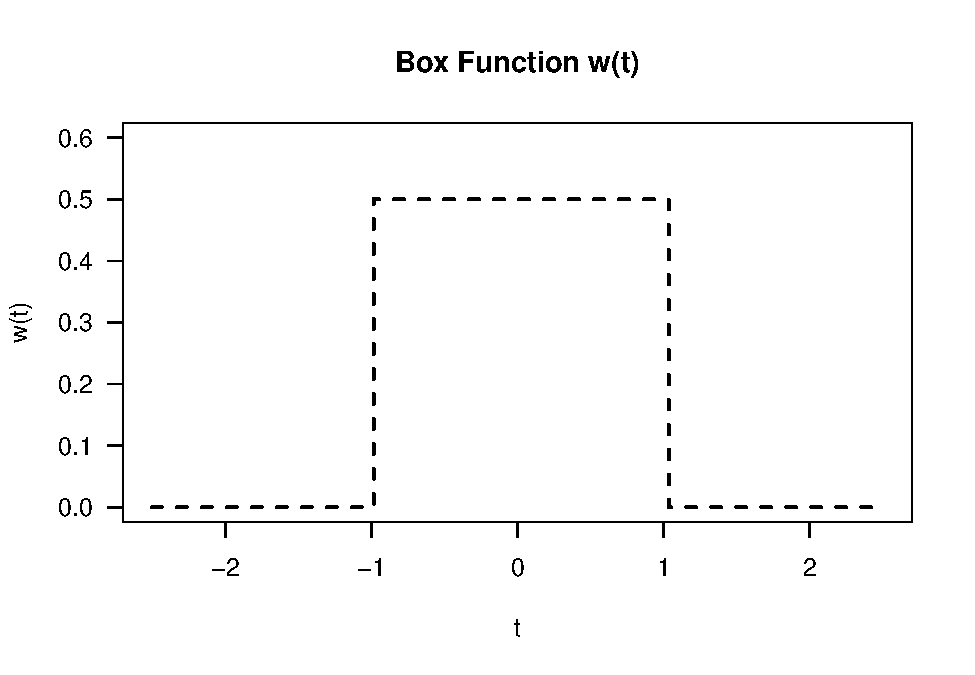
\includegraphics{08-densityestimation_files/figure-latex/unnamed-chunk-11-1.pdf}

\begin{itemize}
\item
  While the estimator \(\hat{f}_{h_{n}}^{B}\) does seem reasonable, it always
  results in density estimates which are not ``smooth.''
\item
  Most kernel density estimates are formed by replacing the box function \(w(t)\) with
  a smoother function.
\end{itemize}

\begin{center}\rule{0.5\linewidth}{\linethickness}\end{center}

\begin{itemize}
\item
  \textbf{Exercise 8.2}. Write an \textbf{R} function which computes the \(\hat{f}_{h_{n}}^{B}(x)\)
  at a collection of specified points.
\item
  \textbf{Exercise 8.3}. Suppose we have observations \((X_{1}, X_{2}, X_{3}, X_{4}) = (-1, 0, 1/2, 1)\).
  Assuming \(h_{n} = 1/2\), plot \(w(\tfrac{X_{i} - x}{h_{n}})/nh_{n}\) for \(i = 1, \ldots, 4\) and plot the box
  density estimate \(\hat{f}_{h_{n}}^{B}(x)\).
\item
  \textbf{Exercise 8.4}. Suppose we have i.i.d. observations \(X_{1}, \ldots, X_{n} \sim F\) where
  the cdf \(F\) is assumed to be continuous. What is \(\textrm{Var}\{ \hat{f}_{h_{n}}^{B}(x) \}\)?
\end{itemize}

\begin{center}\rule{0.5\linewidth}{\linethickness}\end{center}

\hypertarget{kernel-density-estimation}{%
\section{Kernel Density Estimation}\label{kernel-density-estimation}}

\hypertarget{definition-6}{%
\subsection{Definition}\label{definition-6}}

\begin{itemize}
\item
  Kernel density estimates are a generalization of the box-type density estimate \(\hat{f}_{h_{n}}^{B}(x)\).
\item
  With kernel density estimation, we replace the ``box function'' in \eqref{eq:box-density}
  with a function \(K(\cdot)\) which is much smoother.
\item
  The function \(K(\cdot)\) will also give higher weight to observations which are closer to \(x\)
  than those that are further away from \(x\).
\end{itemize}

\begin{center}\rule{0.5\linewidth}{\linethickness}\end{center}

\begin{itemize}
\item
  A kernel density estimator \(\hat{f}_{h_{n}}(x)\) is defined as
  \begin{equation}
  \hat{f}_{h_{n}}(x) = \frac{1}{nh_{n}} \sum_{i=1}^{n} K\Big( \frac{x - X_{i}}{h_{n}} \Big) 
  \label{eq:kernel-density-formula}
  \end{equation}
\item
  The function \(K( \cdot )\) is referred to as the \textbf{kernel function}.
\item
  The scalar term \(h_{n} > 0\) is called the \textbf{bandwidth}.
\item
  The value of the bandwidth \(h_{n}\) largely determines how ``bumpy'' the density estimate
  will appear.
\item
  The appearance and the statistical performance of \(\hat{f}_{h_{n}}(x)\) depend much more on the value of \(h_{n}\) than
  the choice of kernel function.
\end{itemize}

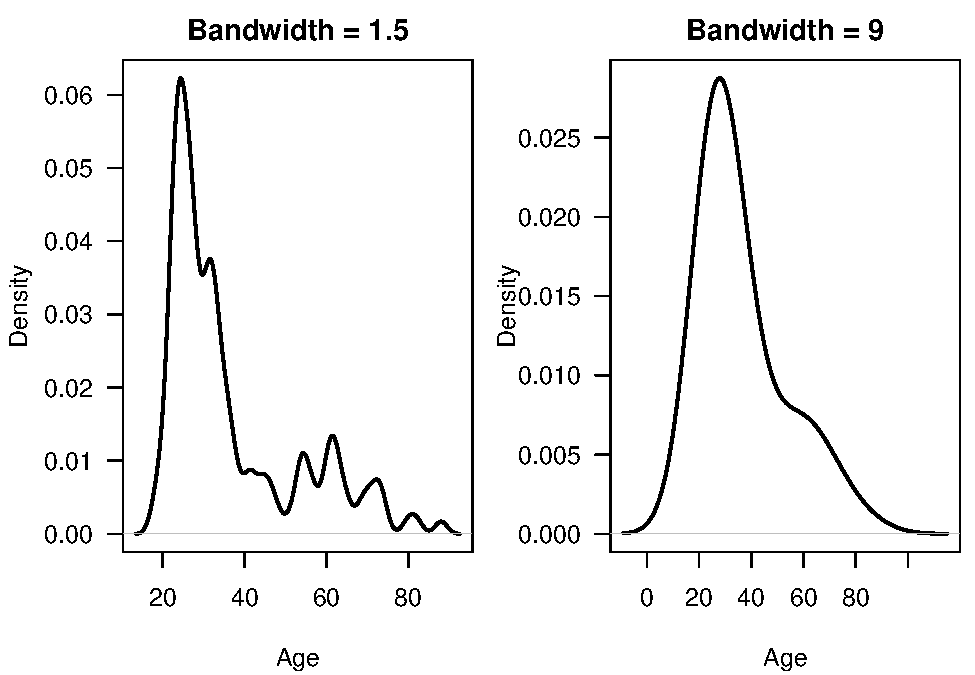
\includegraphics{08-densityestimation_files/figure-latex/unnamed-chunk-12-1.pdf}

\begin{center}\rule{0.5\linewidth}{\linethickness}\end{center}

\begin{itemize}
\item
  Kernel functions are usually chosen so that
  \begin{equation}
  K(t) \geq  0 \quad \textrm{ for all } t \nonumber 
  \end{equation}
  and that they also satisfy the following properties:
  \begin{eqnarray}
  K(t) = K(-t) \qquad 
  \int_{-\infty}^{\infty} K(t) dt = 1  \nonumber 
  \qquad 
  \int_{-\infty}^{\infty} K^{2}(t) dt  < \infty
  \nonumber
  \end{eqnarray}
\item
  You can think of \(K(u)\) as a probability density function
  which is symmetric around \(0\).
\item
  Some of the most common choices of kernel functions include
  \begin{eqnarray}
  \textrm{Gaussian} :&& \quad  K(u) = \exp(-u^{2}/2)/\sqrt{2\pi} \nonumber \\
  \textrm{Epanechnikov} :&& \quad  K(u) = \tfrac{3}{4\sqrt{5}}(1 - \tfrac{1}{5} u^{2}) I(|u| < \sqrt{5}) \nonumber \\
  \textrm{biweight} :&& \quad  K(u) = \tfrac{15}{16\sqrt{7}}(1 - \tfrac{1}{7} u^{2})^{2} I(|u| < \sqrt{7}) \nonumber \\
  \end{eqnarray}
\end{itemize}

\includegraphics{08-densityestimation_files/figure-latex/unnamed-chunk-13-1.pdf}

\begin{itemize}
\item
  When plotting \(\frac{1}{n h_{n}}K\big( \tfrac{x - X_{i}}{h_{n}} \big)\) as a function of \(x\), it should
  look like a ``small hill'' centered around \(X_{i}\).
\item
  As \(h_{n}\) decreases, \(\frac{1}{n h_{n}}K\big( \tfrac{x - X_{i}}{h_{n}} \big)\)
  becomes more strongly concentrated around \(X_{i}\) and has a higher peak.
\item
  The kernel density estimate \(\hat{f}_{h_{n}}(x)\) is a sum of all these ``small hills''.
\end{itemize}

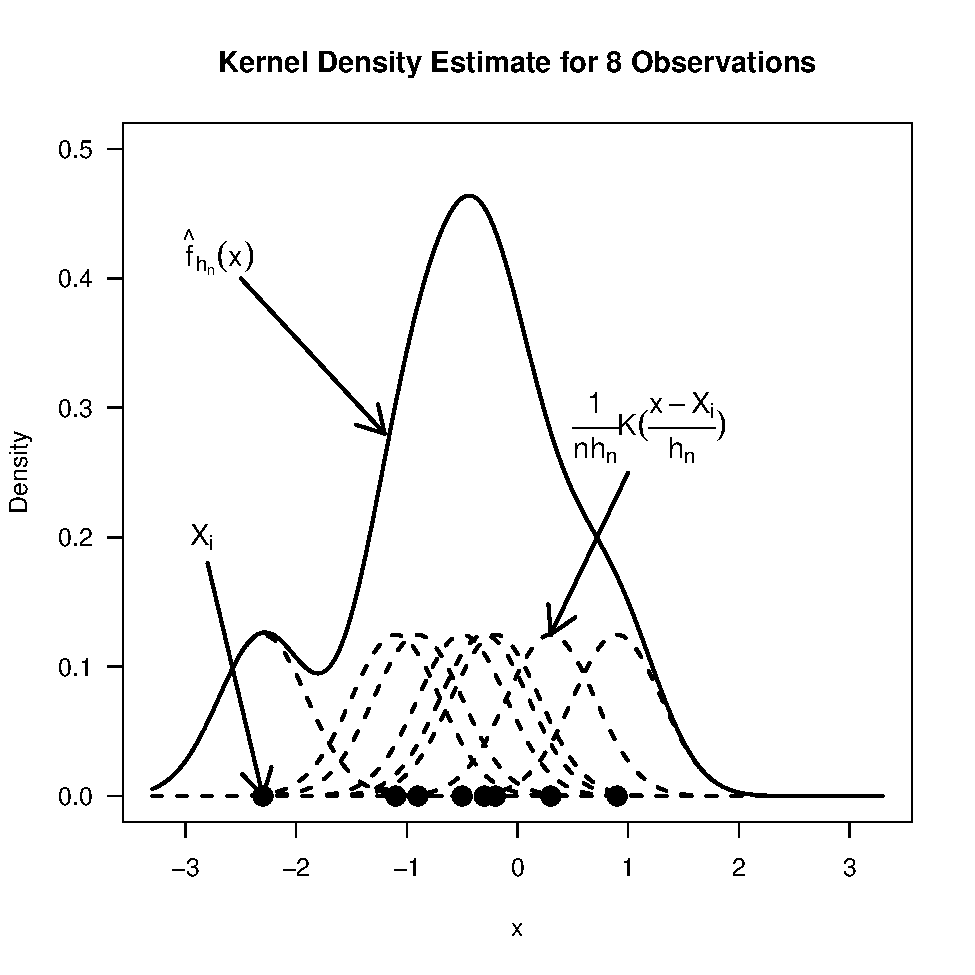
\includegraphics{08-densityestimation_files/figure-latex/unnamed-chunk-14-1.pdf}

\begin{center}\rule{0.5\linewidth}{\linethickness}\end{center}

\begin{itemize}
\item
  The nice thing about \eqref{eq:kernel-density-formula} is that it guarantees that \(\hat{f}_{h_{n}}(x)\) is a probability
  density function
  \begin{eqnarray}
  \int_{-\infty}^{\infty} \hat{f}_{h_{n}}(x) dx 
  &=& \int_{-\infty}^{\infty} \frac{1}{nh_{n}} \sum_{i=1}^{n} K\Big( \frac{x - X_{i}}{h_{n}} \Big)  dx  \nonumber \\
  &=&  \frac{1}{n} \sum_{i=1}^{n} \int_{-\infty}^{\infty} \frac{1}{h_{n}} K\Big( \frac{x - X_{i}}{h_{n}} \Big) dx  \nonumber \\
  &=& 1 \nonumber
  \end{eqnarray}
\item
  Also, formula \eqref{eq:kernel-density-formula} guarantees that \(\hat{f}_{h_{n}}(x)\) inherits the smoothness properties
  of \(K(u)\)
  \begin{equation}
  \hat{f}_{h_{n}}'(x) = \frac{1}{n} \sum_{i=1}^{n} \frac{1}{h_{n}^{2}} K'\Big( \frac{x - X_{i}}{h_{n}} \Big)  \nonumber
  \end{equation}
\end{itemize}

\hypertarget{bias-variance-and-amise-of-kernel-density-estimates}{%
\subsection{Bias, Variance, and AMISE of Kernel Density Estimates}\label{bias-variance-and-amise-of-kernel-density-estimates}}

\begin{itemize}
\tightlist
\item
  As with the bin width in histogram estimation, the bias/variance tradeoff
  drives the best choice of the bandwidth \(h_{n}\) in kernel density estimation.
\end{itemize}

\begin{center}\rule{0.5\linewidth}{\linethickness}\end{center}

\textbf{Approximate Bias}

\begin{itemize}
\item
  The exact expectation of a kernel density estimate \(\hat{f}_{h_{n}}(x)\) is
  \begin{eqnarray}
  E\{ \hat{f}_{h_{n}}(x) \}
  &=& \frac{1}{nh_{n}} \sum_{i=1}^{n} E\Big\{ K\Big( \frac{x - X_{i}}{h_{n}} \Big) \Big\} \nonumber \\
  &=& \frac{1}{h_{n}} E\Big\{ K\Big( \frac{x - X_{1}}{h_{n}} \Big) \Big\} \nonumber \\
  &=& \frac{1}{h_{n}} \int_{-\infty}^{\infty} K\Big( \frac{x - t}{h_{n}} \Big) f(t) dt \nonumber \\
  &=&  \int_{-\infty}^{\infty} K( u ) f(x - uh_{n}) du \nonumber 
  \end{eqnarray}
  Above, we used the substitution \(u = (x - t)/h_{n}\).
\item
  Thus, the exact bias of \(\hat{f}_{h_{n}}(x)\) is
  \begin{eqnarray}
  \textrm{Bias}\{ \hat{f}_{h_{n}}(x) \}
  &=& \int_{-\infty}^{\infty} K( u ) f(x - uh_{n}) du - f(x)  \nonumber \\
  &=& \int_{-\infty}^{\infty} K( u ) \{ f(x - uh_{n}) - f(x) \} du 
  \label{eq:exact-density-bias}
  \end{eqnarray}
\item
  The expression for bias shown in \eqref{eq:exact-density-bias} will only
  have a closed form for special choices of \(K(\cdot)\) and \(f( \cdot )\).
\item
  Nevertheless, we can get a reasonable approximation of this bias for small \(h_{n}\).
\item
  To approximate the bias for small \(h_{n}\), we can use the following Taylor series approximation
  \begin{equation}
  f(x - uh_{n}) - f(x) \approx -uh_{n}f'(x) + \frac{u^{2}h_{n}^{2}}{2} f''(x) \nonumber 
  \end{equation}
  Plugging this approximation into our expression for the bias in \eqref{eq:exact-density-bias} gives:
  \begin{eqnarray}
  \textrm{Bias}\{ \hat{f}_{h_{n}}(x) \}
  &\approx&  -h_{n}f'(x) \int_{-\infty}^{\infty} u K( u )  du + \frac{h_{n}^{2}f''(x)}{2} \int_{-\infty}^{\infty} u^{2} K( u ) du  \nonumber \\
  &=& \frac{h_{n}^{2}f''(x)}{2} \int_{-\infty}^{\infty} u^{2} K( u ) du \nonumber \\
  &=& \frac{h_{n}^{2}f''(x)\mu_{2}(K)}{2} \qquad \textrm{ where } \mu_{2}(K) = \int_{-\infty}^{\infty} u^{2} K( u ) du \nonumber \\
  &=& \textrm{ABias}\{ \hat{f}_{h_{n}}(x) \} 
  \label{eq:asymp-bias-density}
  \end{eqnarray}
  Here, \(\textrm{ABias}\{ \hat{f}_{h_{n}}(x) \}\) stands for the approximate bias.
\item
  Formula \eqref{eq:asymp-bias-density} shows the direct dependence of the magnitude of bias on
  the value of the bandwidth.
\item
  Formula \eqref{eq:asymp-bias-density} also shows the effect of the curvature \(f''(x)\)
  of the density on the magnitude of bias.
\end{itemize}

\begin{center}\rule{0.5\linewidth}{\linethickness}\end{center}

\textbf{Approximate Variance}

\begin{itemize}
\item
  The exact variance of a kernel density estimate \(\hat{f}_{h_{n}}(x)\) is
  \begin{eqnarray}
  \textrm{Var}\{ \hat{f}_{h_{n}}(x) \}
  &=& \frac{1}{n^{2}h_{n}^{2}} \sum_{i=1}^{n} \textrm{Var}\Big\{  K\Big( \frac{x - X_{i}}{ h_{n} } \Big) \Big\} \nonumber \\
  &=& \frac{1}{nh_{n}^{2}} \textrm{Var}\Big\{  K\Big( \frac{x - X_{1}}{ h_{n} } \Big) \Big\} \nonumber \\
  &=& \frac{1}{n h_{n}^{2} }\int_{-\infty}^{\infty} K^{2}\Big( \frac{x - t}{h_{n}} \Big) f(t) dt - \frac{1}{n}\Big[ \frac{1}{h_{n}}E\Big\{  K\Big( \frac{x - X_{1}}{ h_{n} } \Big) \Big\} \Big]^{2}  \nonumber \\
  &=& \frac{1}{n h_{n} }\int_{-\infty}^{\infty} K^{2}(u) f(x - uh_{n}) du - \frac{1}{n}\Big[ \textrm{Bias}\{ \hat{f}_{h_{n}}(x) \} + f(x) \Big]^{2} \nonumber
  \end{eqnarray}
\item
  We will ignore the last term because it is of order \(1/n\). Then, if we use the Taylor series approximation
  \(f(x - uh_{n}) = f(x) - uh_{n}f'(x) + ...\), we have:
  \begin{eqnarray}
  \textrm{Var}\{ \hat{f}_{h_{n}}(x) \}
  &\approx& \frac{f(x)}{n h_{n} }\int_{-\infty}^{\infty} K^{2}(u) du - \frac{f'(x)}{n}\int_{-\infty}^{\infty} u K^{2}(u) du  +  ... \nonumber \\
  &\approx& \frac{f(x)\kappa_{2}(K) }{n h_{n} } \quad \textrm{ where } \kappa_{2}(K) = \int_{-\infty}^{\infty} K^{2}( u ) du \nonumber \\
  &=& \textrm{AVar}\{ \hat{f}_{h_{n}}(x) \}  \nonumber
  \end{eqnarray}
\end{itemize}

\begin{center}\rule{0.5\linewidth}{\linethickness}\end{center}

\textbf{Approximate Mean Integrated Squared Error (AMISE)}

\begin{itemize}
\item
  Using our approximations for the bias and variance, we can get an approximate expression
  for the mean-squared error of \(\hat{f}_{h_{n}}(x)\) at the point \(x\)
  \begin{eqnarray}
  \textrm{MSE}\{ \hat{f}_{h_{n}}(x) \} 
  &\approx& 
  \textrm{AVar}\{ \hat{f}_{h_{n}}(x) \} + \Big( \textrm{ABias}\{ \hat{f}_{h_{n}}(x) \} \Big)^{2} \nonumber \\
  &=& \frac{f(x)\kappa_{2}(K) }{n h_{n} } + \frac{h_{n}^{4}[f''(x)]^{2}\mu_{2}^{2}(K)}{4} 
  \label{eq:asymp-mse-density}
  \end{eqnarray}
\item
  Notice that if we want the MSE to go to \(0\) as \(n \longrightarrow \infty\), we need the
  following two things to happen:

  \begin{itemize}
  \tightlist
  \item
    \(h_{n} \longrightarrow 0\) as \(n \longrightarrow \infty\)
  \item
    \(n h_{n} \longrightarrow \infty\) as \(n \longrightarrow \infty\)
  \end{itemize}
\end{itemize}

\begin{center}\rule{0.5\linewidth}{\linethickness}\end{center}

\begin{itemize}
\tightlist
\item
  The approximate mean integrated squared error (AMISE) is obtained by integrating
  the approximation \eqref{eq:asymp-mse-density} for MSE across \(x\)
  \begin{eqnarray}
  \textrm{AMISE}\{ \hat{f}_{h_{n}} \} &=& \frac{\kappa_{2}(K) }{n h_{n} }\int_{-\infty}^{\infty} f(x) dx + \frac{h_{n}^{4}\mu_{2}^{2}(K)}{4} \int_{-\infty}^{\infty} [f''(x)]^{2} dx \nonumber \\
  &=& \frac{\kappa_{2}(K) }{n h_{n} } + \frac{h_{n}^{4}\mu_{2}^{2}(K)}{4} \int_{-\infty}^{\infty} [f''(x)]^{2} dx
  \label{eq:amise-density}
  \end{eqnarray}
\end{itemize}

\hypertarget{bandwidth-selection-with-the-normal-reference-rule-and-silvermans-rule-of-thumb}{%
\subsection{Bandwidth Selection with the Normal Reference Rule and Silverman's ``Rule of Thumb''}\label{bandwidth-selection-with-the-normal-reference-rule-and-silvermans-rule-of-thumb}}

\begin{itemize}
\item
  If we differentiate the formula for AMISE given in \eqref{eq:amise-density} with respect to \(h_{n}\) and set it to zero,
  we get the following equation for \(h_{n}^{opt}\) which would be the bandwidth minimizing \(\textrm{AMISE}\{ \hat{f}_{h_{n}} \}\):
  \begin{equation}
  0 = \frac{-\kappa_{2}(K) }{n (h_{n}^{opt})^{2} } + (h_{n}^{opt})^{3}\mu_{2}^{2}(K) \int_{-\infty}^{\infty} [f''(x)]^{2} dx \nonumber
  \end{equation}
\item
  The solution of the above equation gives the optimal bandwidth:
  \begin{equation}
  h_{n}^{opt} = n^{-1/5} \Big( \int_{-\infty}^{\infty} [f''(x)]^{2} dx \Big)^{-1/5}\kappa_{2}(K)^{1/5} \mu_{2}(K)^{-2/5} \nonumber
  \end{equation}
\item
  For the case of a Gaussian kernel,
  \begin{eqnarray}
  \kappa_{2}(K) &=& \frac{1}{2\pi}\int_{-\infty}^{\infty} e^{-u^{2}} du = \frac{1}{2\sqrt{\pi}}\int_{-\infty}^{\infty} \frac{\sqrt{2}}{\sqrt{2\pi}} e^{-u^{2}} du = \frac{1}{2\sqrt{\pi}} \nonumber \\
  \mu_{2}(K) &=& \frac{1}{\sqrt{2\pi}}\int_{-\infty}^{\infty} u^{2}e^{-u^{2}/2} du = 1
  \end{eqnarray}
  so that, in the case of a Gaussian kernel, the optimal bandwidth is given by
  \begin{equation}
  h_{n}^{opt} = n^{-1/5} (2\sqrt{\pi})^{-1/5} \Big( \int_{-\infty}^{\infty} [f''(x)]^{2} dx \Big)^{-1/5}
  \end{equation}
\item
  The optimal bandwidth \(h_{n}^{opt}\) for a kernel density estimate depends on the unknown quantity
  \begin{equation}
  \int_{-\infty}^{\infty} [f''(x)]^{2} dx  \nonumber
  \end{equation}
\end{itemize}

\begin{center}\rule{0.5\linewidth}{\linethickness}\end{center}

\begin{itemize}
\item
  Similar to the Scott and FD rules for choosing the bin width of histogram, one way of setting the bandwidth \(h_{n}\)
  of a kernel density estimate is to use the value of \(\int_{-\infty}^{\infty} [f''(x)]^{2} dx\) when it is assumed that
  \(f(x)\) is the density of a \(\textrm{Normal}(0, \sigma^{2})\) random variable.
\item
  If \(f(x) = \textrm{Normal}(0, \sigma^{2})\), then
  \begin{equation}
  \int_{-\infty}^{\infty} [f''(x)]^{2} dx = \frac{3}{8\sqrt{\pi}\sigma^{5}} \nonumber 
  \end{equation}
\item
  If we use this assumption about \(f''(x)\) for the case of a Gaussian kernel, the formula for the optimal bandwidth becomes
  bandwidth is
  \begin{equation}
  h_{n}^{opt} = n^{-1/5}(2\sqrt{\pi})^{-1/5}\Big( \frac{3}{8\sqrt{\pi}\sigma^{5}} \Big)^{-1/5}
  = \sigma n^{-1/5} \sigma \Big( \frac{4}{3} \Big)^{1/5}
  \approx 1.06 \sigma n^{-1/5}
  \end{equation}
\end{itemize}

\begin{center}\rule{0.5\linewidth}{\linethickness}\end{center}

\begin{itemize}
\item
  The rule \(h_{n}^{opt} = 1.06 \sigma n^{-1/5}\) works pretty well if the true density has a roughly Gaussian shape. For example,
  unimodal, non-heavy tails, not too strong skewness, etc.
\item
  The \textbf{Normal reference rule} for the bandwidth is
  \begin{equation}
  h_{n}^{NR} = 1.06 \tilde{\sigma} n^{-1/5}  \nonumber
  \end{equation}
\item
  Here, \(\tilde{\sigma}\) is usually either \(\tilde{\sigma} = \hat{\sigma}\) or \(\tilde{\sigma} = s\).
\item
  \(h_{n} = 1.06 \hat{\sigma} n^{-1/5}\) is typically too large if \(f(x)\) is multimodal or
  if \(f(x)\) has substantial skewness.
\item
  This oversmoothing effect of \(h_{n} = 1.06 \hat{\sigma} n^{-1/5}\) can be reduced somewhat by replacing \(\hat{\sigma}\) with
  \begin{equation}
  s = \min\Big\{ \hat{\sigma}, \frac{IQR}{1.34} \Big\} \nonumber 
  \end{equation}
\item
  For multimodal distributions, we typically have \(\hat{\sigma} \leq IQR/1.34\) while for strongly skewed
  distributions such as the log-normal distribution we typically have \(\hat{\sigma} \geq IQR/1.34\).
\item
  For these reasons, \(\tilde{\sigma} = s\) is often suggested when using the Normal reference rule.
\end{itemize}

\begin{center}\rule{0.5\linewidth}{\linethickness}\end{center}

\begin{itemize}
\item
  Silverman's ``rule-of-thumb'' for the bandwidth is
  \begin{equation}
  h_{n}^{SR} = 0.9 s n^{-1/5}  \nonumber
  \end{equation}
  (see Chapter 3 of \citet{silverman2018}).
\item
  This rule is just an adjustment for the fact that \(1.06 s n^{-1/5}\) is still
  too large for many skewed or multimodal distribution and using \(0.9\) instead of \(1.06\) reduces
  this problem.
\end{itemize}

\begin{center}\rule{0.5\linewidth}{\linethickness}\end{center}

\begin{itemize}
\item
  \textbf{Exercise 8.5} Assuming that \(f(x) = \tfrac{1}{\sqrt{2\pi}\sigma}e^{-x^{2}/2\sigma^{2}}\), show
  that
  \begin{equation}
  \int_{-\infty}^{\infty} [f''(x)]^{2} dx = \frac{3}{8\sqrt{\pi}\sigma^{5}} \nonumber
  \end{equation}
\item
  \textbf{Exercise 8.6} Suppose \(X_{1}, \ldots, X_{n} \sim N(0, \sigma^{2})\). Suppose that
  we have density estimate \(\hat{f}_{h_{n}}(x)\) that uses the Gaussian kernel.

  \begin{itemize}
  \tightlist
  \item
    Compute the exact values of \(E\{ \hat{f}_{h_{n}}(x) \}\) and \(\textrm{Var}\{ \hat{f}_{h_{n}}(x) \}\).
  \item
    Compute AMISE\(\{ \hat{f}_{h_{n}} \}\). Can you get an expression for the value of \(h_{n}\) which minimizes AMISE?
  \end{itemize}
\end{itemize}

\begin{center}\rule{0.5\linewidth}{\linethickness}\end{center}

\hypertarget{cross-validation-for-bandwidth-selection}{%
\section{Cross-Validation for Bandwidth Selection}\label{cross-validation-for-bandwidth-selection}}

\hypertarget{squared-error-cross-validation}{%
\subsection{Squared-Error Cross-Validation}\label{squared-error-cross-validation}}

\begin{itemize}
\item
  The usual goal in bandwidth selection is to choose the bandwidth
  which minimizes the mean integrated squared error (MISE)
  \begin{equation}
  \textrm{MISE}(h) = E\Big[ \int \{ \hat{f}_{h}(x) - f(x)   \}^{2} dx \Big]
  \end{equation}
  or some related criterion which also measures an expected discrepancy between \(\hat{f}_{h}(x)\) and \(f(x)\).
\item
  The MISE can be rewritten as
  \begin{equation}
  \textrm{MISE}(h) = E\Big[ \int \hat{f}_{h}^{2}(x) dx \Big]  - 2 \int E\Big[ \hat{f}_{h}(x) \Big] f(x) dx + \int f^{2}(x) dx
  \label{eq:mise-decomposition}
  \end{equation}
\item
  If the goal is to minimize \(\textrm{MISE}(h)\), we can ignore the last term since it does not depend on \(h\).
\end{itemize}

\begin{center}\rule{0.5\linewidth}{\linethickness}\end{center}

\begin{itemize}
\item
  Our goal will be find a bandwidth that minimizes an estimate of \(\textrm{MISE}(h)\) (an estimate which ignores the last term in \eqref{eq:mise-decomposition}),
  and this estimate will use a technique called leave-one-out \textbf{cross-validation}.
\item
  Regarding the first term in \eqref{eq:mise-decomposition}, we can just estimate this expectation with
  \begin{equation}
  \int \hat{f}_{h}^{2}(x) dx  \nonumber 
  \end{equation}
\item
  The second term in \eqref{eq:mise-decomposition} is trickier because it has \(f(x)\) in it.
\item
  We can simplify this term though
  \begin{equation}
  \int E\Big[ \hat{f}_{h}(x) \Big] f(x) dx = E\Bigg[ \frac{1}{h} K\Big( \frac{X_{1} - X_{2}}{h} \Big)  \Bigg] \nonumber 
  \end{equation}
  (why is this true?)
\end{itemize}

\begin{center}\rule{0.5\linewidth}{\linethickness}\end{center}

\begin{itemize}
\item
  We can construct an estimate of \eqref{eq:mise-decomposition} by first defining the
  following ``leave-one-out'' estimate
  \begin{equation}
  \hat{f}_{h, -i}(x) = \frac{1}{(n-1)h}\sum_{j \neq i}  K\Big( \frac{x - X_{j}}{h} \Big) 
  \end{equation}
\item
  In other words, \(\hat{f}_{h, -i}(x)\) is a density estimate constructed from using
  bandwidth \(h\) and all the data except for the \(i^{th}\) observation.
\item
  Then, we are going use the following quantity to estimate \(\int E[ \hat{f}_{h}(x) ] f(x) dx\)
  \begin{equation}
  \frac{1}{n} \sum_{i=1}^{n} \hat{f}_{h, -i}( X_{i} ) 
  = \frac{1}{n(n-1)} \sum_{i=1}^{n} \sum_{j \neq i} \frac{1}{h}K\Big( \frac{X_{i} - X_{j}}{ h } \Big) \nonumber 
  \end{equation}
\item
  The term \(\frac{1}{n} \sum_{i=1}^{n} \hat{f}_{h, -i}( X_{i} )\) is referred to as a leave-one-out cross-validation
  estimate.
\item
  The expectation of this quantity is
  \begin{eqnarray}
  E\Big\{ \frac{1}{n} \sum_{i=1}^{n} \hat{f}_{h, -i}( X_{i} )  \Big\}
  &=& \frac{1}{n(n-1)}\sum_{i=1}^{n} \sum_{j \neq i} E\Big\{ \frac{1}{h}  K\Big( \frac{X_{i} - X_{j}}{ h } \Big)  \Big\}  \nonumber \\
  &=& E\Big\{ \frac{1}{h}  K\Big( \frac{X_{1} - X_{2}}{ h } \Big)  \Big\} \nonumber
  \end{eqnarray}
\end{itemize}

\begin{center}\rule{0.5\linewidth}{\linethickness}\end{center}

\begin{itemize}
\item
  The leave-one-out \textbf{cross-validation estimate of the MISE} (ignoring the irrelevant \(\int f^{2}(x) dx\)) is
  \begin{equation}
  \hat{J}_{MISE}(h) = \int \hat{f}_{h}^{2}(x) dx - \frac{2}{n} \sum_{i=1}^{n} \hat{f}_{h, -i}( X_{i} )  \nonumber
  \end{equation}
\item
  The integrated squared error cross-validation choice of the bandwidth \(h_{n,cv}\) is the value of \(h > 0\) which minimizes \(\hat{J}_{MISE}(h)\)
  \begin{equation}
  h_{n,cv} = \arg\min_{h > 0} \hat{J}_{MISE}(h) \nonumber
  \end{equation}
\end{itemize}

\hypertarget{computing-the-cross-validation-bandwidth}{%
\subsection{Computing the Cross-validation Bandwidth}\label{computing-the-cross-validation-bandwidth}}

\begin{itemize}
\item
  \textbf{R} does have built-in capabilities for finding the bandwidth through cross-validation, but
  let's do an example ourselves to see how the process works.
\item
  First, we can build a function called \texttt{J\_mise} that has input and output:

  \begin{itemize}
  \tightlist
  \item
    Input: a value of the bandwidth \(h\) and a vector of data
  \item
    Output: the value of \(\hat{J}_{MISE}(h)\)
  \end{itemize}
\end{itemize}

\begin{Shaded}
\begin{Highlighting}[]
\NormalTok{J_mise <-}\StringTok{ }\ControlFlowTok{function}\NormalTok{(h, x) \{}
\NormalTok{    n <-}\StringTok{ }\KeywordTok{length}\NormalTok{(x)}
\NormalTok{    loo.val <-}\StringTok{ }\KeywordTok{rep}\NormalTok{(}\DecValTok{0}\NormalTok{, n)}
    \ControlFlowTok{for}\NormalTok{(k }\ControlFlowTok{in} \DecValTok{1}\OperatorTok{:}\NormalTok{n) \{}
        \CommentTok{## compute the leave-one-out density estimate}
        \CommentTok{## only focus on density on interval (18, 90)}
\NormalTok{        loo.fhat <-}\StringTok{ }\KeywordTok{density}\NormalTok{(x[}\OperatorTok{-}\NormalTok{k], }\DataTypeTok{bw=}\NormalTok{h, }\DataTypeTok{from=}\DecValTok{18}\NormalTok{, }\DataTypeTok{to=}\DecValTok{90}\NormalTok{)}
\NormalTok{        loo.fhat.fn <-}\StringTok{ }\KeywordTok{approxfun}\NormalTok{(loo.fhat}\OperatorTok{$}\NormalTok{x, loo.fhat}\OperatorTok{$}\NormalTok{y)}
\NormalTok{        loo.val[k] <-}\StringTok{ }\KeywordTok{loo.fhat.fn}\NormalTok{(x[k])}
\NormalTok{    \}}
\NormalTok{    fhat <-}\StringTok{ }\KeywordTok{density}\NormalTok{(x, }\DataTypeTok{bw=}\NormalTok{h, }\DataTypeTok{from=}\DecValTok{18}\NormalTok{, }\DataTypeTok{to=}\DecValTok{90}\NormalTok{)}
\NormalTok{    fhat.sq.fn <-}\StringTok{ }\KeywordTok{approxfun}\NormalTok{(fhat}\OperatorTok{$}\NormalTok{x, fhat}\OperatorTok{$}\NormalTok{y}\OperatorTok{^}\DecValTok{2}\NormalTok{)}
    
\NormalTok{    ans <-}\StringTok{ }\KeywordTok{integrate}\NormalTok{(fhat.sq.fn, }\DataTypeTok{lower=}\DecValTok{18}\NormalTok{, }\DataTypeTok{upper=}\DecValTok{90}\NormalTok{)}\OperatorTok{$}\NormalTok{value }\OperatorTok{-}\StringTok{ }\DecValTok{2}\OperatorTok{*}\KeywordTok{mean}\NormalTok{(loo.val)}
    \KeywordTok{return}\NormalTok{(ans)}
\NormalTok{\}}
\end{Highlighting}
\end{Shaded}

\begin{itemize}
\item
  Now, we want to use our \textbf{R} function to compute \(\hat{J}(h_{j})\) over
  a grid of bandwidth values
  \begin{equation}
  h_{min} \leq h_{1} < ... < h_{q} \leq h_{max} \nonumber
  \end{equation}
\item
  The smallest and largest possible bandwidths \(h_{min}\) and \(h_{max}\) can be chosen
  by looking at plots of the density for different bandwidths.
\item
  \(h_{min}\) should correspond
  to a density estimate which is very nonsmooth while \(h_{max}\) should correspond to
  a density which is oversmoothed.
\item
  For the ages from the kidney data, \(h_{min} = 1/2\) and \(h_{max} = 5\) seem like reasonable choices.
\item
  Let us compute \(\hat{J}(h)\) for a grid of \(100\) bandwidths between \(1/2\) and \(5\):
\end{itemize}

\begin{Shaded}
\begin{Highlighting}[]
\NormalTok{h.grid <-}\StringTok{ }\KeywordTok{seq}\NormalTok{(}\DecValTok{1}\OperatorTok{/}\DecValTok{2}\NormalTok{, }\DecValTok{5}\NormalTok{, }\DataTypeTok{length.out=}\DecValTok{100}\NormalTok{)}
\NormalTok{CV.est <-}\StringTok{ }\KeywordTok{rep}\NormalTok{(}\DecValTok{0}\NormalTok{, }\DecValTok{100}\NormalTok{)}
\ControlFlowTok{for}\NormalTok{(j }\ControlFlowTok{in} \DecValTok{1}\OperatorTok{:}\DecValTok{100}\NormalTok{) \{}
\NormalTok{   CV.est[j] <-}\StringTok{ }\KeywordTok{J_mise}\NormalTok{(}\DataTypeTok{h=}\NormalTok{h.grid[j], }\DataTypeTok{x=}\NormalTok{kidney}\OperatorTok{$}\NormalTok{age)}
\NormalTok{\}}
\end{Highlighting}
\end{Shaded}

\begin{itemize}
\tightlist
\item
  Now, if we plot \(\hat{J}(h)\) vs. \(h\), we can see what the best value of the bandwidth is.
  From the graph, it appears that a bandwidth of roughly \(h = 1.8\) minimizes \(\hat{J}(h)\)
\end{itemize}

\begin{Shaded}
\begin{Highlighting}[]
\KeywordTok{plot}\NormalTok{(h.grid, CV.est, }\DataTypeTok{xlab=}\StringTok{"bandwidth"}\NormalTok{, }\DataTypeTok{ylab=}\StringTok{"J_mise(h)"}\NormalTok{, }
     \DataTypeTok{main =} \StringTok{"Cross-Validation Estimates for Age Data"}\NormalTok{)}
\end{Highlighting}
\end{Shaded}

\includegraphics{08-densityestimation_files/figure-latex/unnamed-chunk-17-1.pdf}

\begin{itemize}
\tightlist
\item
  The specific value of the bandwidth where \(\hat{J}(h_{j})\) reaches its minimum is:
\end{itemize}

\begin{Shaded}
\begin{Highlighting}[]
\NormalTok{h.grid[ }\KeywordTok{which.min}\NormalTok{(CV.est) ]}
\end{Highlighting}
\end{Shaded}

\begin{verbatim}
## [1] 1.772727
\end{verbatim}

\hypertarget{likelihood-cross-validation}{%
\subsection{Likelihood Cross-Validation}\label{likelihood-cross-validation}}

\begin{itemize}
\item
  An alternative criterion to use is the \textbf{Kullback-Leibler (KL) divergence}
  \begin{equation}
  \textrm{KL}(h) = \int \log \Big( \frac{ f(x) }{ \hat{f}_{h}(x) } \Big)  f(x) dx
  = -\int \log \{ \hat{f}_{h}(x) \}  f(x) dx + \int \log\{ f(x) \}f(x) dx
  \end{equation}
\item
  We only need to get an estimate of \(\int \log \{ \hat{f}_{h}(x) \} f(x) dx\)
  because \(\int \log\{ f(x) \}f(x) dx\) does not depend on \(h\).
\item
  We can use the same approach as we did for integrated squared error cross-validation
  to estimate \(\int \log \{ \hat{f}_{h}(x) \} f(x) dx\).
\item
  The leave-one-out \textbf{cross-validation estimate of the KL divergence} (ignoring the irrelevant \(\int \log\{ f(x) \}f(x) dx\) term) is
  \begin{equation}
  \hat{J}_{KL}(h) = -\frac{1}{n} \sum_{i=1}^{n} \log \{ \hat{f}_{h, -i}( X_{i} ) \}  \nonumber
  \end{equation}
\item
  Choosing the bandwidth which minimizes \(\hat{J}_{KL}(h)\) is often referred to as \textbf{likelihood cross-validation}.
\item
  An \textbf{R} function which can compute \(\hat{J}_{KL}(h)\) is given below:
\end{itemize}

\begin{Shaded}
\begin{Highlighting}[]
\NormalTok{J_KL <-}\StringTok{ }\ControlFlowTok{function}\NormalTok{(h, x) \{}
\NormalTok{  n <-}\StringTok{ }\KeywordTok{length}\NormalTok{(x)}
\NormalTok{  loo.val <-}\StringTok{ }\KeywordTok{rep}\NormalTok{(}\DecValTok{0}\NormalTok{, n)}
  \ControlFlowTok{for}\NormalTok{(k }\ControlFlowTok{in} \DecValTok{1}\OperatorTok{:}\NormalTok{n) \{}
    \CommentTok{## compute the leave-one-out density estimate}
    \CommentTok{## only focus on density on interval (18, 90)}
\NormalTok{    loo.fhat <-}\StringTok{ }\KeywordTok{density}\NormalTok{(x[}\OperatorTok{-}\NormalTok{k], }\DataTypeTok{bw=}\NormalTok{h, }\DataTypeTok{from=}\DecValTok{18}\NormalTok{, }\DataTypeTok{to=}\DecValTok{90}\NormalTok{)}
\NormalTok{    loo.fhat.fn <-}\StringTok{ }\KeywordTok{approxfun}\NormalTok{(loo.fhat}\OperatorTok{$}\NormalTok{x, loo.fhat}\OperatorTok{$}\NormalTok{y)}
\NormalTok{    loo.val[k] <-}\StringTok{ }\NormalTok{(}\OperatorTok{-}\DecValTok{1}\NormalTok{)}\OperatorTok{*}\KeywordTok{log}\NormalTok{(}\KeywordTok{loo.fhat.fn}\NormalTok{(x[k]))}
\NormalTok{  \}}
  \KeywordTok{return}\NormalTok{(}\KeywordTok{mean}\NormalTok{(loo.val))}
\NormalTok{\}}
\end{Highlighting}
\end{Shaded}

\begin{center}\rule{0.5\linewidth}{\linethickness}\end{center}

\begin{itemize}
\tightlist
\item
  \textbf{Exercise 8.7} Using the \textbf{age} variable from the kidney function data,
  find the best bandwidth using a Gaussian kernel and likelihood cross-validation.
\end{itemize}

\begin{center}\rule{0.5\linewidth}{\linethickness}\end{center}

\hypertarget{density-estimation-in-r}{%
\section{Density Estimation in R}\label{density-estimation-in-r}}

\begin{itemize}
\tightlist
\item
  In \textbf{R}, kernel density estimates are computed using the \texttt{density} function
\end{itemize}

\begin{Shaded}
\begin{Highlighting}[]
\KeywordTok{density}\NormalTok{(x, bw, kernel, n, ...)}
\end{Highlighting}
\end{Shaded}

\begin{itemize}
\item
  \textbf{x} - the vector containing the data
\item
  \textbf{bw} - the value of the bandwidth.

  \begin{itemize}
  \tightlist
  \item
    \texttt{bw\ =\ nrd0} gives the default bandwidth rule. This is Silverman's rule-of-thumb \(h_{n} = 0.9 s n^{-1/5}\)
  \item
    \texttt{bw\ =\ nrd} gives the bandwidth \(h_{n} = 1.06 \hat{\sigma} n^{-1/5}\)
  \item
    \texttt{bw\ =\ ucv} or \texttt{bw\ =\ bcv} find the bandwidth using cross-validation
  \end{itemize}
\item
  \textbf{kernel} - the choice of kernel function. The default kernel is the Gaussian kernel.
\item
  Be careful, some of the non-Gaussian kernels used in the \texttt{density} function are scaled differently than the definitions you might often see in textbooks or on-line resources.
\item
  \textbf{n} - the number of equally spaced points at which the density is to be estimated. The default is 512
\end{itemize}

\begin{center}\rule{0.5\linewidth}{\linethickness}\end{center}

\begin{itemize}
\tightlist
\item
  In this section, we will use the \texttt{galaxies} dataset in the \texttt{MASS} package.
  The first few observations of the \texttt{galaxies} dataset look like:
\end{itemize}

\begin{Shaded}
\begin{Highlighting}[]
\KeywordTok{library}\NormalTok{(MASS)}
\NormalTok{galaxies[}\DecValTok{1}\OperatorTok{:}\DecValTok{5}\NormalTok{]}
\end{Highlighting}
\end{Shaded}

\begin{verbatim}
## [1] 9172 9350 9483 9558 9775
\end{verbatim}

\begin{itemize}
\tightlist
\item
  Kernel density estimates can be computed in \textbf{R} using the \texttt{density} function
\end{itemize}

\begin{Shaded}
\begin{Highlighting}[]
\NormalTok{galax.dens <-}\StringTok{ }\KeywordTok{density}\NormalTok{(galaxies)}
\end{Highlighting}
\end{Shaded}

\begin{itemize}
\tightlist
\item
  You can display a density plot just by applying the \texttt{plot} function to our \texttt{galax.dens} object
\end{itemize}

\begin{Shaded}
\begin{Highlighting}[]
\KeywordTok{plot}\NormalTok{(galax.dens, }\DataTypeTok{main=}\StringTok{"Default Density Estimate for Galaxy Data"}\NormalTok{, }
     \DataTypeTok{xlab=}\StringTok{"velocity in km/sec"}\NormalTok{, }\DataTypeTok{ylab=}\StringTok{"Density"}\NormalTok{, }\DataTypeTok{lwd=}\DecValTok{2}\NormalTok{)}
\end{Highlighting}
\end{Shaded}

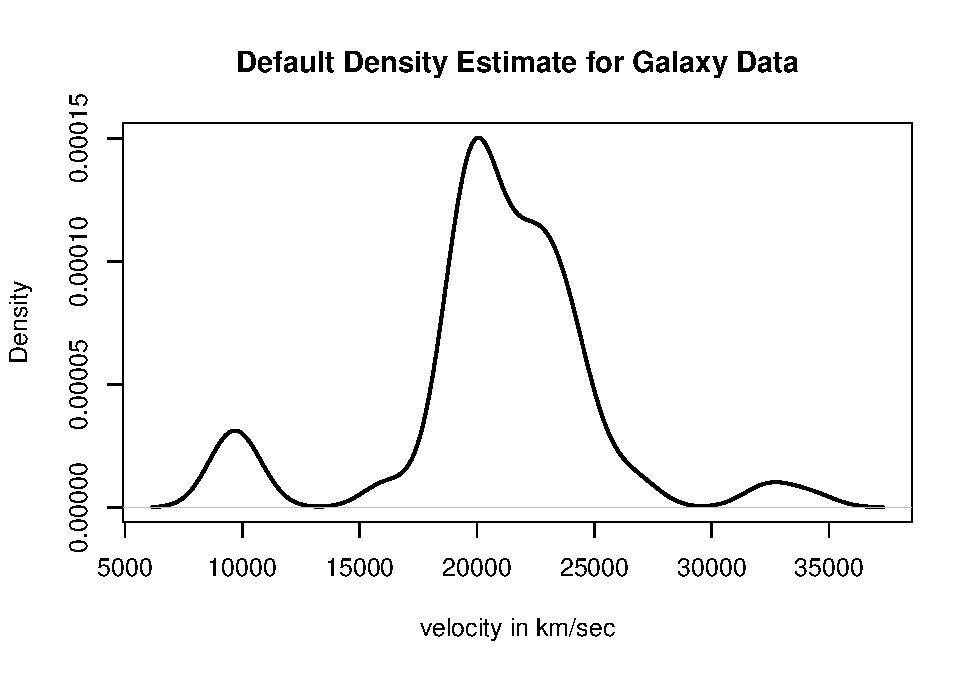
\includegraphics{08-densityestimation_files/figure-latex/unnamed-chunk-23-1.pdf}

\begin{center}\rule{0.5\linewidth}{\linethickness}\end{center}

\begin{itemize}
\tightlist
\item
  The density function returns vectors \texttt{x} and \texttt{y} as components

  \begin{itemize}
  \tightlist
  \item
    \texttt{x} - the vector of points at which the density was estimated
  \item
    \texttt{y} - the value of the estimated density at each of the \texttt{x} points
  \end{itemize}
\item
  So, just plotting the \texttt{(x,\ y)} should give you a plot of the density estimate
\end{itemize}

\begin{Shaded}
\begin{Highlighting}[]
\KeywordTok{plot}\NormalTok{(galax.dens}\OperatorTok{$}\NormalTok{x, galax.dens}\OperatorTok{$}\NormalTok{y, }\DataTypeTok{main=}\StringTok{"Default Density Estimate for Galaxy Data"}\NormalTok{, }
     \DataTypeTok{xlab=}\StringTok{"velocity in km/sec"}\NormalTok{, }\DataTypeTok{ylab=}\StringTok{"Density"}\NormalTok{, }\DataTypeTok{lwd=}\DecValTok{2}\NormalTok{)}
\end{Highlighting}
\end{Shaded}

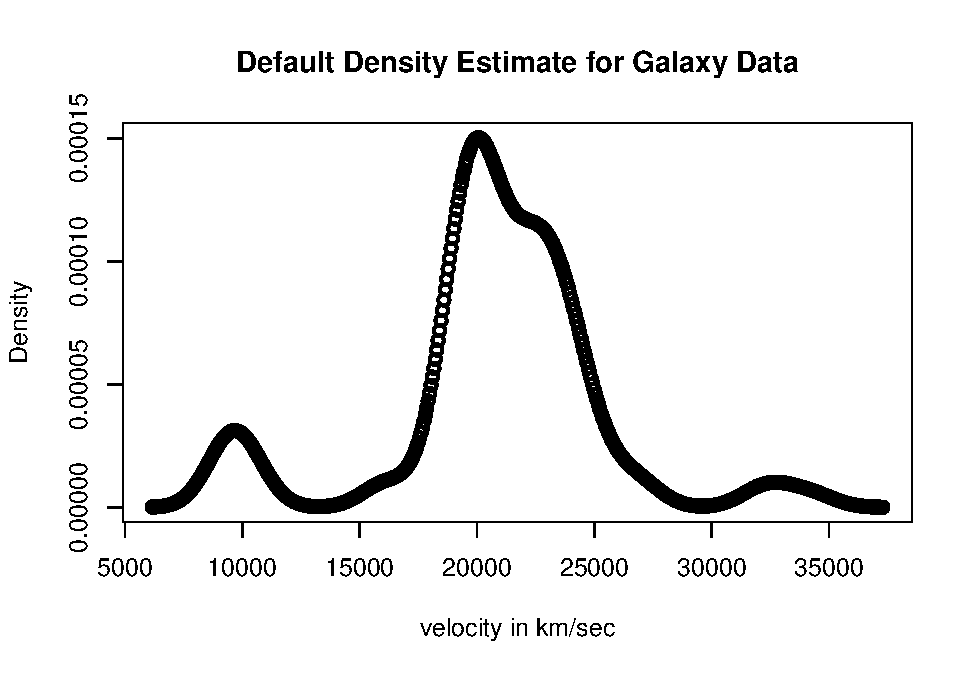
\includegraphics{08-densityestimation_files/figure-latex/unnamed-chunk-24-1.pdf}

\begin{itemize}
\tightlist
\item
  The default in \textbf{R} is to estimate the density at 512 points. Thus, \texttt{galax.dens\$x}
  and \texttt{galax.dens\$y} should have length 512.
\end{itemize}

\begin{center}\rule{0.5\linewidth}{\linethickness}\end{center}

\begin{itemize}
\tightlist
\item
  The \texttt{bw} component returned by the \texttt{density} function is the bandwidth used to estimate the density.
\end{itemize}

\begin{Shaded}
\begin{Highlighting}[]
\NormalTok{galax.dens}\OperatorTok{$}\NormalTok{bw}
\end{Highlighting}
\end{Shaded}

\begin{verbatim}
## [1] 1001.839
\end{verbatim}

\begin{itemize}
\item
  The default bandwidth selection rule in \textbf{R} is Silverman's rule-of-thumb \(h_{n}^{SR} = 0.9 s n^{-1/5}\).
\item
  We can check that this is true with the following code:
\end{itemize}

\begin{Shaded}
\begin{Highlighting}[]
\FloatTok{0.9}\OperatorTok{*}\KeywordTok{min}\NormalTok{(}\KeywordTok{sd}\NormalTok{(galaxies), }\KeywordTok{IQR}\NormalTok{(galaxies)}\OperatorTok{/}\FloatTok{1.34}\NormalTok{)}\OperatorTok{/}\NormalTok{(}\KeywordTok{length}\NormalTok{(galaxies)}\OperatorTok{^}\NormalTok{(}\DecValTok{1}\OperatorTok{/}\DecValTok{5}\NormalTok{))}
\end{Highlighting}
\end{Shaded}

\begin{verbatim}
## [1] 1001.839
\end{verbatim}

\begin{center}\rule{0.5\linewidth}{\linethickness}\end{center}

\begin{itemize}
\item
  The \textbf{R} function \texttt{approxfun} is useful if you want to compute the (approximate) value of the density
  estimate at a particular point. This approximation will be very close to the true value since
  the \texttt{density} function returns the value of the density over a dense grid of points.
\item
  \texttt{approxfun} just linearly interpolates between a set of x and y values.
\item
  Note that, as a default, \texttt{approxfun} returns NA values if you try to evaluate the function
  at points which are either less than the minimum x value or greater than maximum x value.
\item
  For example, suppose we want to know the value of the density estimate at the points \(18000\)
  and \(33000\). This could be done with the following code
\end{itemize}

\begin{Shaded}
\begin{Highlighting}[]
\NormalTok{galaxy.fn <-}\StringTok{ }\KeywordTok{approxfun}\NormalTok{(galax.dens}\OperatorTok{$}\NormalTok{x, galax.dens}\OperatorTok{$}\NormalTok{y)}

\KeywordTok{galaxy.fn}\NormalTok{(}\DecValTok{18000}\NormalTok{)}
\end{Highlighting}
\end{Shaded}

\begin{verbatim}
## [1] 4.73857e-05
\end{verbatim}

\begin{Shaded}
\begin{Highlighting}[]
\KeywordTok{galaxy.fn}\NormalTok{(}\DecValTok{33000}\NormalTok{)}
\end{Highlighting}
\end{Shaded}

\begin{verbatim}
## [1] 1.004542e-05
\end{verbatim}

\begin{center}\rule{0.5\linewidth}{\linethickness}\end{center}

\begin{itemize}
\tightlist
\item
  \textbf{Exercise 8.8} Plot the density estimate for the galaxy dataset using the following
  three rules for finding the bandwidth: (1) \texttt{bw\ =\ nrd}, (2) \texttt{bw=nrd0}, (3) \texttt{bw=ucv}.
  Based on these plots, how many distinct ``clusters'' or ``groups'' would you say
  the galaxy observations fall into.
\end{itemize}

\begin{center}\rule{0.5\linewidth}{\linethickness}\end{center}

\hypertarget{additional-reading-3}{%
\section{Additional Reading}\label{additional-reading-3}}

\begin{itemize}
\tightlist
\item
  Additional reading which covers the material discussed in this chapter includes:

  \begin{itemize}
  \tightlist
  \item
    Chapters 2-3 from \citet{silverman2018}
  \item
    Chapter 6 from \citet{wasserman2006}
  \item
    Chapters 2-3 from \citet{hardle2012}
  \item
    Chapter 4 from \citet{izenman2008}
  \item
    \citet{sheather2004}
  \end{itemize}
\end{itemize}

\bibliography{book.bib}

\end{document}
